%\documentclass[12pt]{report}
\documentclass[12pt]{article}
\usepackage[english]{babel}
\usepackage{natbib}
\usepackage{url}
\usepackage[utf8]{inputenc}
\usepackage{amsmath}
\usepackage{algorithmic}
\usepackage{graphicx}
\graphicspath{{images/}}
\usepackage{parskip}
\usepackage{pgf,tikz,pgfplots}
\pgfplotsset{compat=1.14}
\usepackage{mathrsfs}
\usetikzlibrary{arrows}
\usepackage{fancyhdr}
\usepackage{vmargin}
\usepackage{algorithm2e}
\usepackage{amsmath}
\usepackage{float}

%------------- For bib ------------------
%\usepackage[utf8]{inputenc}
%\usepackage[english]{babel}
%\usepackage{biblatex}
%\addbibresource{sample.bib}
\usepackage{natbib}
\bibliographystyle{abbrvnat}
\setcitestyle{authoryear,open={((},close={))}}
%------------- For bib ------------------

%\renewcommand{\thesection}{\arabic{section}
\setmarginsrb{3 cm}{2.5 cm}{3 cm}{2.5 cm}{1 cm}{1.5 cm}{1 cm}{1.5 cm}
\newcommand{\ackname}{Acknowledgements}

%\title{A Project on \vspace{0.5cm}\\
\title{Software Documentation on \vspace{0.5cm}\\
\emph{ISP Censorship Analyzer}	}							
\author{Mahim Mahbub\\
Md Hasan Al Kayem\\
Md. Imran Hasan}								
\date{\today}											

\makeatletter
\let\thetitle\@title
\let\theauthor\@author
\let\thedate\@date
\makeatother

\pagestyle{fancy}
\fancyhf{}
%\rhead{\theauthor}
\lhead{ISP Censorship Analyzer}
\cfoot{\thepage}
\begin{document}

%%%%%%%%%%%%%%%%%%%%%%%%%%%%%%%%%%%%%%%%%%%%%%%%%%%%%%%%%%%%%%%%%%%%%%%%%%%%%%%%%%%%%%%%%

\begin{titlepage}
	\centering
    \vspace*{0.5 cm}
    
\includegraphics[height=2.5cm]{buet_logo.png}\\[1.0 cm]	% University Logo
    \textsc{\large Bangladesh University of Engineering and Technology}\\[2.0 cm]	% University Name
	\rule{\linewidth}{0.2 mm} \\[0.4 cm]
	{ \huge \bfseries \thetitle}\\
	\rule{\linewidth}{0.2 mm} \\[1.5 cm]
	\textsc{\Large Course Code: CSE 408}\\[0.5 cm]				% Course Code
	\textsc{\large Course Name: Software Development}\\[0.5 cm]				% Course Name
    \vspace{1cm}
	\begin{minipage}{0.4\textwidth}
		\begin{flushleft} \large
			\emph{Author:}\\
			\theauthor
			\end{flushleft}
			\end{minipage}~
			\begin{minipage}{0.4\textwidth}
			\begin{flushright} \large
			\emph{Student ID:} \\
			1505022\\
			1505023\\
			1505026
		\end{flushright}
	\end{minipage}\\[2 cm]
	
	{\large \thedate}\\[2 cm]
 
	\vfill
	
\end{titlepage}

%%%%%%%%%%%%%%%%%%%%%%%%%%%%%%%%%%%%%%%%%%%%%%%%%%%%%%%%%%%%%%%%%%%%%%%%%%%%%%%%%%%%%%%%%



\newpage
\tableofcontents
\newpage
\listoffigures
\newpage

%%%%%%%%%%%%%%%%%%%%%%%%%%%%%%%%%%%%%%%%%%%%%%%%%%%%%%%%%%%%%%%%%%%%%%%%%%%%%%%%%%%%%%%%%

\section{Vision Statement}
% Vision statement from file
% Vision statement

People all over the world have differing opinion regarding censorship in any commu-
nication medium. Internet, being the most popular communication medium of this
age, has enhanced this dispute. According to Freedom on the Net, Bangladesh is among
the list of countries that have partly free internet. Our project, ISP Cenosrship Analyzer aims to
investigate the existing internet censorship mechanism in Bangladesh.

% Project Goals

\subsection{Project Goals}

	% itemize
	\begin{itemize}
	
	\item To detect whether censorship is applied to a url or a list of urls
	\item To detect which type of censorship is applied to a url or list of urls, if censorship is actually applied.
	\item To analyze the pattern of censorship types over a period of time per user basis.
	\item To help an ISP obtain whether their censorship is correctly applied, in a short amount of time.
	
	\end{itemize}
	
	
% Project Scope
\subsection{Project Scope}
	We classify method of censorship into three broad categories: DNS, TCP, HTTP related censorship.
	In this section, we describe the features a user can use.
	
\subsubsection{Desktop End}
	% Desktop end has a relatively simple GUI, with a few buttons and 
	\begin{itemize}	
		\item Users can create an account in the website using their email, and run tests on a single url or a list of urls (inside a text file).
		\item Users can choose which test type to run for detection (DNS, TCP, HTTP) in their desktop application.
		\item Users can login using their email in the desktop application to send the reports back to the system website server.
		\item Users can view their reports in the desktop application with respect to many filters (eg. within a certain time interval, test type only TCP, on a particular url, etc).
	\end{itemize}

\subsubsection{Website End}
	\begin{itemize}
		\item On the website end, users (after logging in) are introduced to a dashboard showing various data for their past reports (eg. top 5 urls queried by user, percentage of DNS, TCP, HTTP censorships, etc).
		\item On the website end, users will also have a screen to view all their reports (and apply various filtering).
		\item Users will also be able to download the reports in a csv format if they want to run their own custom queries for later use.
	\end{itemize}

	
% Milestones and Deliverables
\subsection{Milestones and Deliverables}
	
	\begin{enumerate}
	    \item Requirement Analysis, Class Diagram, E.R Diagram
	    \item Database Implementation using MySql and Desktop User Interface design.
	    \item DNS Censorship Detection sub-system implementation.
	    \item DNS Censorship Detection sub-system integration with Desktop User Interface.
	    \item TCP Censorship Detection sub-system implementation with Desktop User Interface.
	    \item HTTP Censorship Detection sub-system implementation with Desktop User Interface.
        \item Website Dashboard design and implementation.
        \item Website integration testing with Desktop side and all three test types.
	\end{enumerate}
	
	
	
\section{Software Requirement Specification}
% Table of revision history
%\section{Introduction}
\subsection{Overview}
This software is mainly desktop based. A website is created for central data management where users can store their data if they create user account. Using this software users can explore network problems and analyze his/her network for censorship. The website for this software provides more information and statistics about a network to users.
\subsection{Goals and Objectives}
The main goal of this project is to create a automated system that can analyze the network for both network problems and censorship such that a user can understand what is going on under the hood. 
\subsection{Scopes}
The desktop site of $\boldsymbol{ISP\ Censorship\ Analyzer}$ software will:
\begin{itemize}
  \item provide users a automated way to analyze network problems
  \item allow a user to check for internet censorship applied by his $\boldsymbol{ISP}$
\end{itemize}
The website for our software will:
\begin{itemize}
  \item provide users more information about his network
  \item provide admins a central network statistics about censorship 
\end{itemize}
\subsection{Definitions}
$\boldsymbol{user:}$ who interacts with the software.\newline
$\boldsymbol{ISP:}$ who provides internet service.\newline
$\boldsymbol{admin:}$ mainly maintains website.\newline
$\boldsymbol{Internet\ Censorship:}$ control or suppression of what can be accessed, published, or viewed on the Internet\newline
$\boldsymbol{Stubby:}$ DNS Privacy stub resolver (using DNS-over-TLS)\newline
$\boldsymbol{Tor}$ redirect internet traffic through overlay network consisting of more than seven thousand relays\newline
$\boldsymbol{middle box:}$ an entity that applies censorship 

\section{General Design Constraints}
\subsection{ISP Censorship Analyzer Environment}
%It is designed to work on browsers.
Part one of ISP Censorship Analyzer (desktop end) will work on desktop side to collect data and run tests.
Part two of ISP Censorship Analyzer (website end) will work on browsers.
\subsection{User Characteristics}
The user of this software must have some knowledge on networking and its protocols.
% User must also be aware of various censorship types that may appear insi
\subsection{Mandated Constraints}
This software requires UBUNTU operating system to operate.
Software also needs some python modules and tshark to be installed in the operating system.
\section{Non-functional Requirements}
\subsection{Operational Requirements}
Users need to know about networking and how it works to operate this software. Users with networking knowledge can easily operate this software by following user manual.
\subsection{Performance Requirements}
\begin{itemize}
    \item This software needs strong internet connection and proper setup for better performance.
    \item The software also needs some modules of python (eg. scapy) to be installed.
    \item The software also needs tshark to be installed.
\end{itemize}

\subsection{Security Requirements}
All the users password are kept in encrypted form in database. Sometimes the software needs to run packet sniffer for operate correctly. The software does not misuse this root privilege. It only sniff packets to identify middle box hop count.
\subsection{Documentation and Training}
User guide and system documentation to operate the software will be provided to software users. The user guide also includes guide for website usage. 
%\subsection{External Interface}

%\subsubsection{User Interface}
%false
\section{Functional Requirements}
\subsection{Required Features}
\subsubsection{Desktop Side}
\begin{itemize}
  \item DNS Censorship Analysis
  \item TCP Censorship Analysis
  \item HTTP/HTTPS Censorship Analysis
\end{itemize}
\subsubsection{Website Side}
\begin{itemize}
   \item Website Dashboard to analyze various statistics
    \item Website also used to download report(s) in CSV format for user's future usage
\end{itemize}

\subsection{Optional Features of Desktop Side}
\begin{itemize}
  \item Get information about connected ISP (eg. Global IP, Organization, ASN number, etc.)
  \item Filter reports based on certain constraints (eg. URL, date etc.) 
\end{itemize}

%\section{Software Project Management Plan}
%\subsection{Project Deliverables}
%false
%\subsection{Assumptions and Constraints}
%\subsubsection{Assumptions}
%false
%\subsubsection{Constraints}
%false
%\subsection{Success Criteria}
%false
%\subsection{Definitions}
%false



\section{Architecture \& Design}
\subsection{Use Case Diagrams}
\begin{figure}[H]
    \centering
    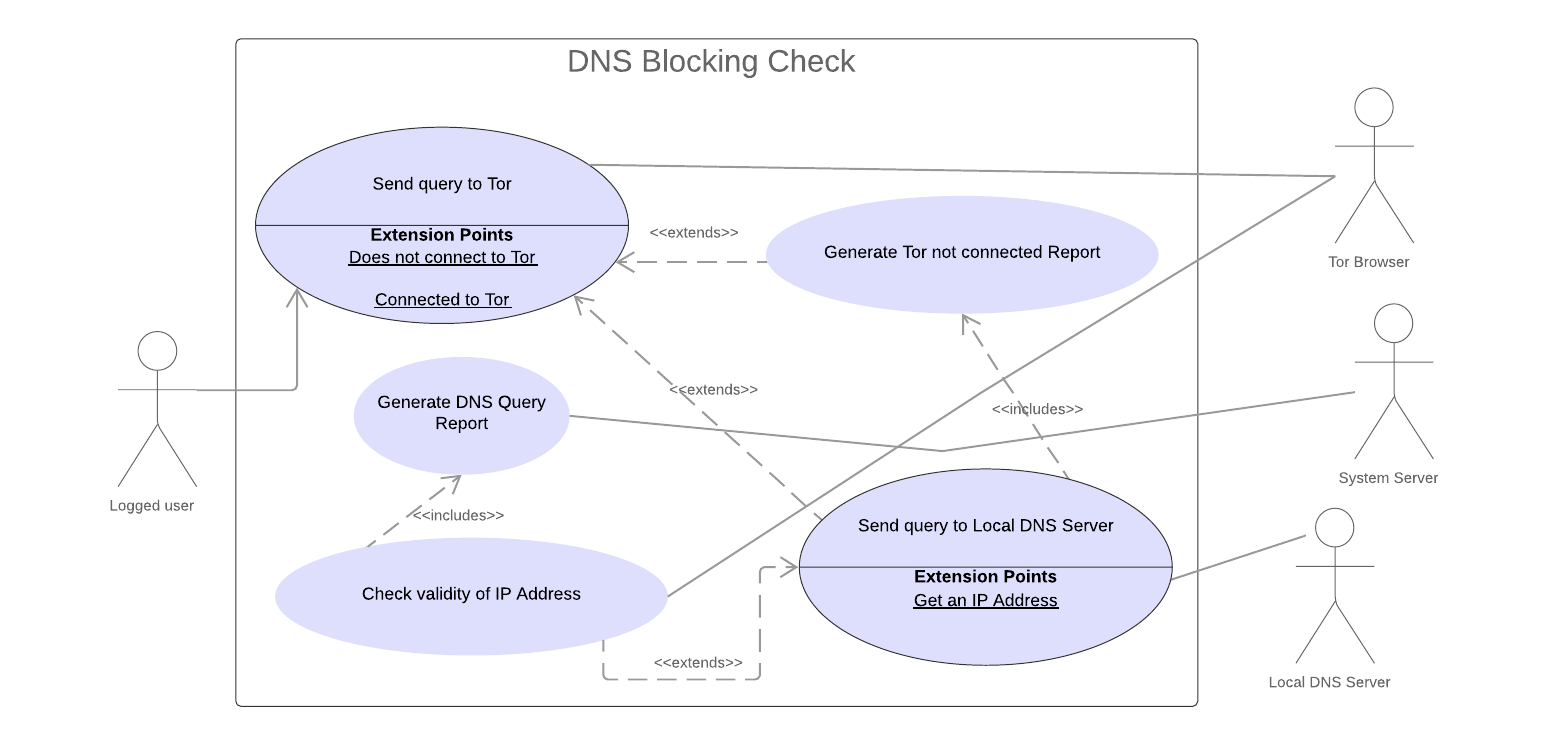
\includegraphics[width=\textwidth]{Diagrams/ucdns.png}
    \caption{Use-Case: Dns Censorship Analysis}
    \label{fig:ucdns}
\end{figure}

\begin{figure}[H]
    \centering
    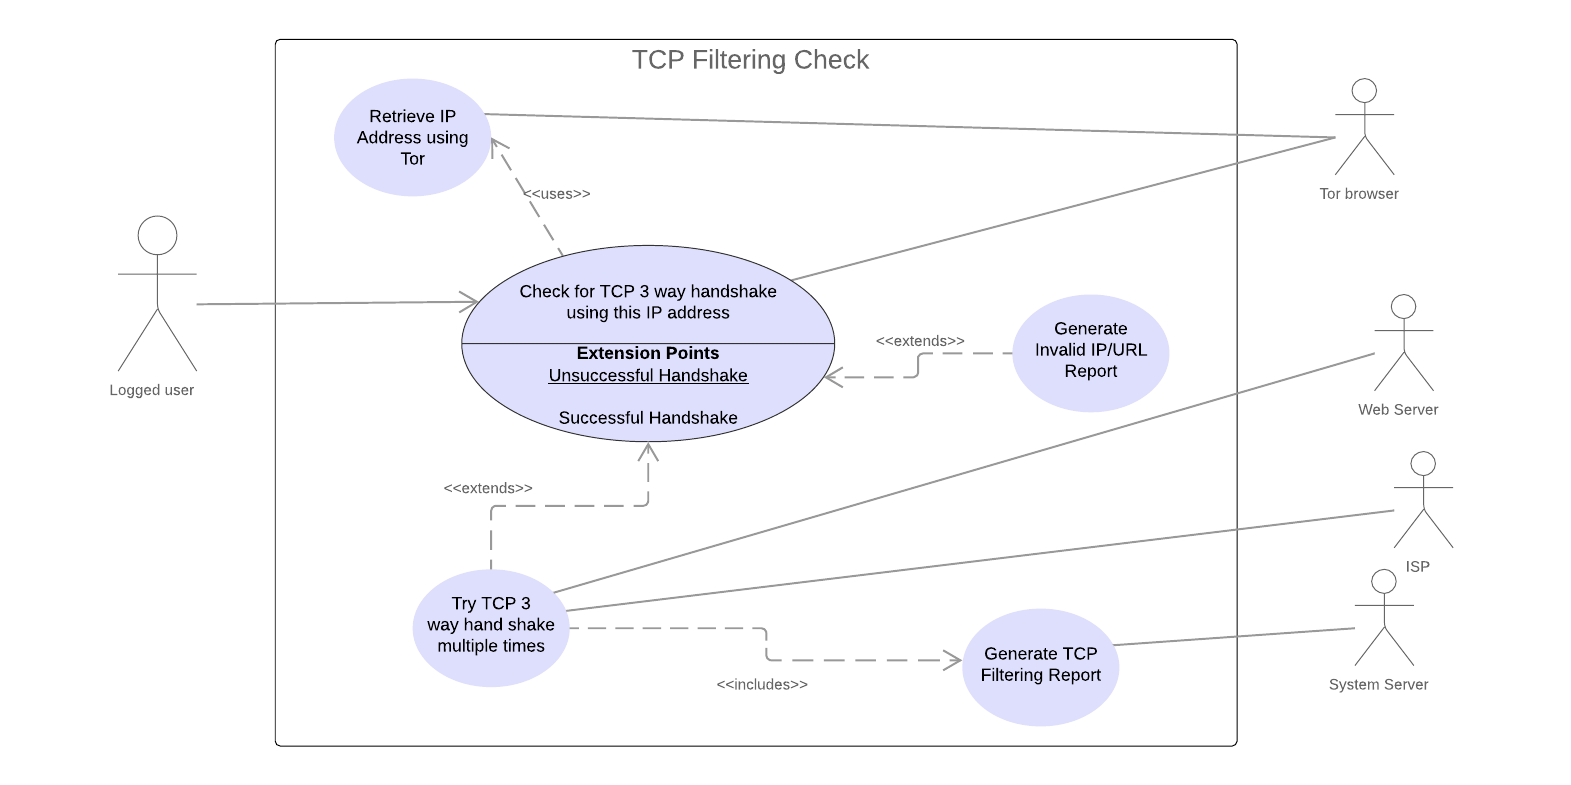
\includegraphics[width=\textwidth]{Diagrams/uctcp.png}
    \caption{Use-Case: TCP Censorship Analysis}
    \label{fig:ucdns}
\end{figure}

\begin{figure}[H]
    \centering
    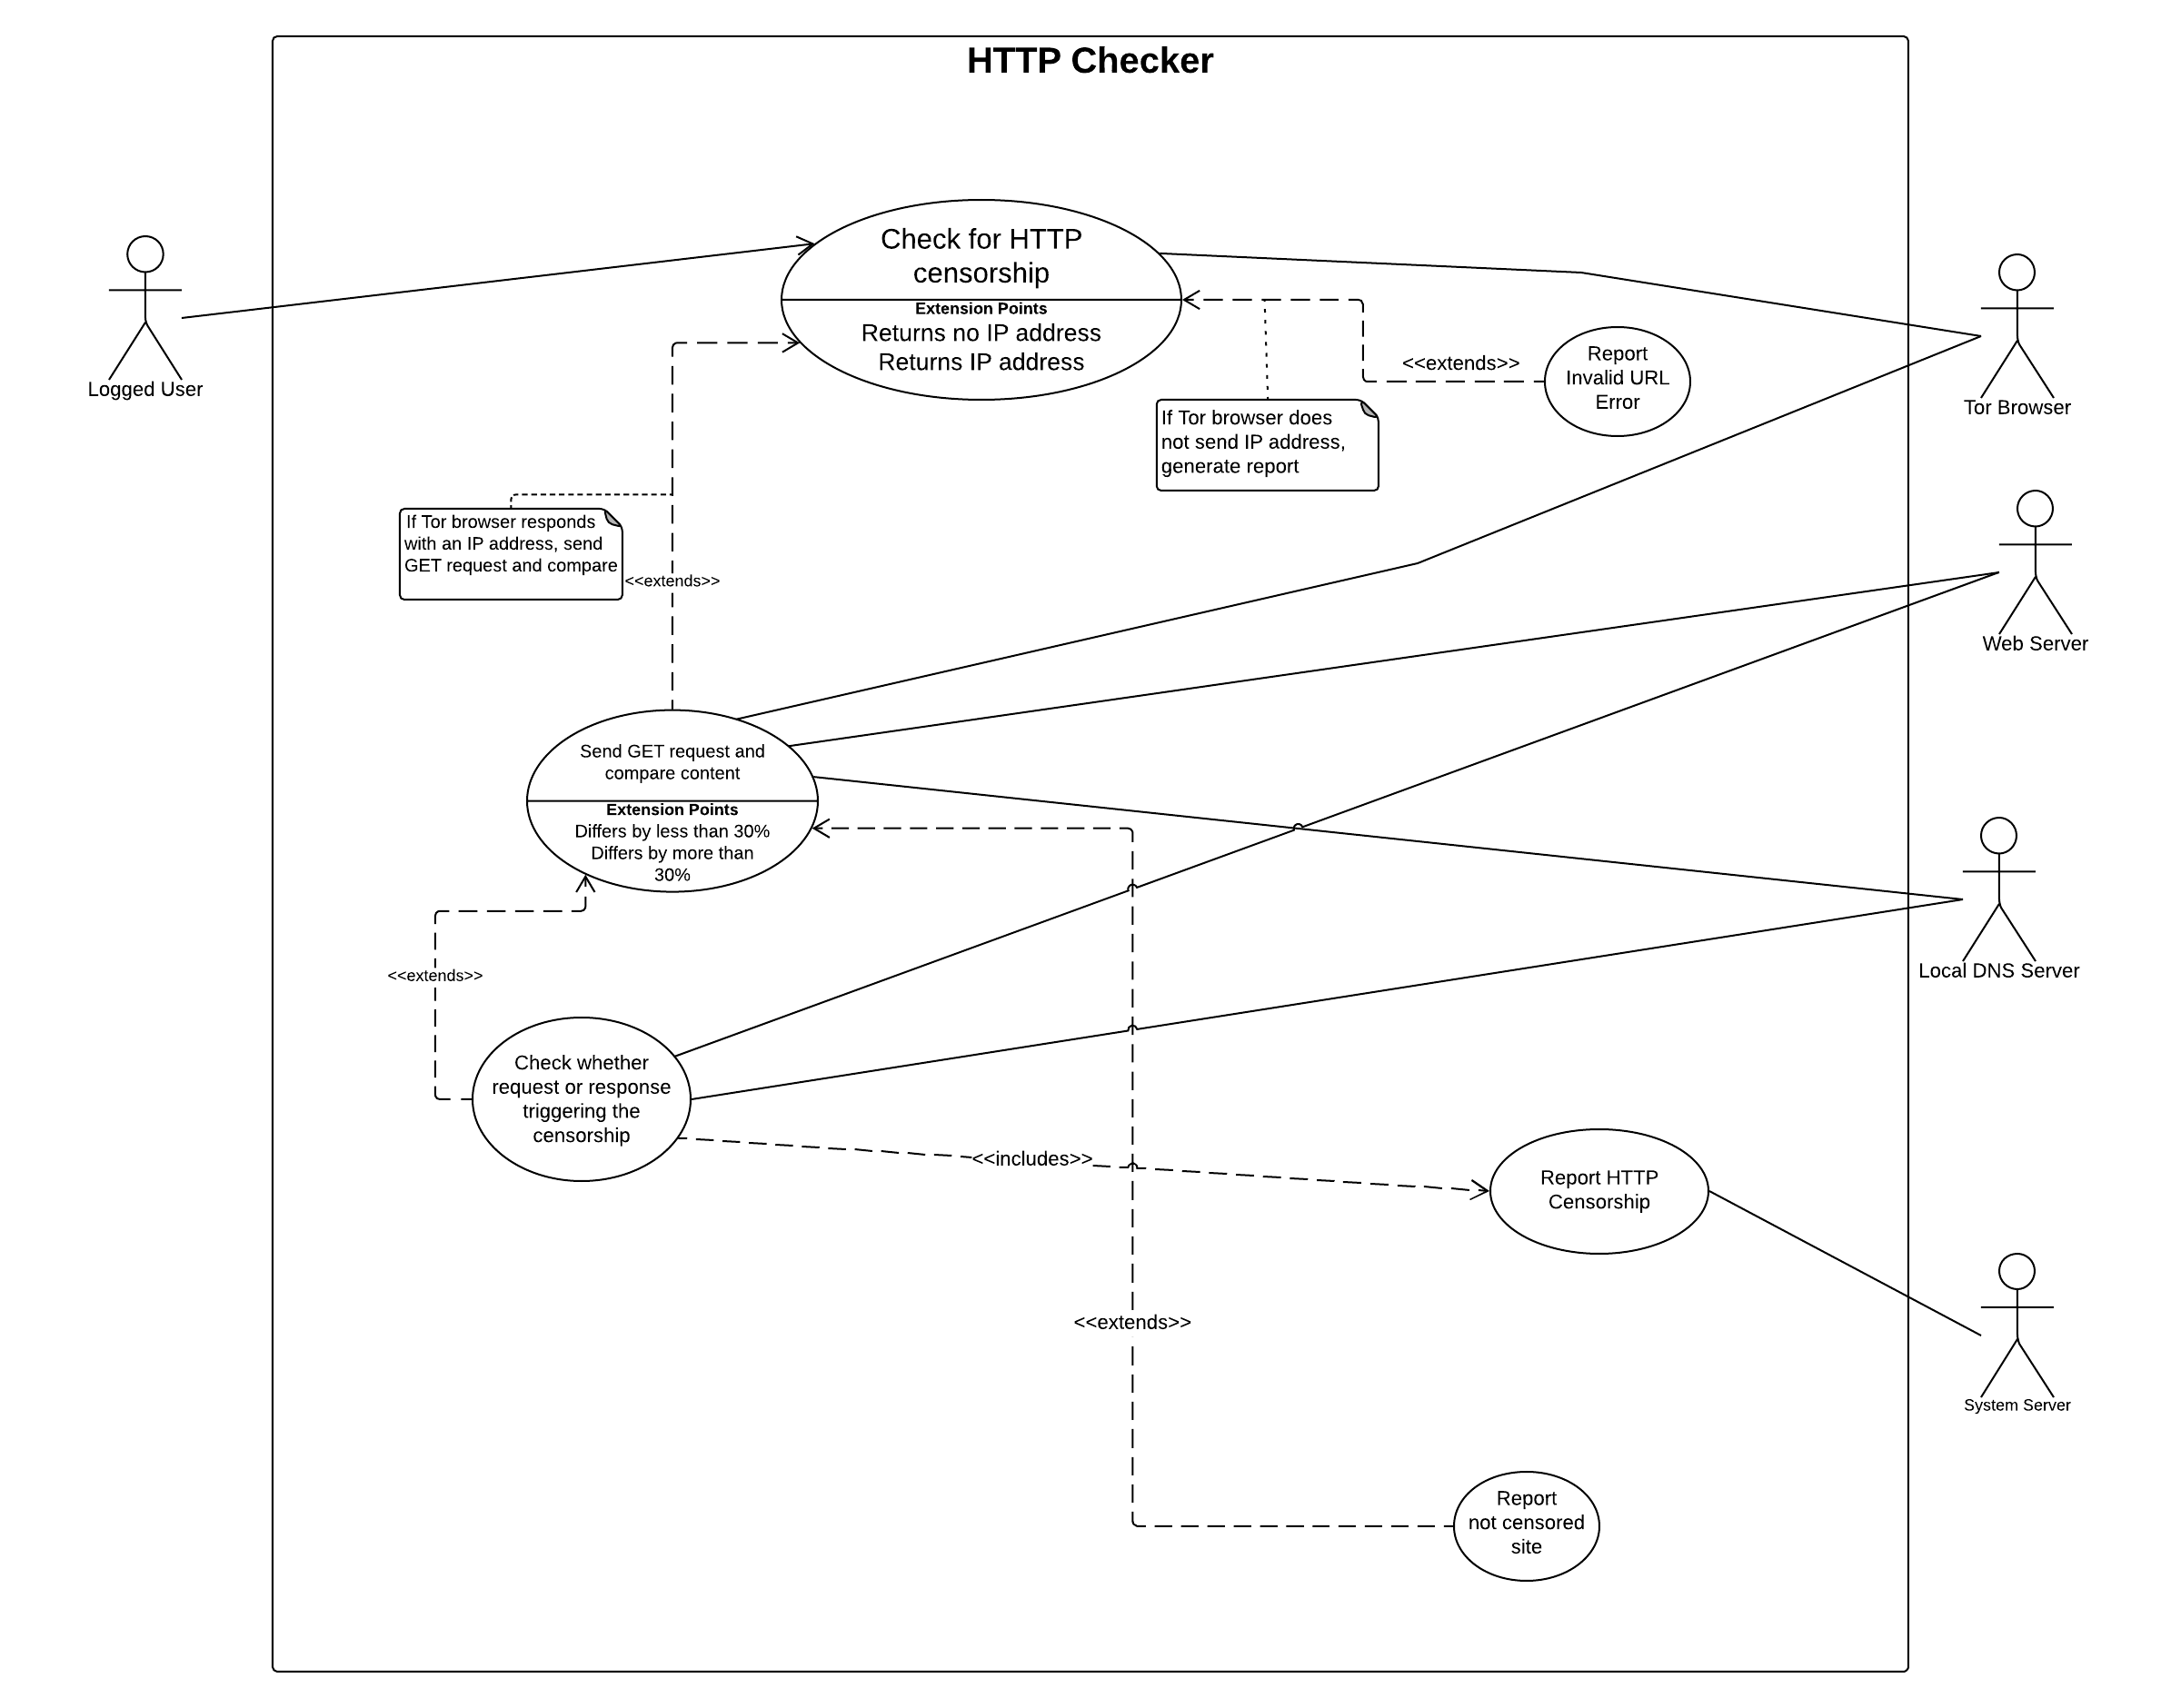
\includegraphics[width=\textwidth]{Diagrams/uchttp.png}
    \caption{Use-Case: HTTP Censorship Analysis}
    \label{fig:ucdns}
\end{figure}

\subsection{Entity Relationship Diagram (ERD)}
\begin{figure}[H]
    \centering
    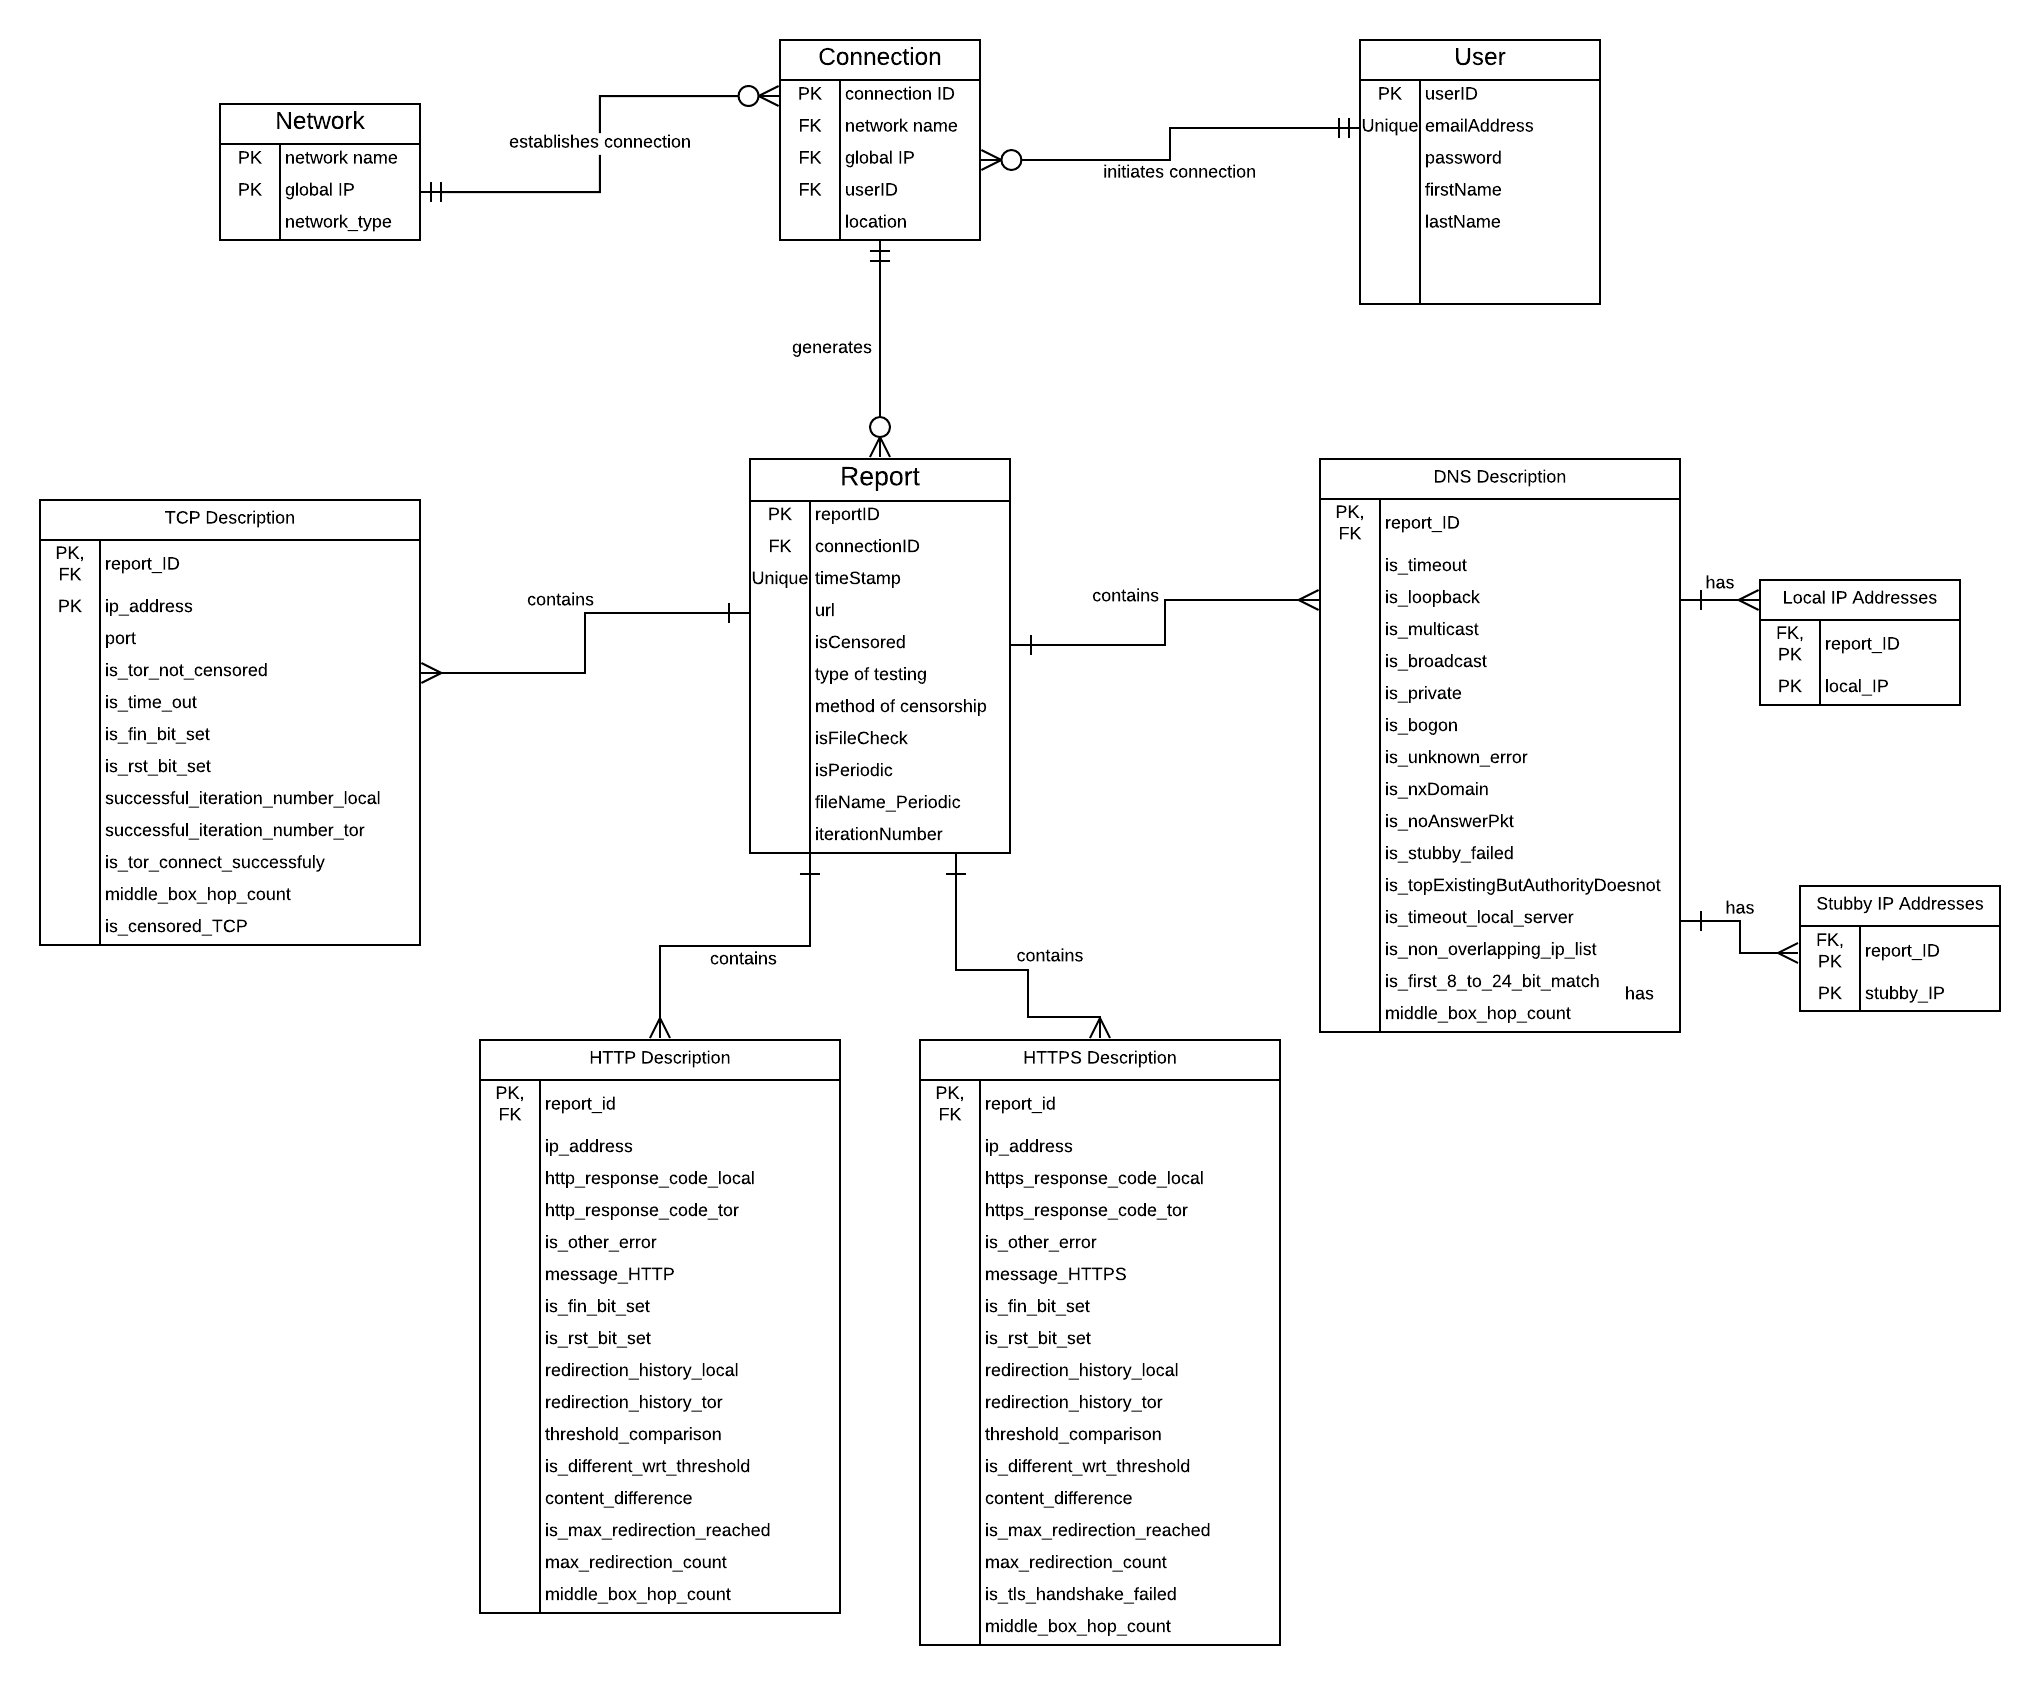
\includegraphics[width=\textwidth]{Diagrams/ERD_latest.png}
    \caption{Entity Relationship Diagram}
    \label{fig:ucdns}
\end{figure}

\subsection{Class Diagrams}

\begin{figure}[H]
    \centering
    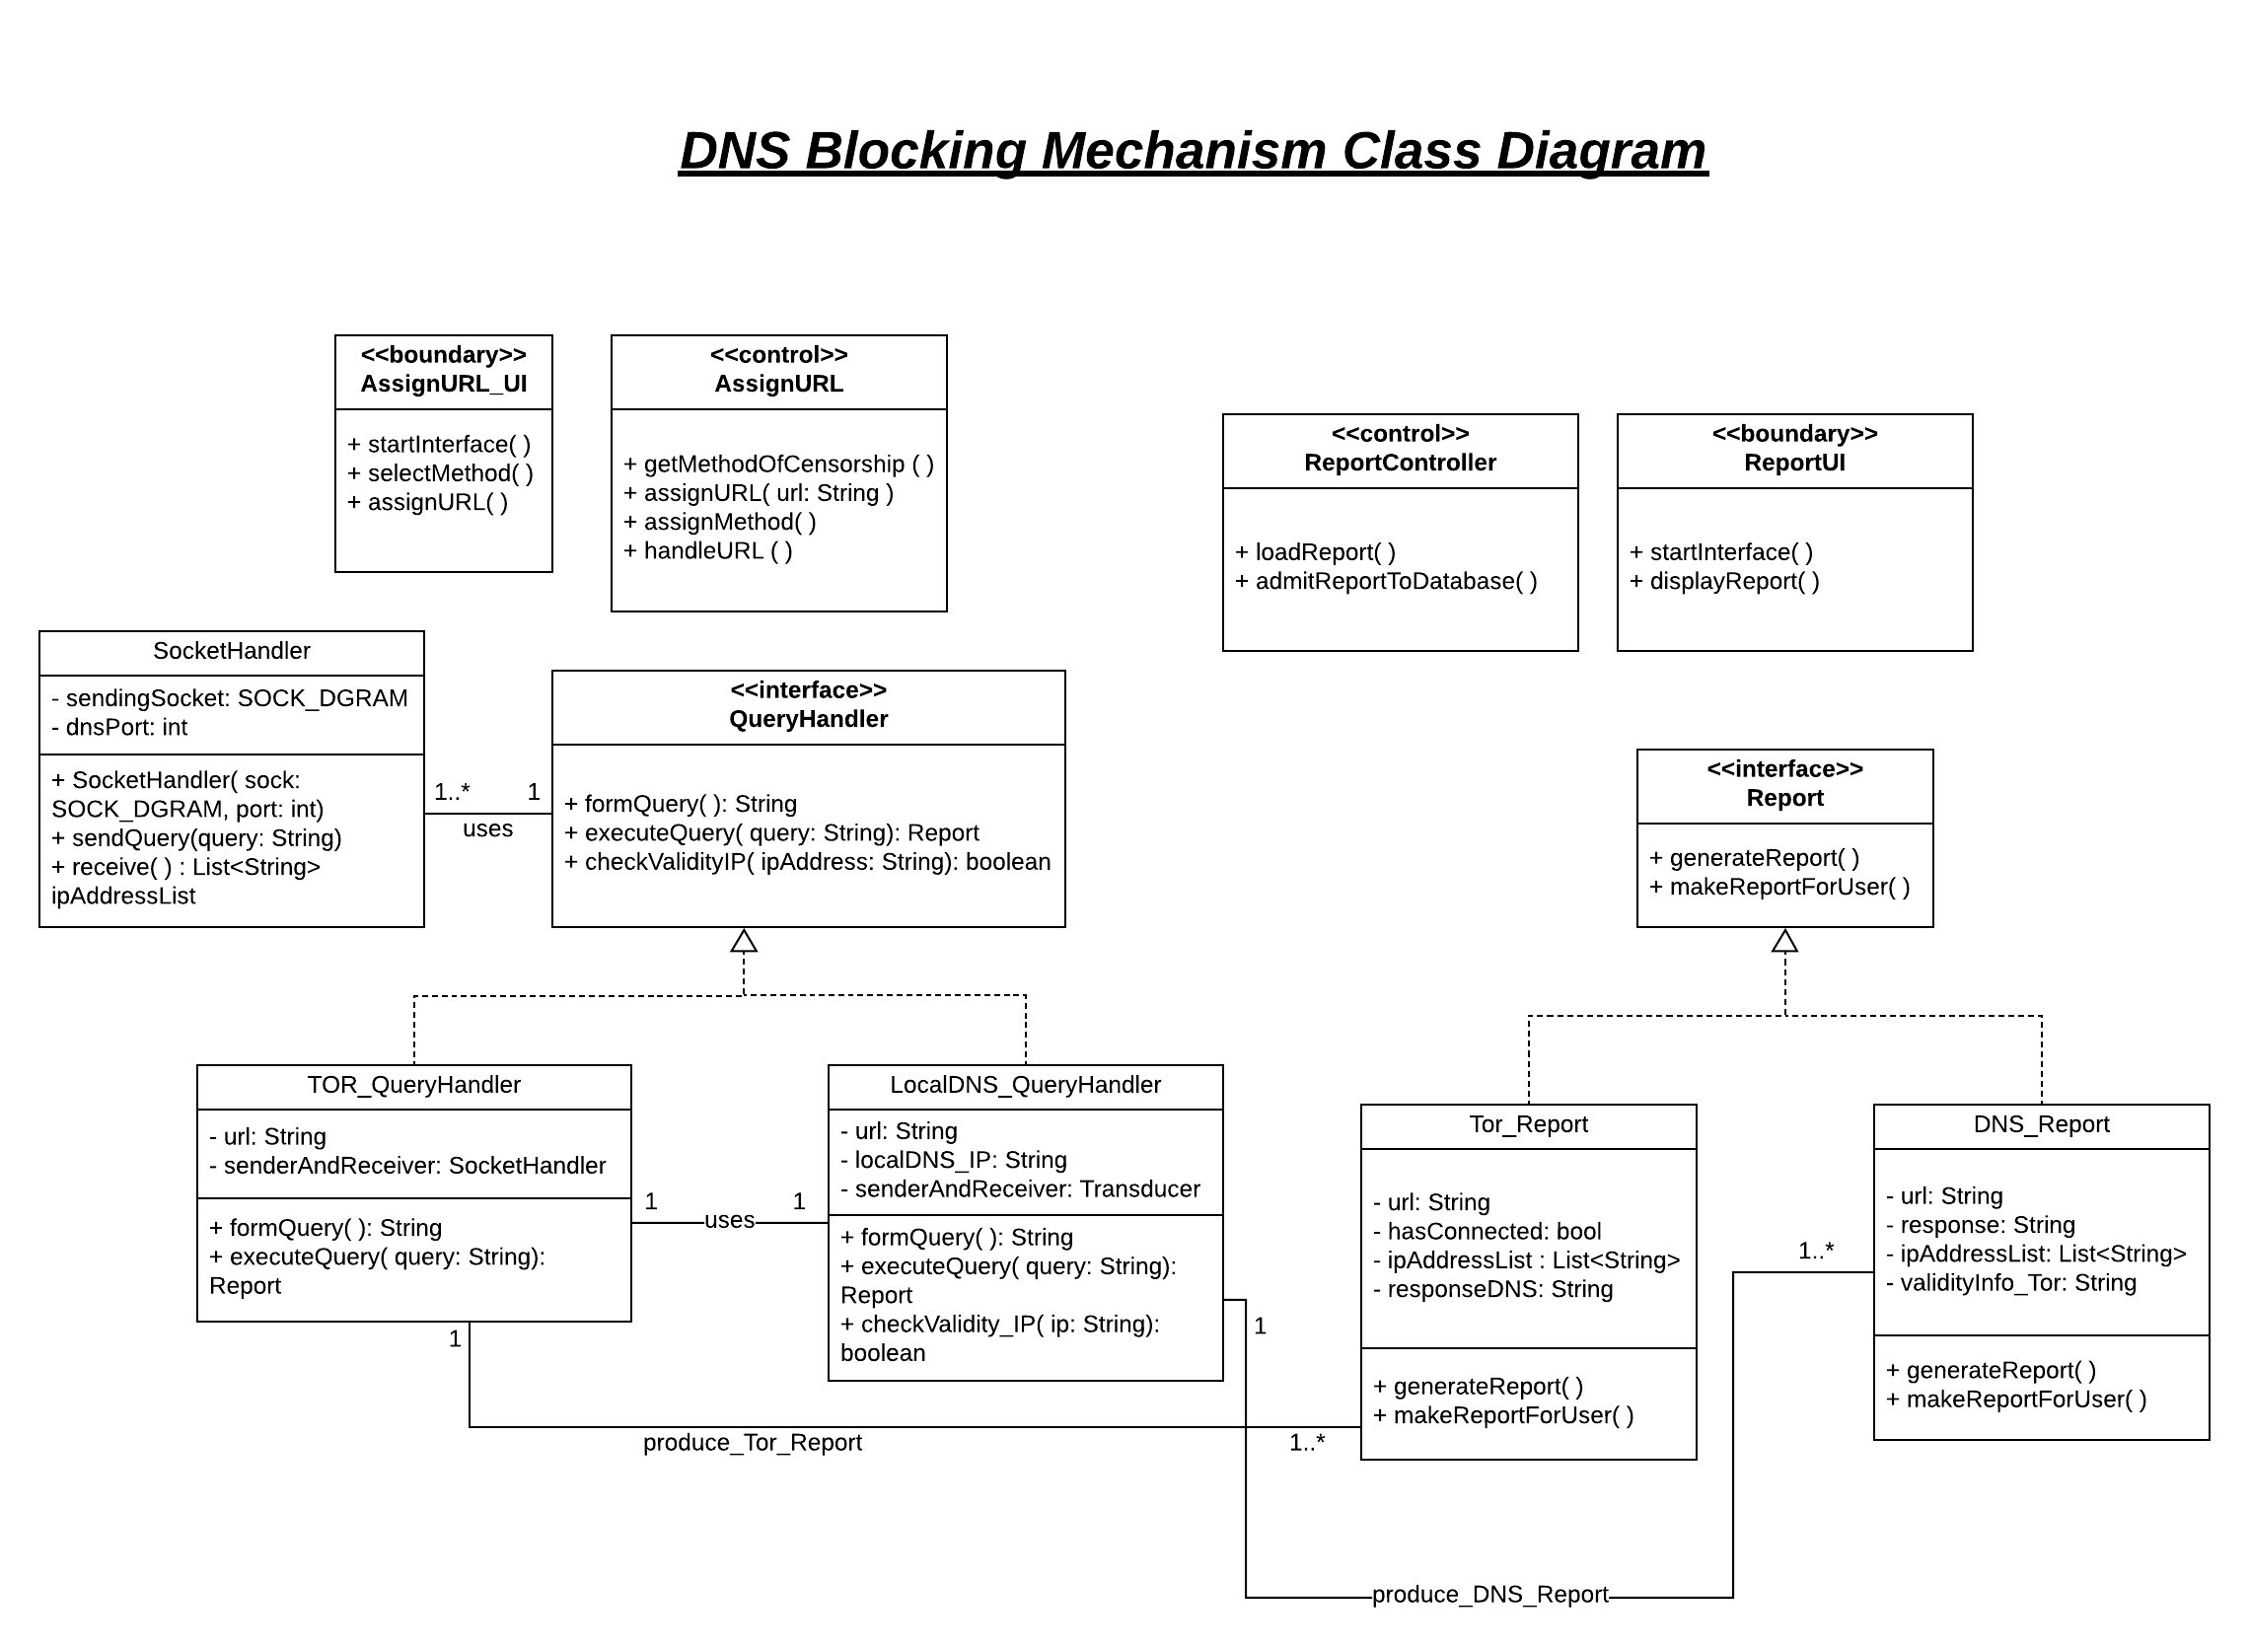
\includegraphics[width=\textwidth]{Diagrams/cddns.png}
    \caption{Class Diagram: Dns Censorship Analysis}
    \label{fig:ucdns}
\end{figure}

\begin{figure}[H]
    \centering
    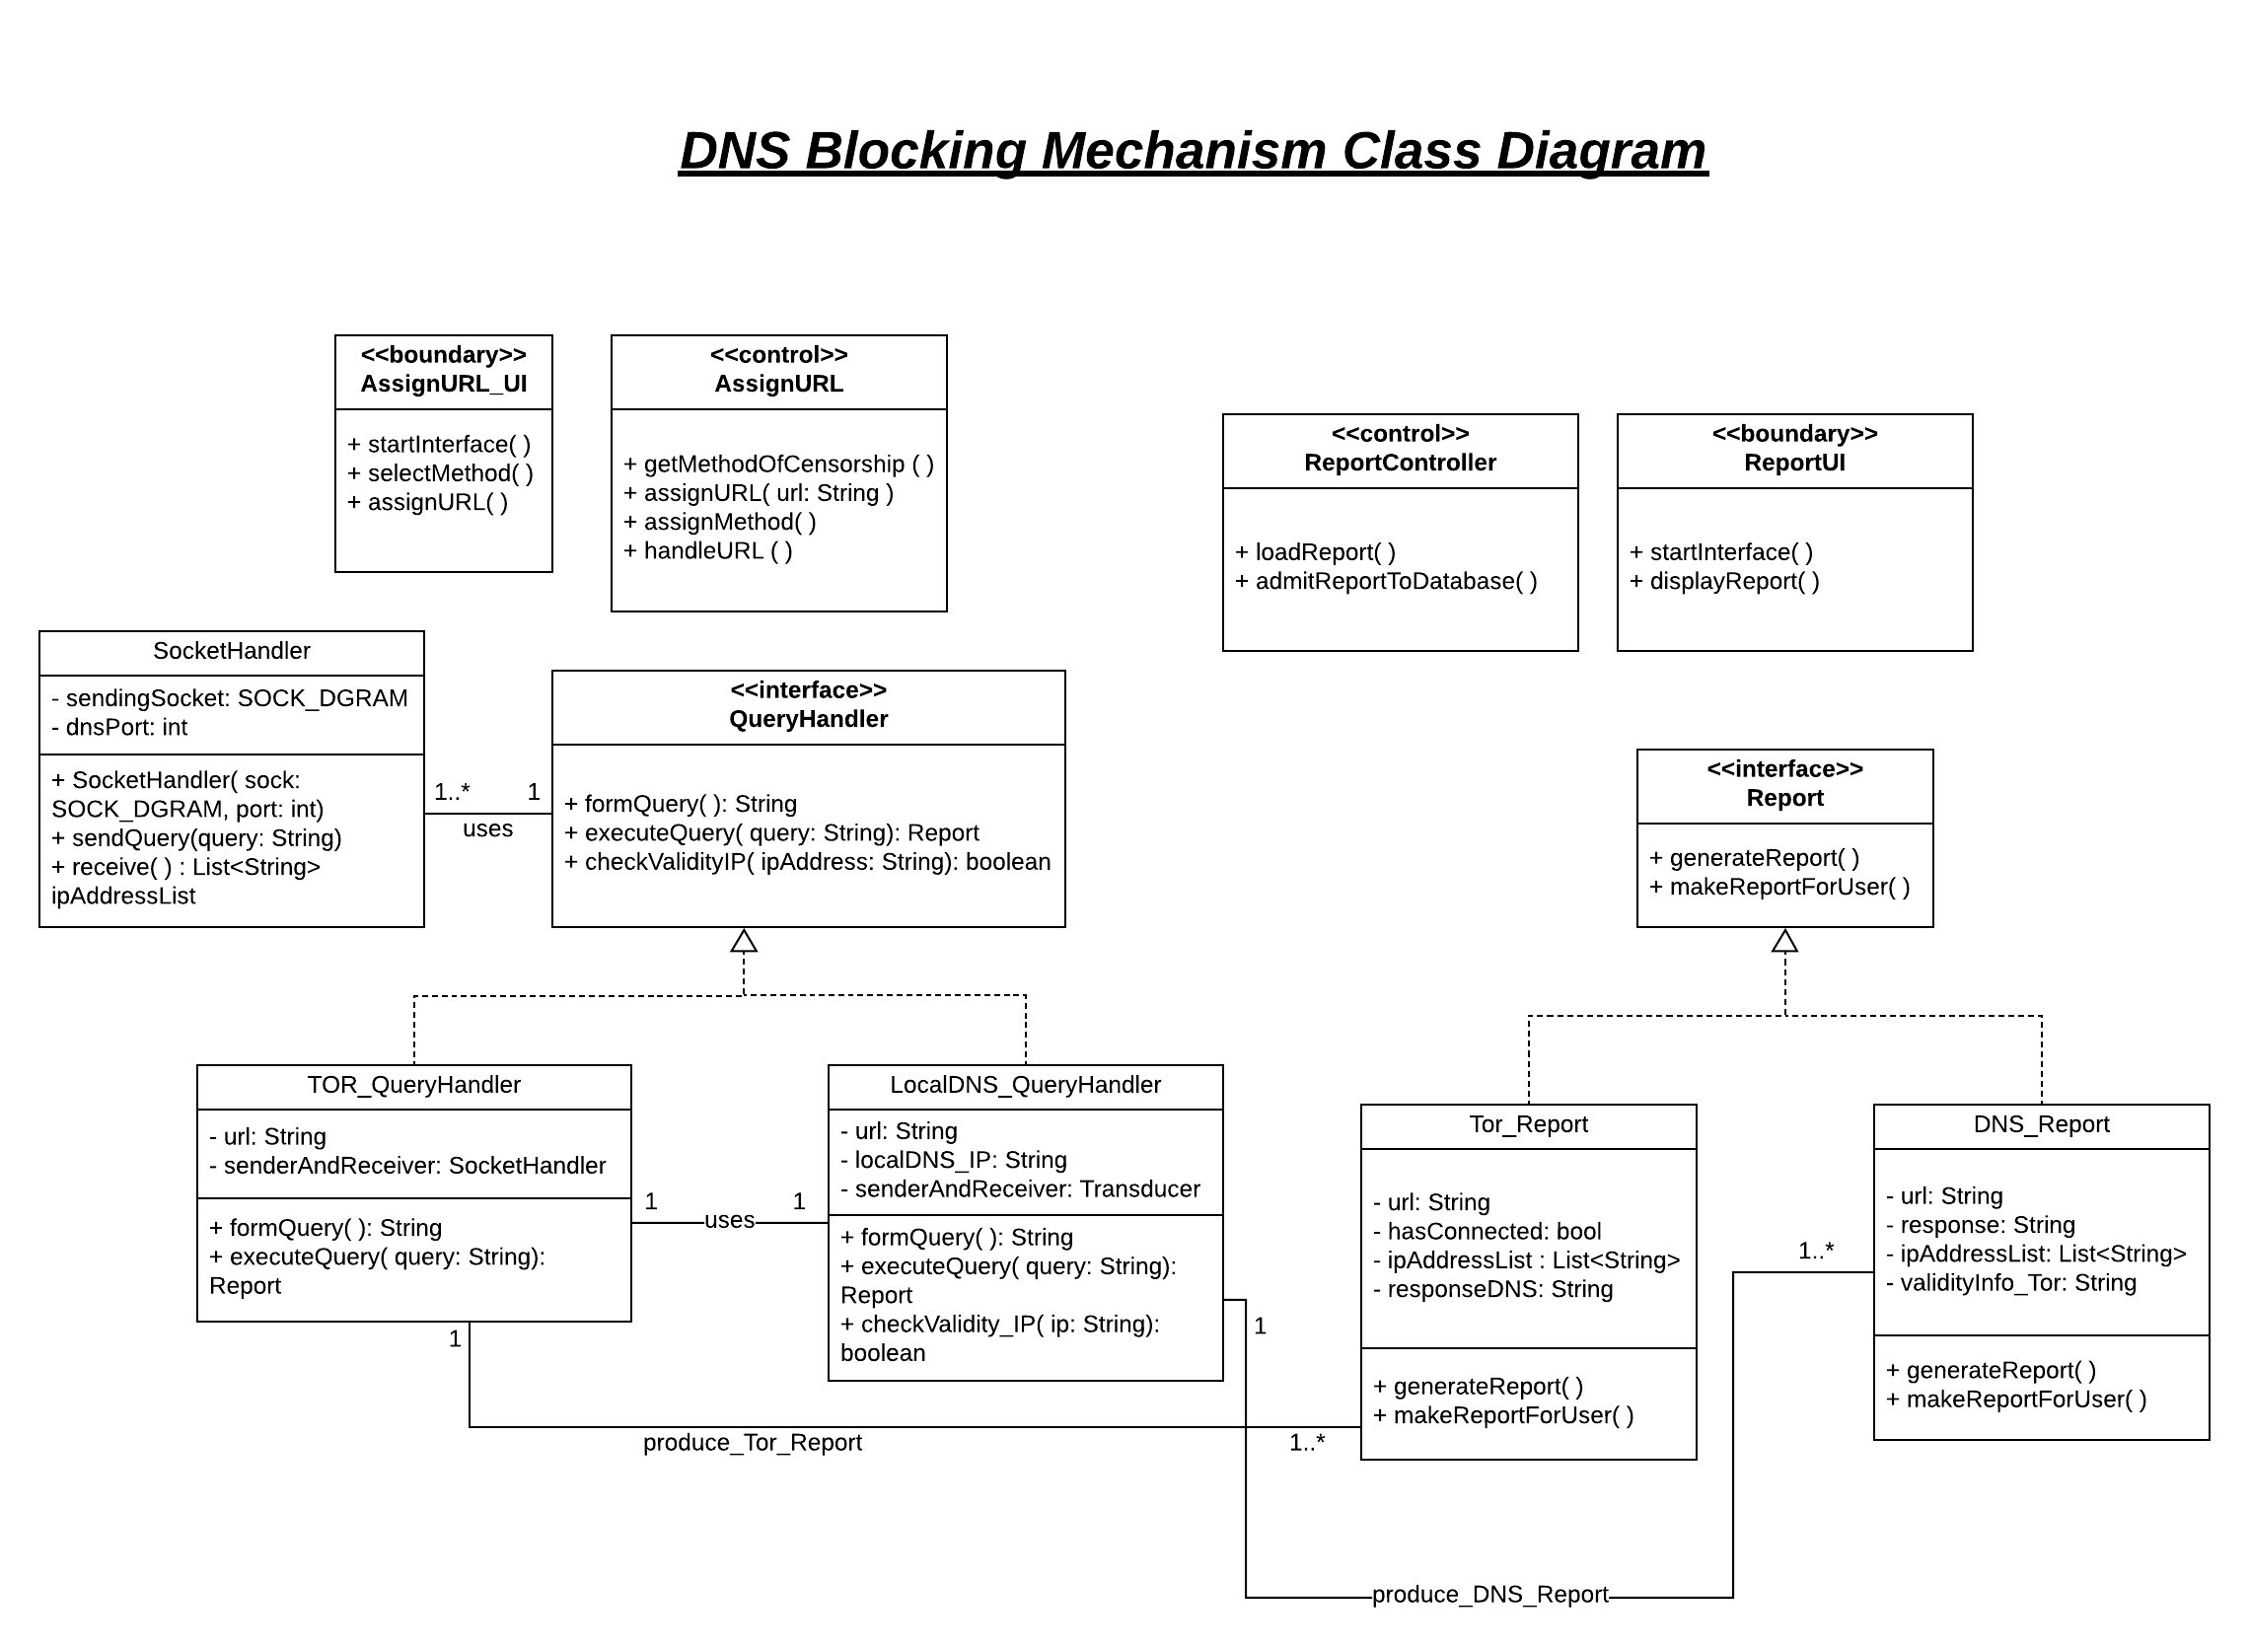
\includegraphics[width=\textwidth]{Diagrams/cddns.png}
    \caption{Class Diagram: TCP Censorship Analysis}
    \label{fig:ucdns}
\end{figure}

\begin{figure}[H]
    \centering
    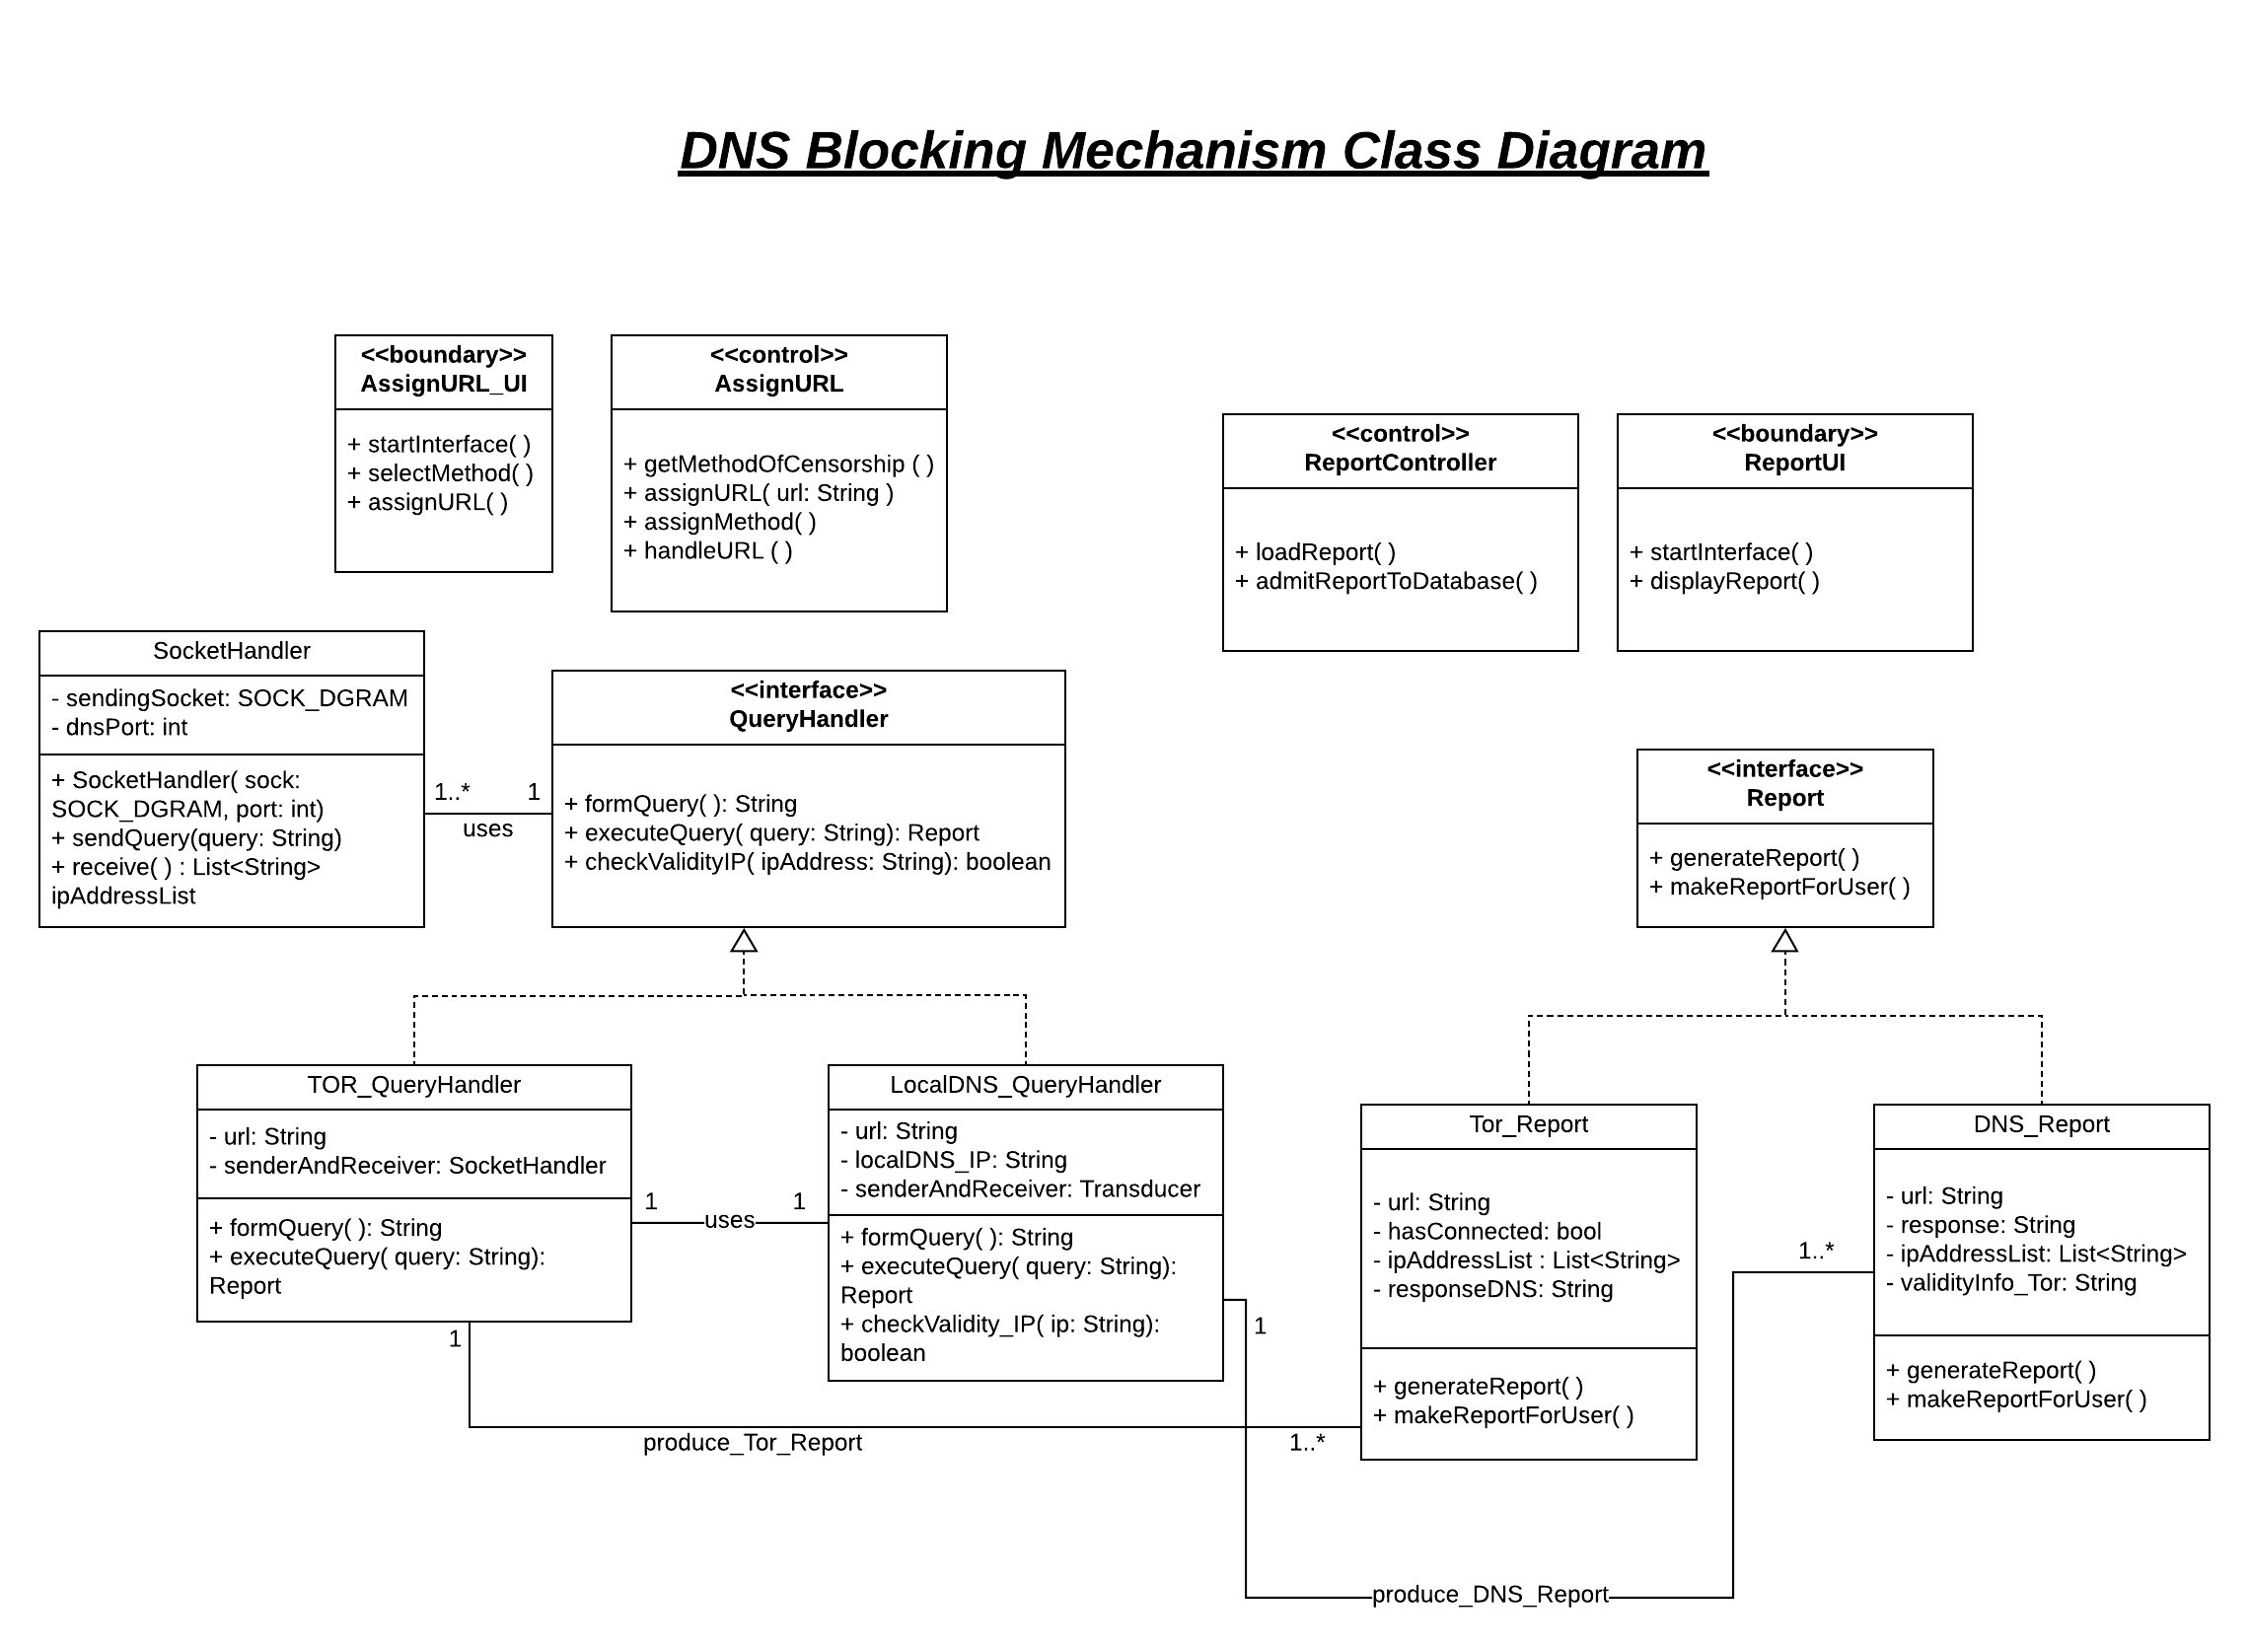
\includegraphics[width=\textwidth]{Diagrams/cddns.png}
    \caption{Class Diagram: HTTP Censorship Analysis}
    \label{fig:ucdns}
\end{figure}


\section{User Guide}
\subsection{First step: Registration through website}
First of all, a user must register through website. Here he/she should give username, valid email and password for registration. 
\begin{figure}[h]
    \centering
    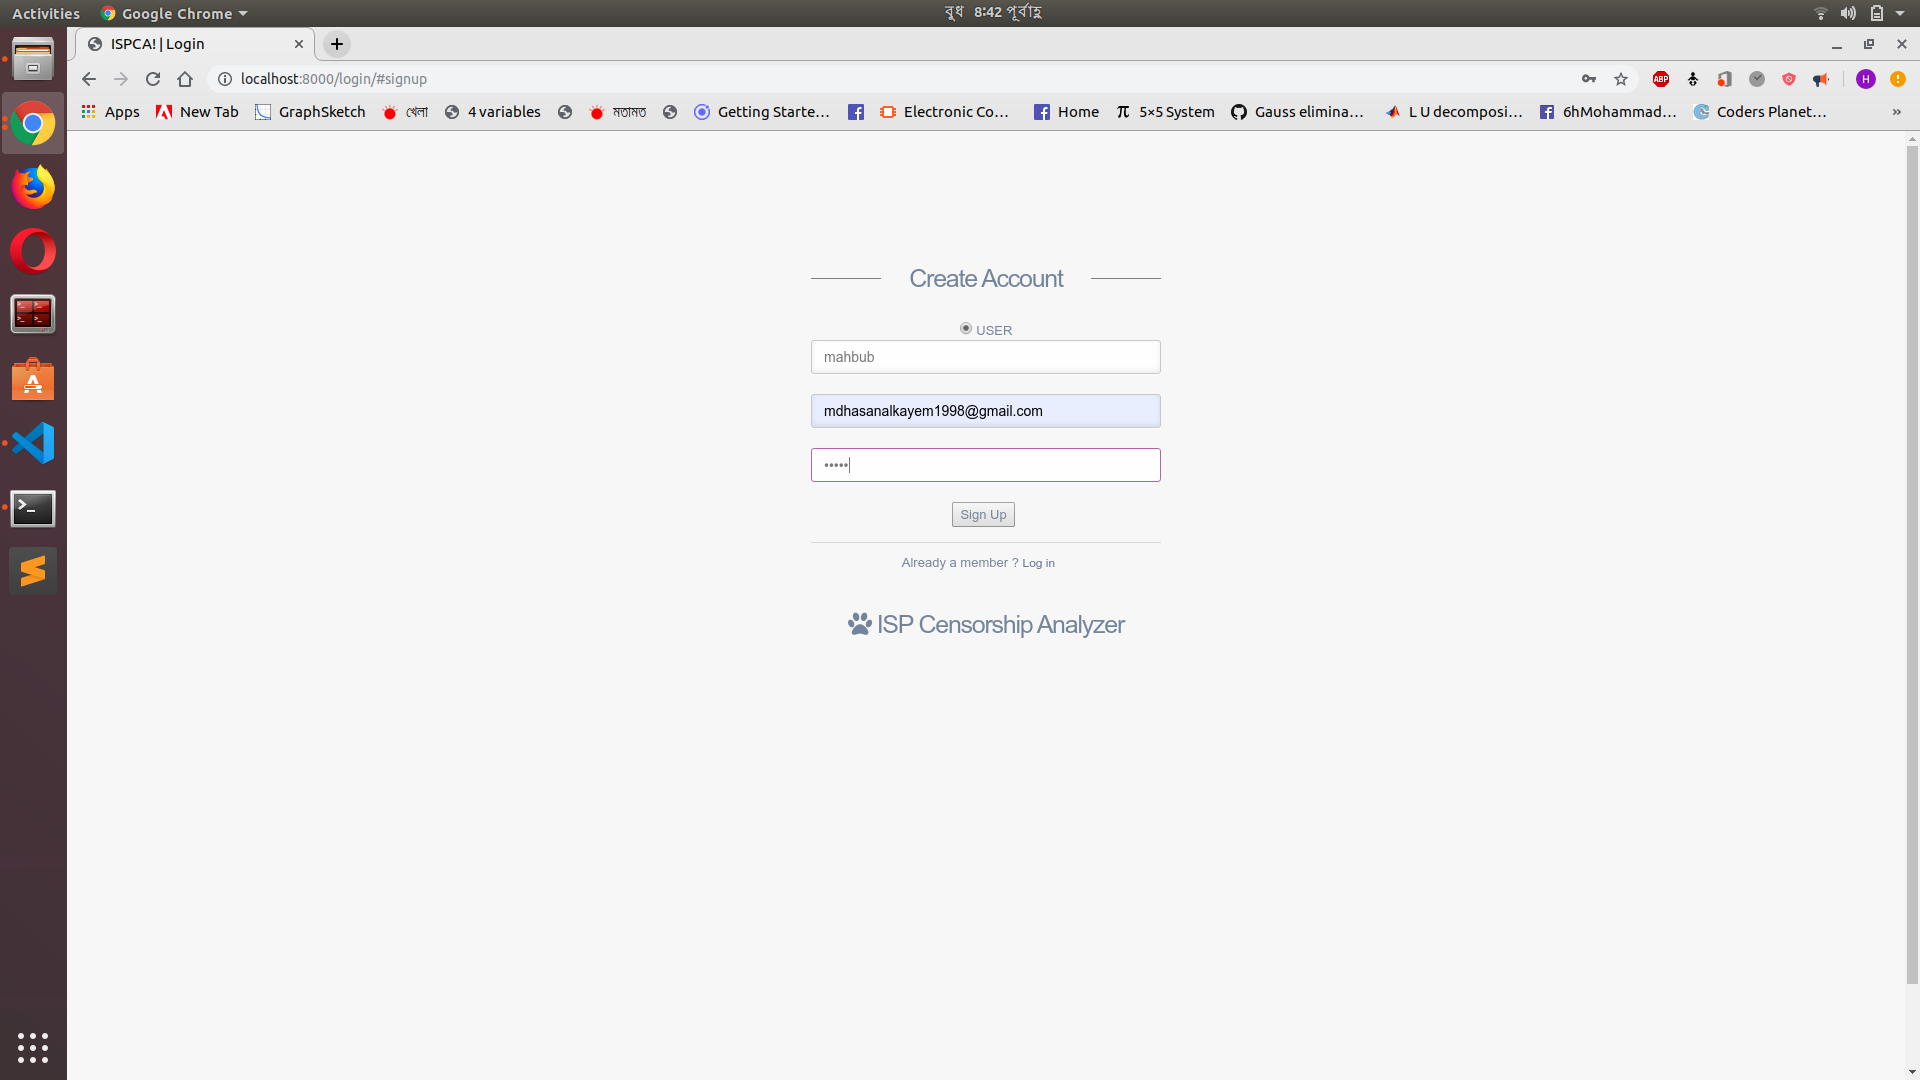
\includegraphics[width=\textwidth]{website/13registration.png}
    \caption{Insert Compulsory field for registration}
    \label{fig:web1}
\end{figure}
If registration becomes successful, a login window will be shown and he can use the desktop app.
\begin{figure}[h]
    \centering
    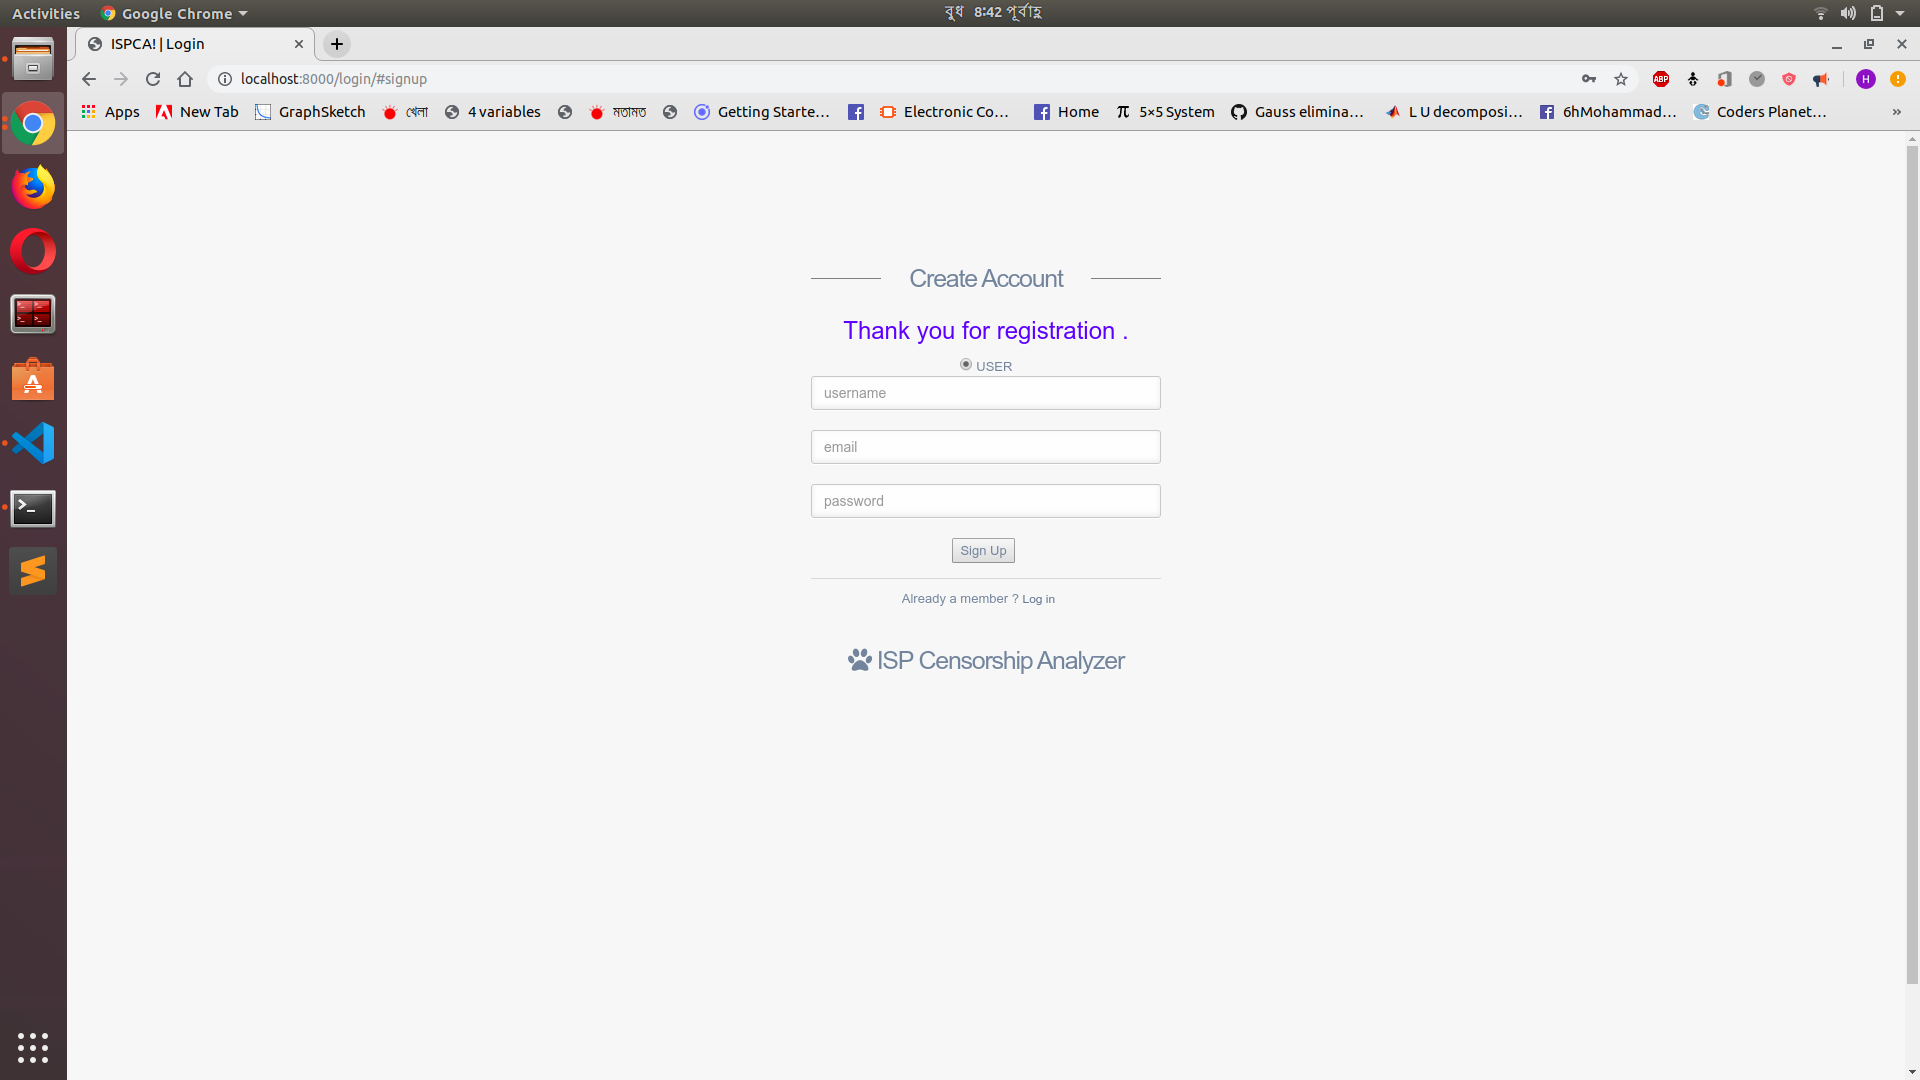
\includegraphics[width=\textwidth]{website/14registratin2.png}
    \caption{Valid registration}
    \label{fig:web2}
\end{figure}


\subsection{Second step: Login through desktop app}
\input{kayemtex/secondstep.tex}


\subsection{Third step: Checking censorship}
Here all the procedure of the system are given in caption of the pictures.
A user will come into his home page after successful login. All information regarding Network ISP are given in home page and 
\begin{figure}[h]
    \centering
    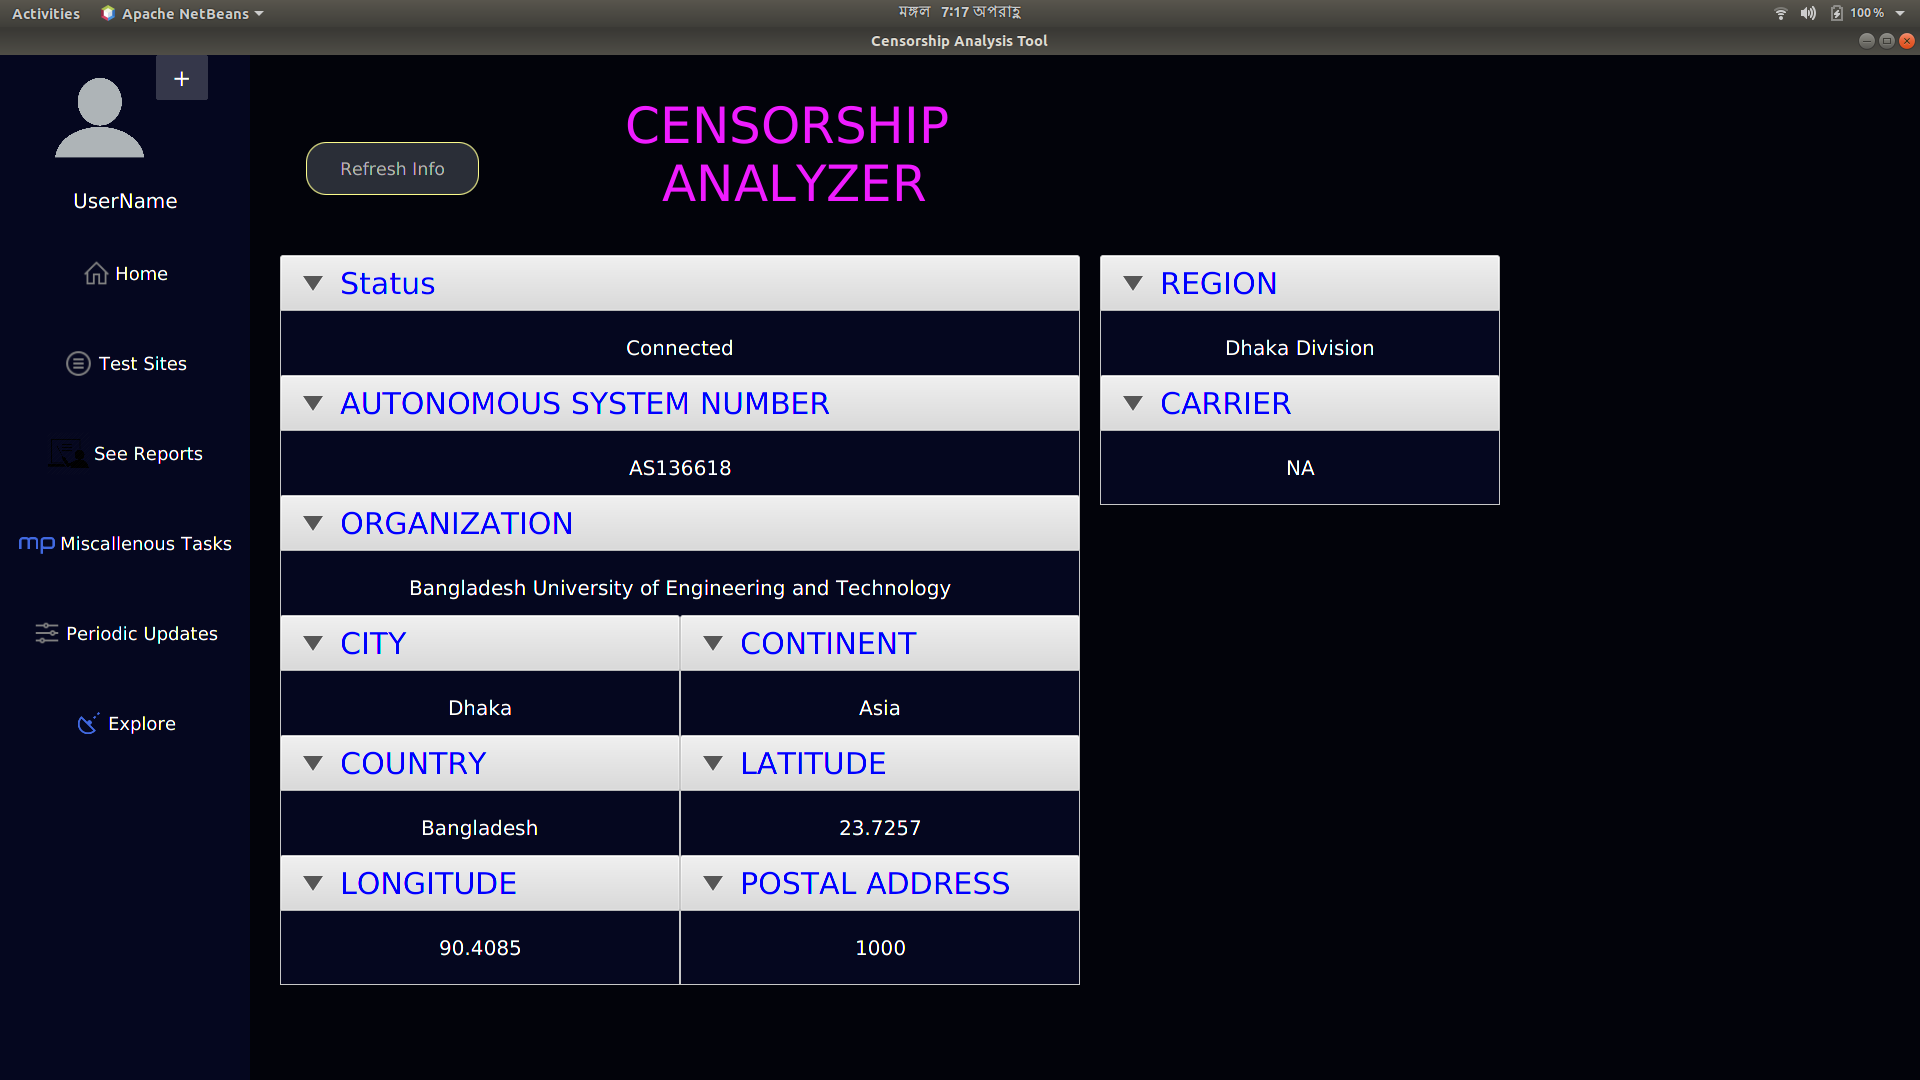
\includegraphics[width=\textwidth]{usersite/home.png}
    \caption{Home page at desktop app}
    \label{fig:user0}
\end{figure}

A user can see his previous reports by clicking \emph{See Reports} button of home page.
He will see all the reports . He can apply various filter on it and after clicking \emph{Refresh} button, he will see filtered test.

\begin{figure}[h]
    \centering
    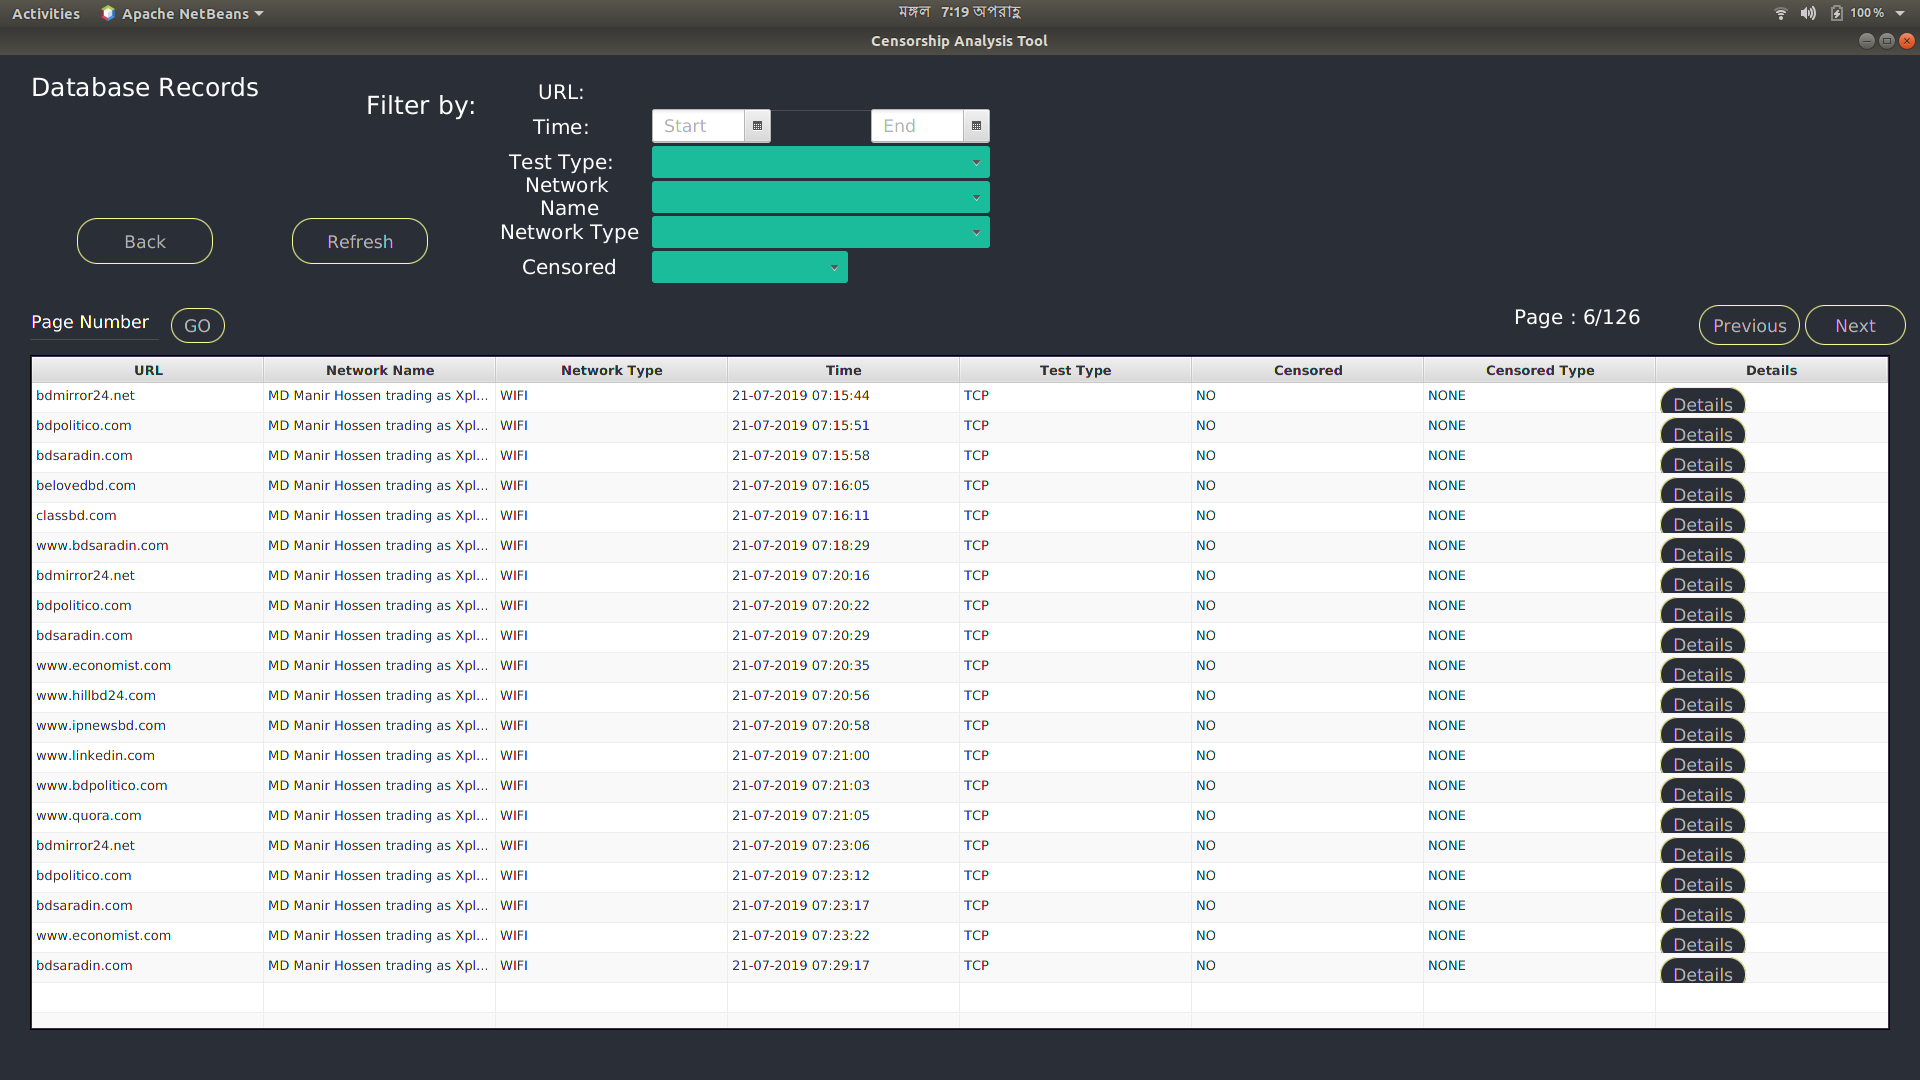
\includegraphics[width=\textwidth]{usersite/1recordswithoutfilter.png}
    \caption{Records without filtering}
    \label{fig:user1}
\end{figure}

\begin{figure}[h]
    \centering
    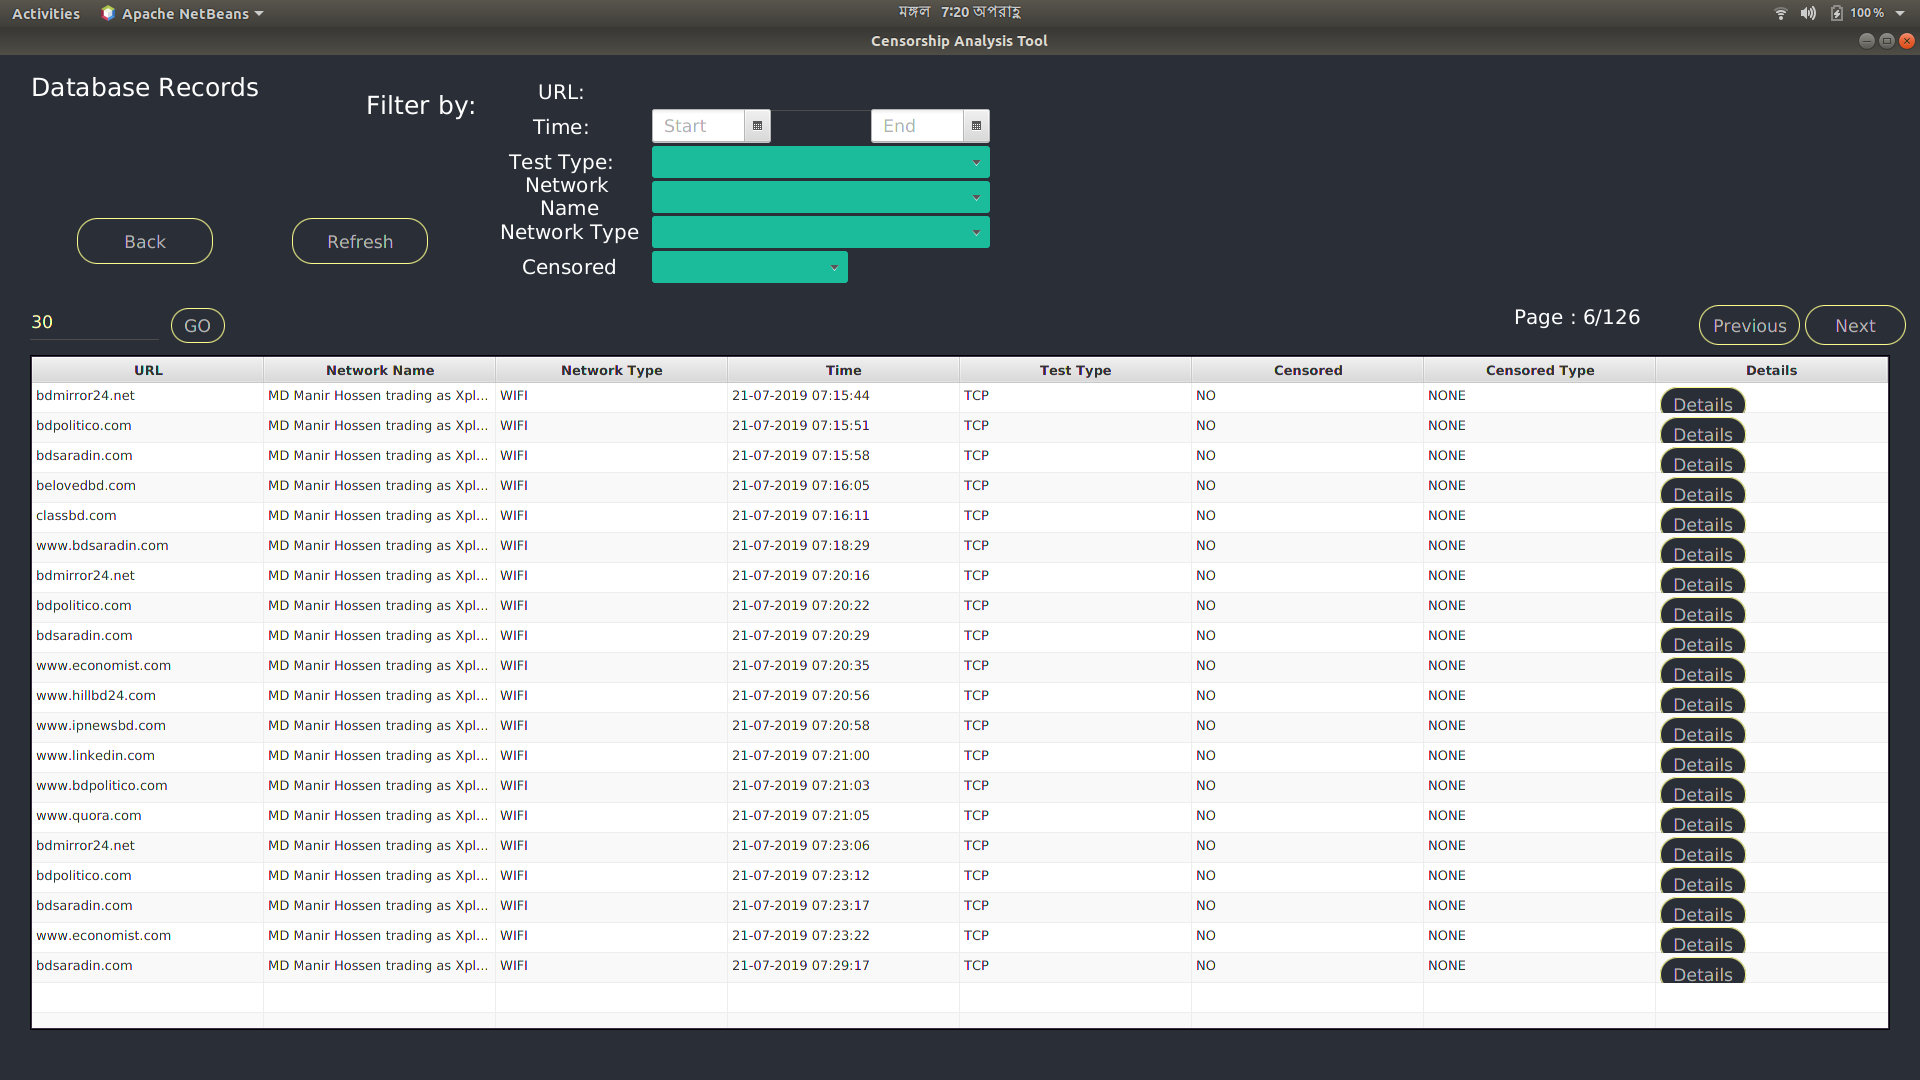
\includegraphics[width=\textwidth]{usersite/2pageinput.png}
    \caption{Inserting page 30}
    \label{fig:user2}
\end{figure}

\begin{figure}[h]
    \centering
    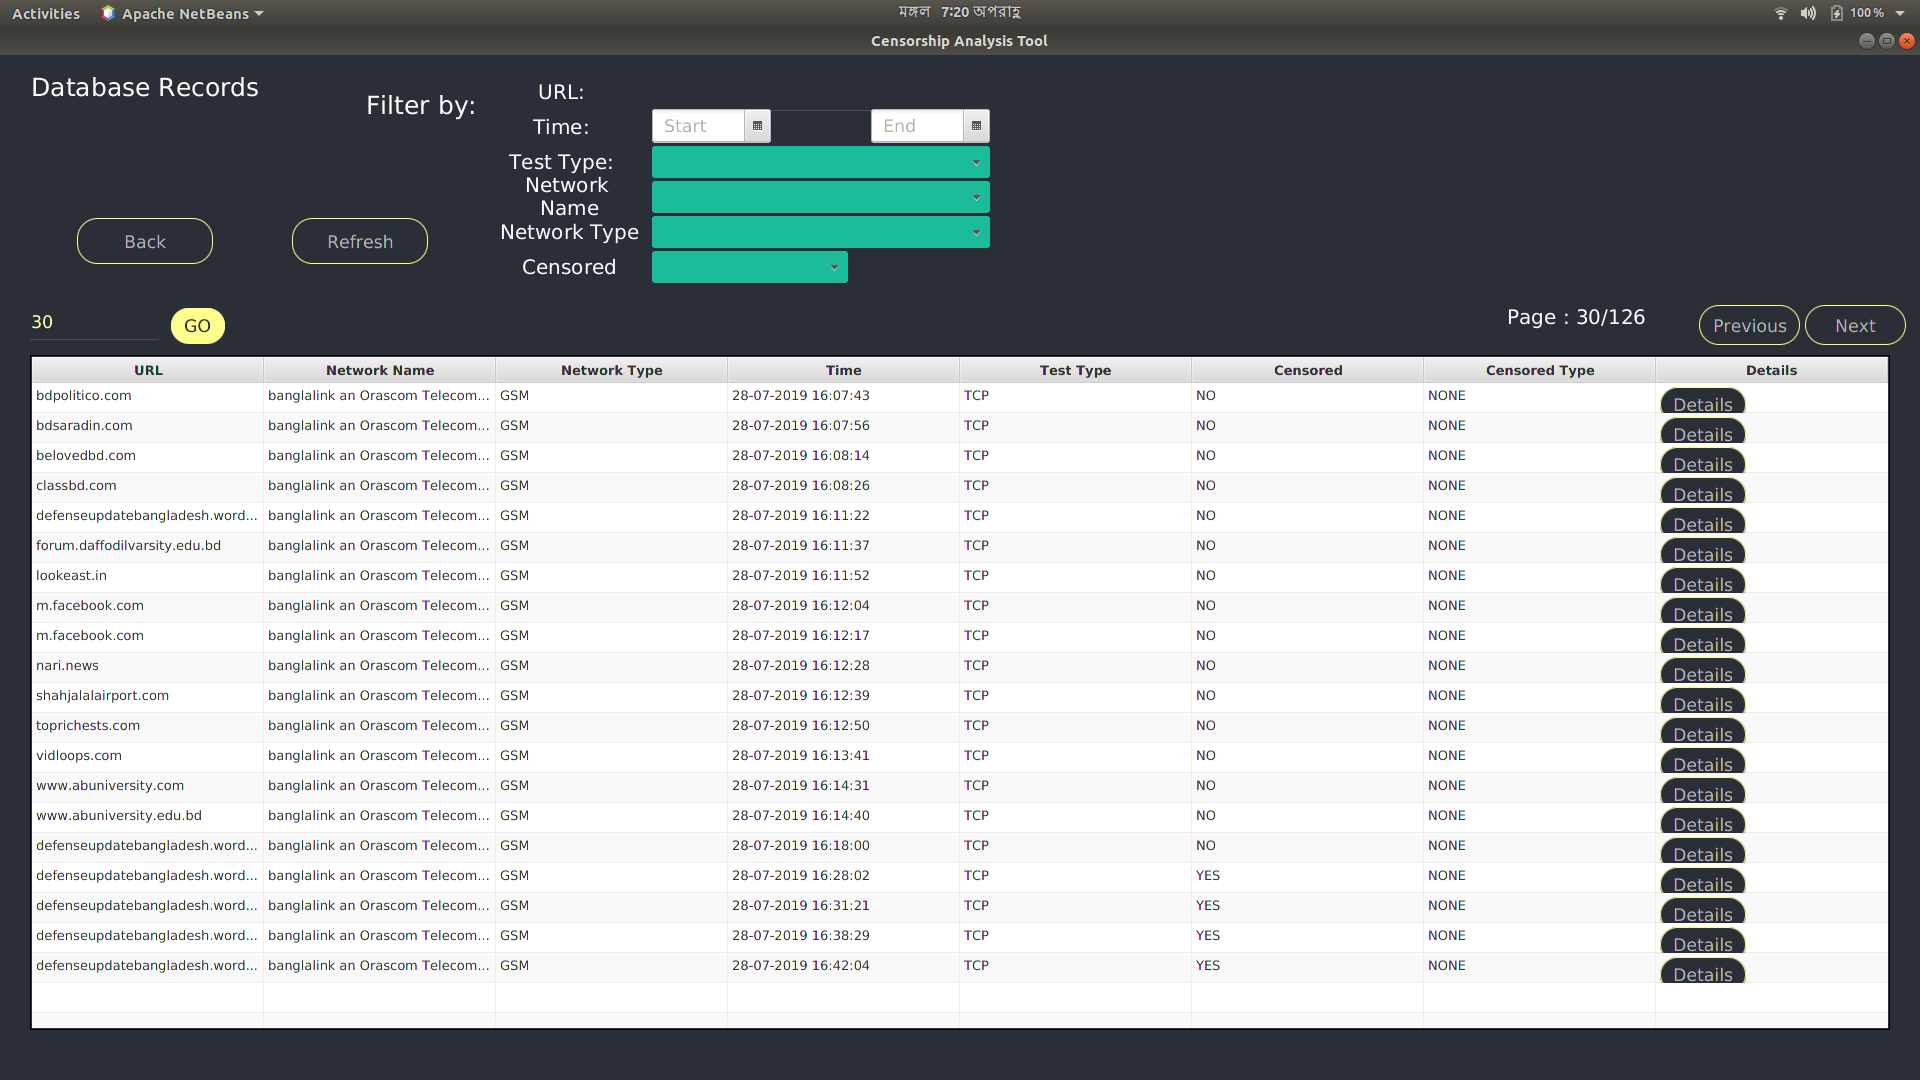
\includegraphics[width=\textwidth]{usersite/3pageoutput.png}
    \caption{At page 30}
    \label{fig:user3}
\end{figure}

\begin{figure}[h]
    \centering
    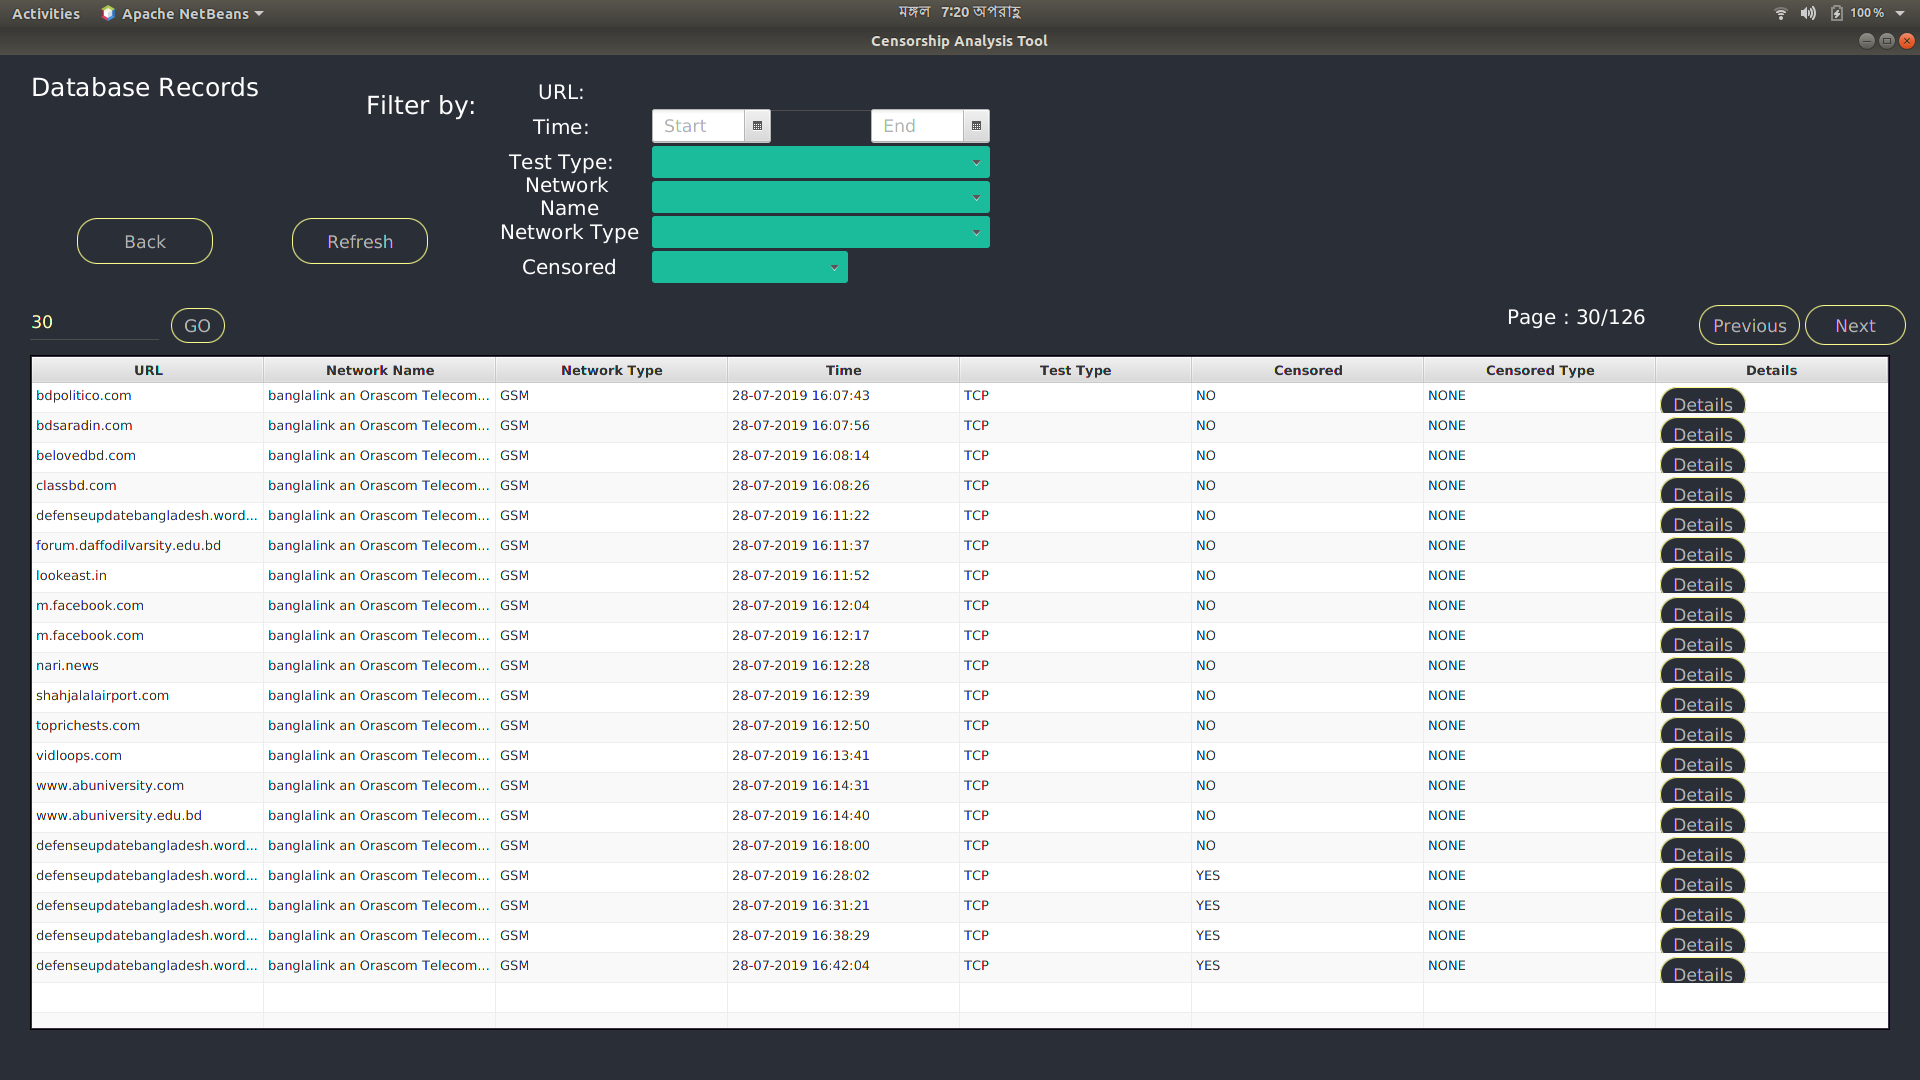
\includegraphics[width=\textwidth]{usersite/4withoutfilter.png}
    \caption{Agin test are without filter}
    \label{fig:user4}
\end{figure}

\begin{figure}[h]
    \centering
    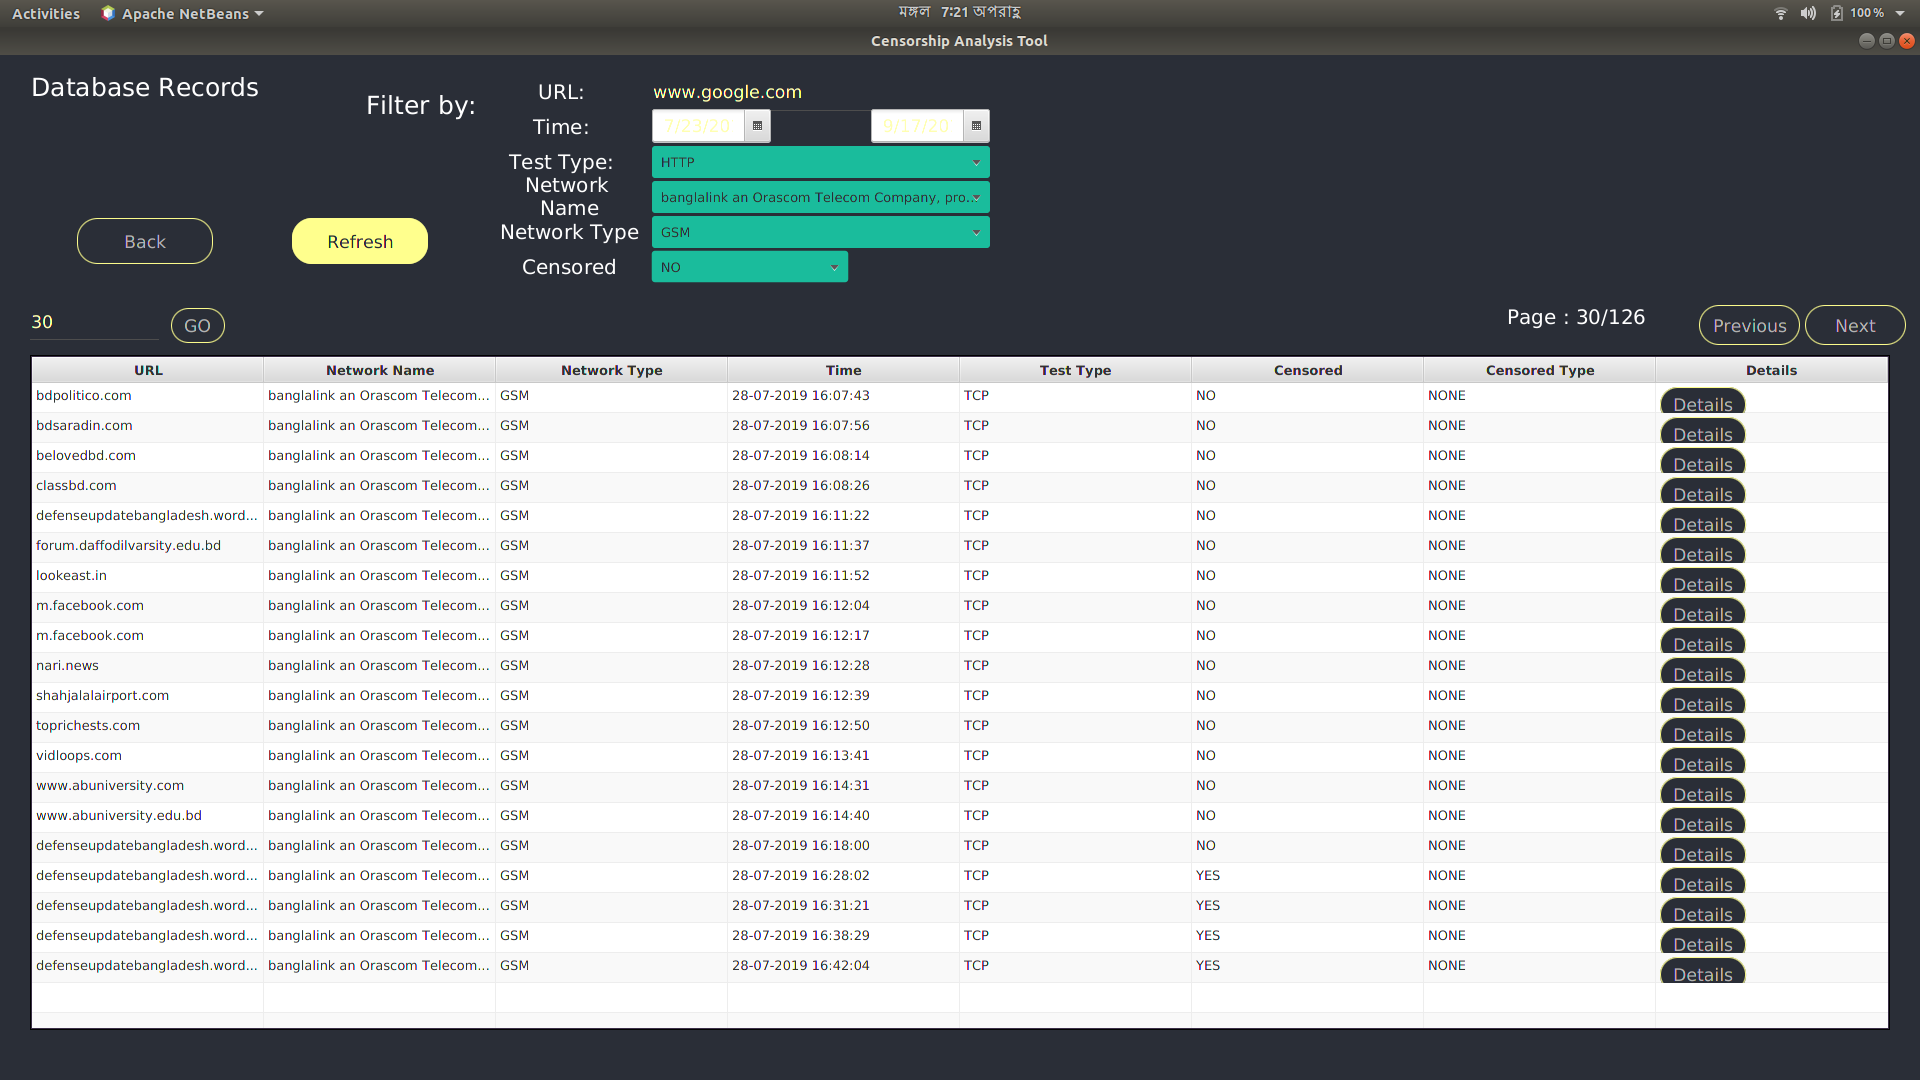
\includegraphics[width=\textwidth]{usersite/5beforefilter.png}
    \caption{Before applying filter}
    \label{fig:user5}
\end{figure}

\begin{figure}[h]
    \centering
    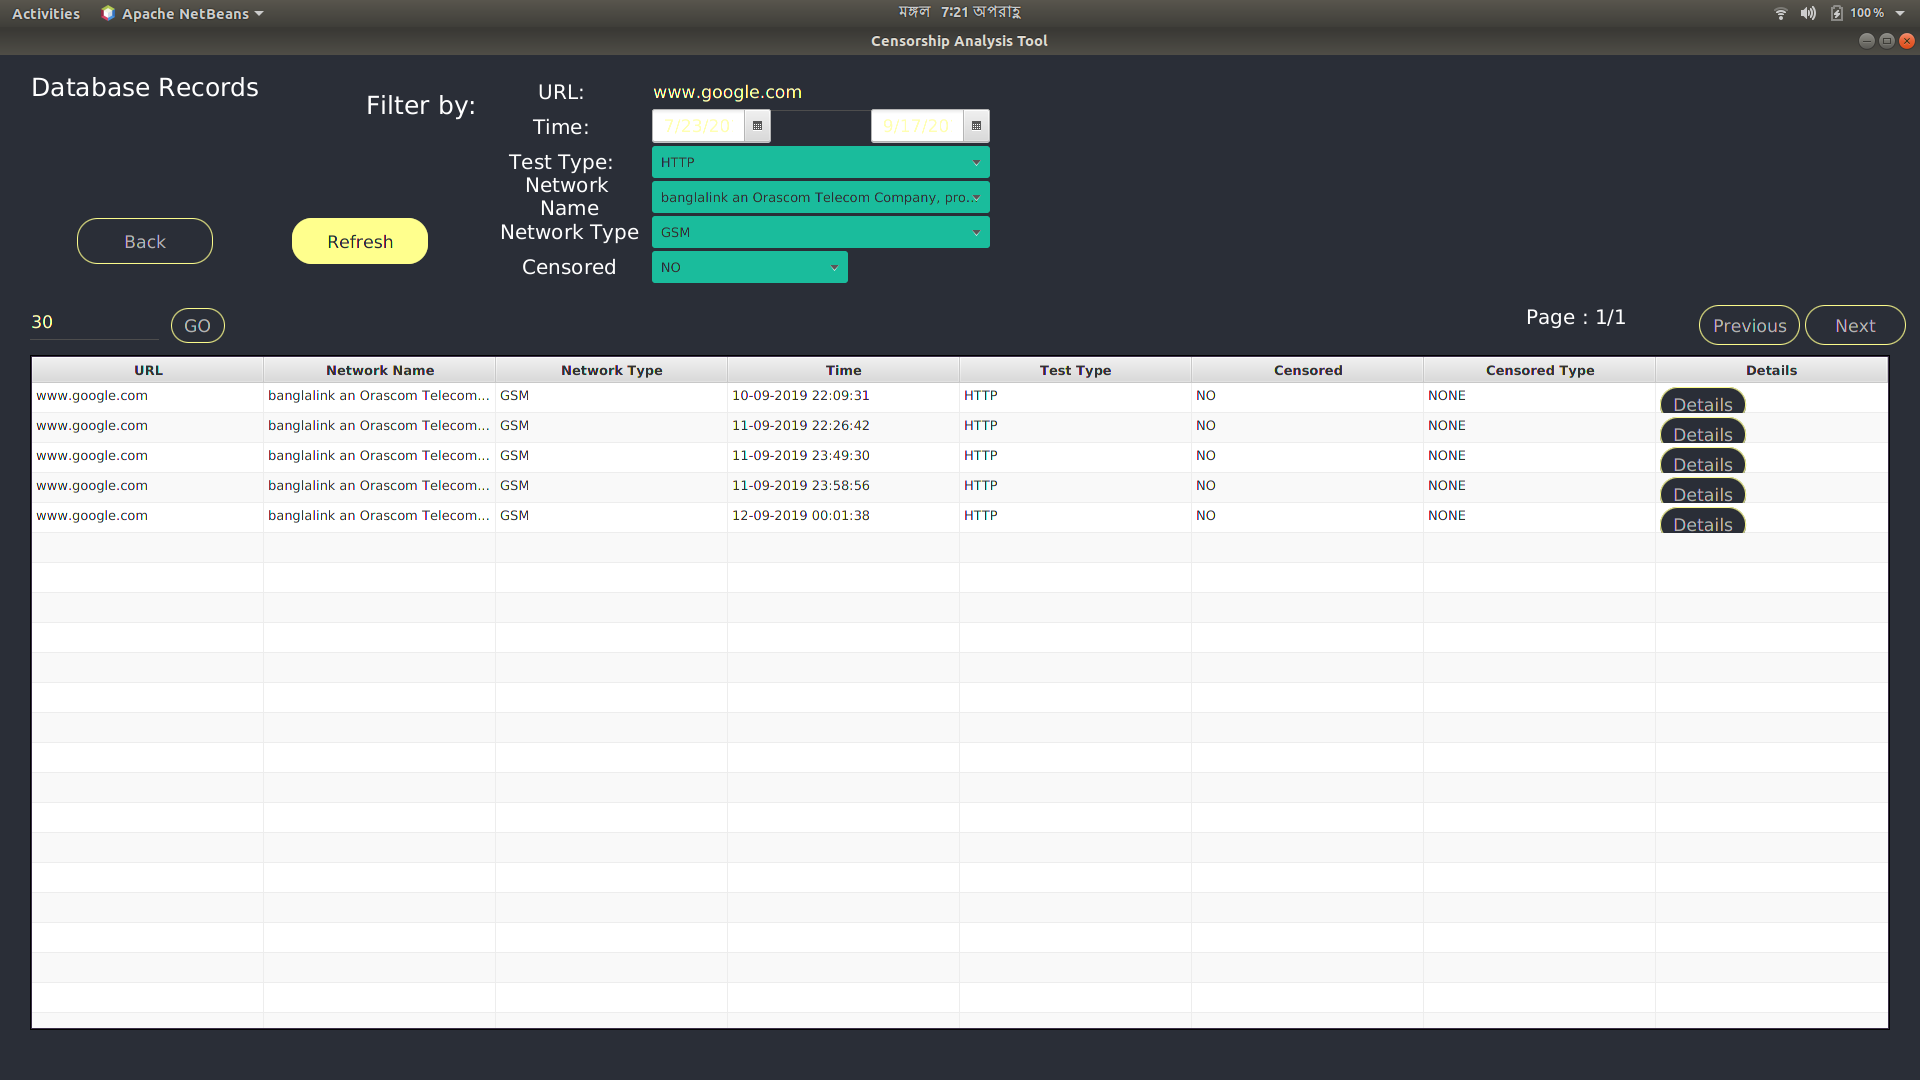
\includegraphics[width=\textwidth]{usersite/6afterfilter.png}
    \caption{After applying various filter}
    \label{fig:user6}
\end{figure}

After clicking \emph{Back} button, a user can come to home page again. 
\begin{figure}[h]
    \centering
    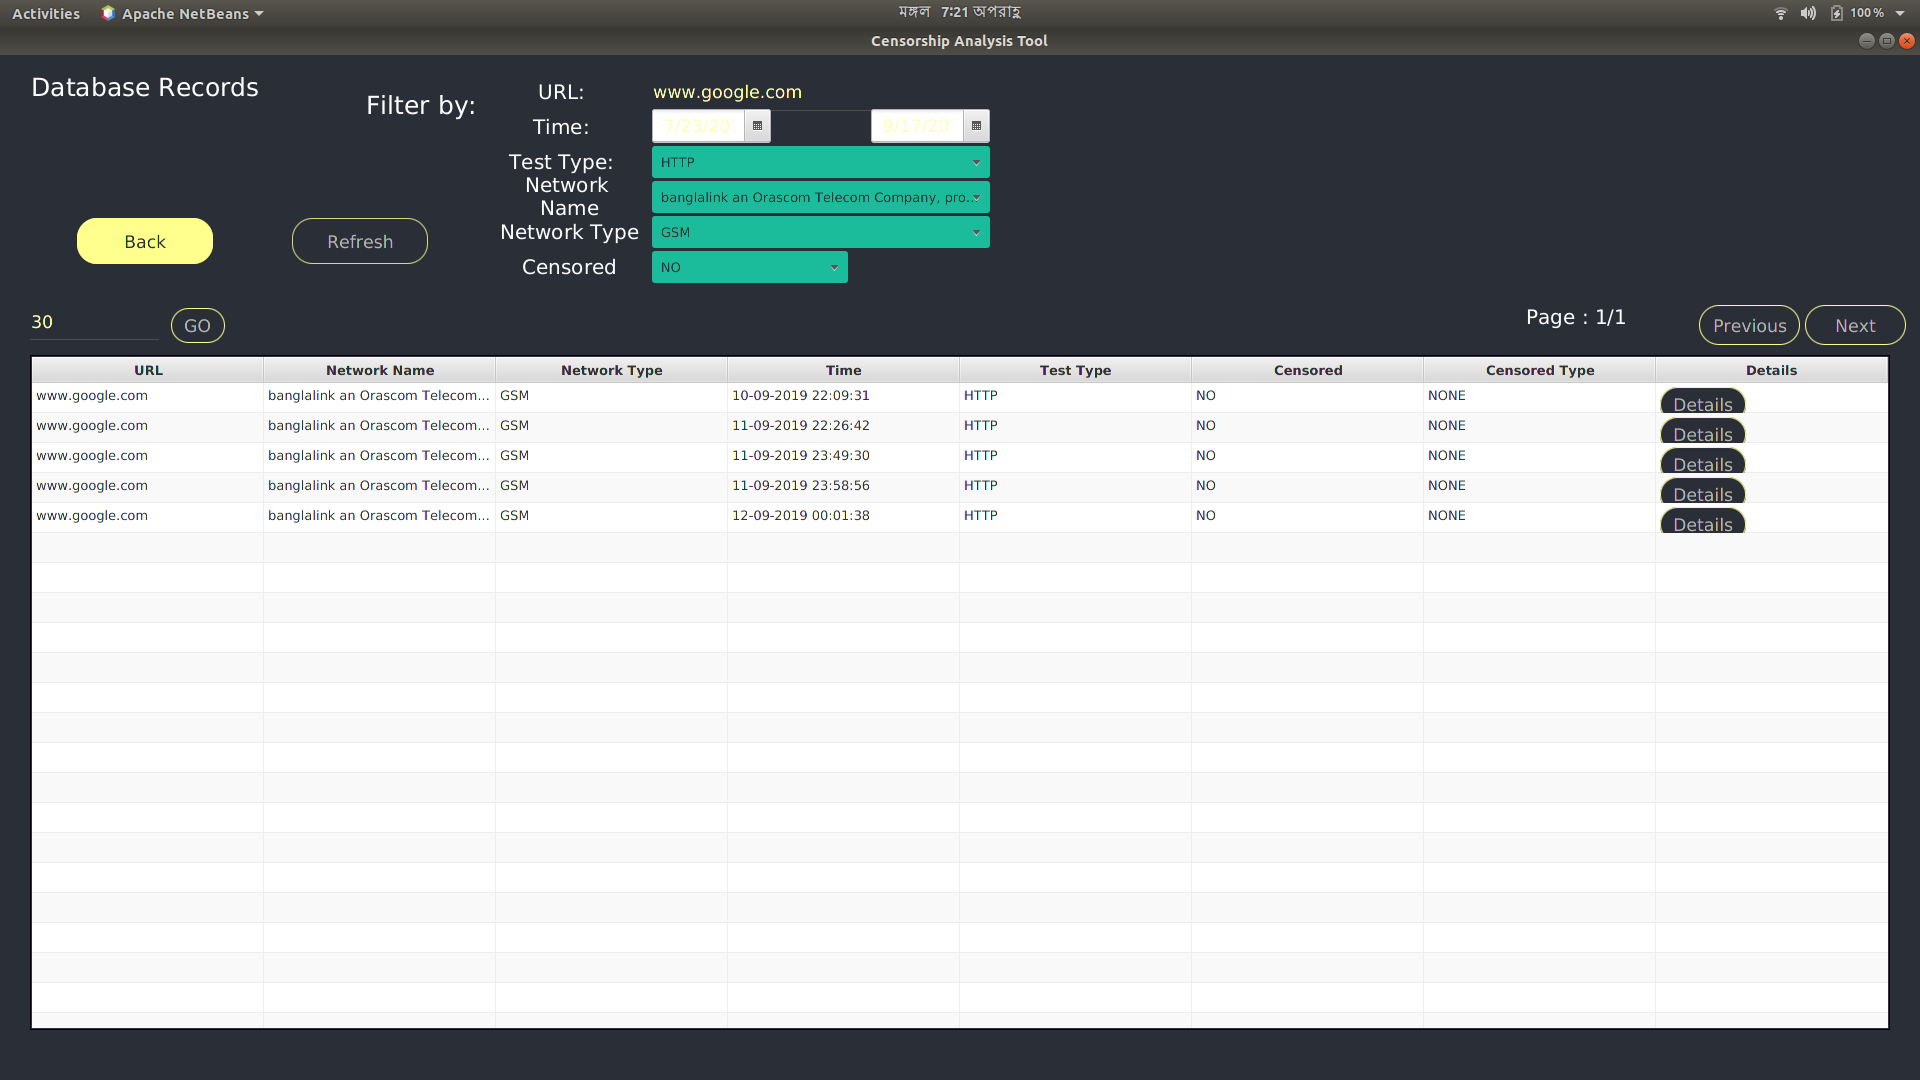
\includegraphics[width=\textwidth]{usersite/7back.png}
    \caption{Clicking back button}
    \label{fig:user7}
\end{figure}

\begin{figure}[h]
    \centering
    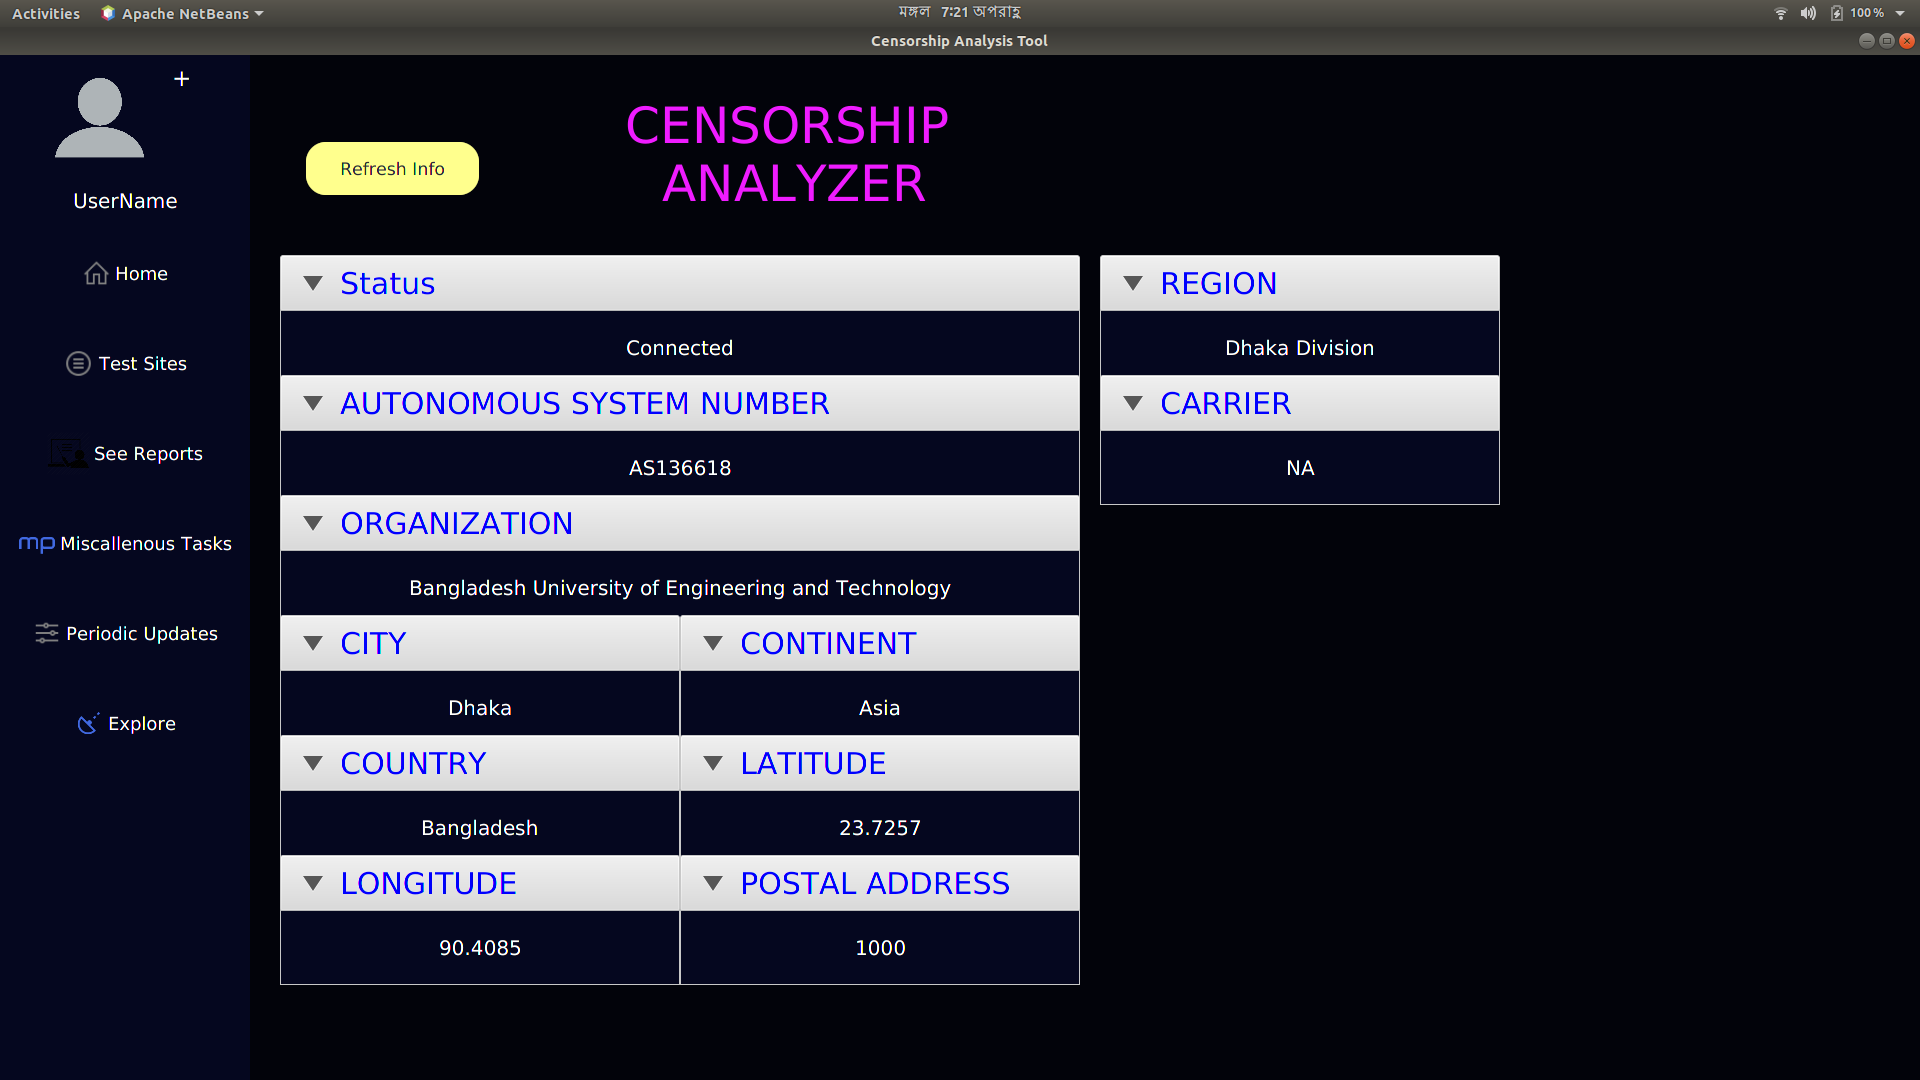
\includegraphics[width=\textwidth]{usersite/8homepage.png}
    \caption{Home page back}
    \label{fig:user8}
\end{figure}

After clicking \emph{Test Sites} a user should test single url or files of url by clicking file selector, selecting type of test and accepting all terms and condition submit the test query. He can see file's data by clicking \emph{View File} button.
\begin{figure}[h]
    \centering
    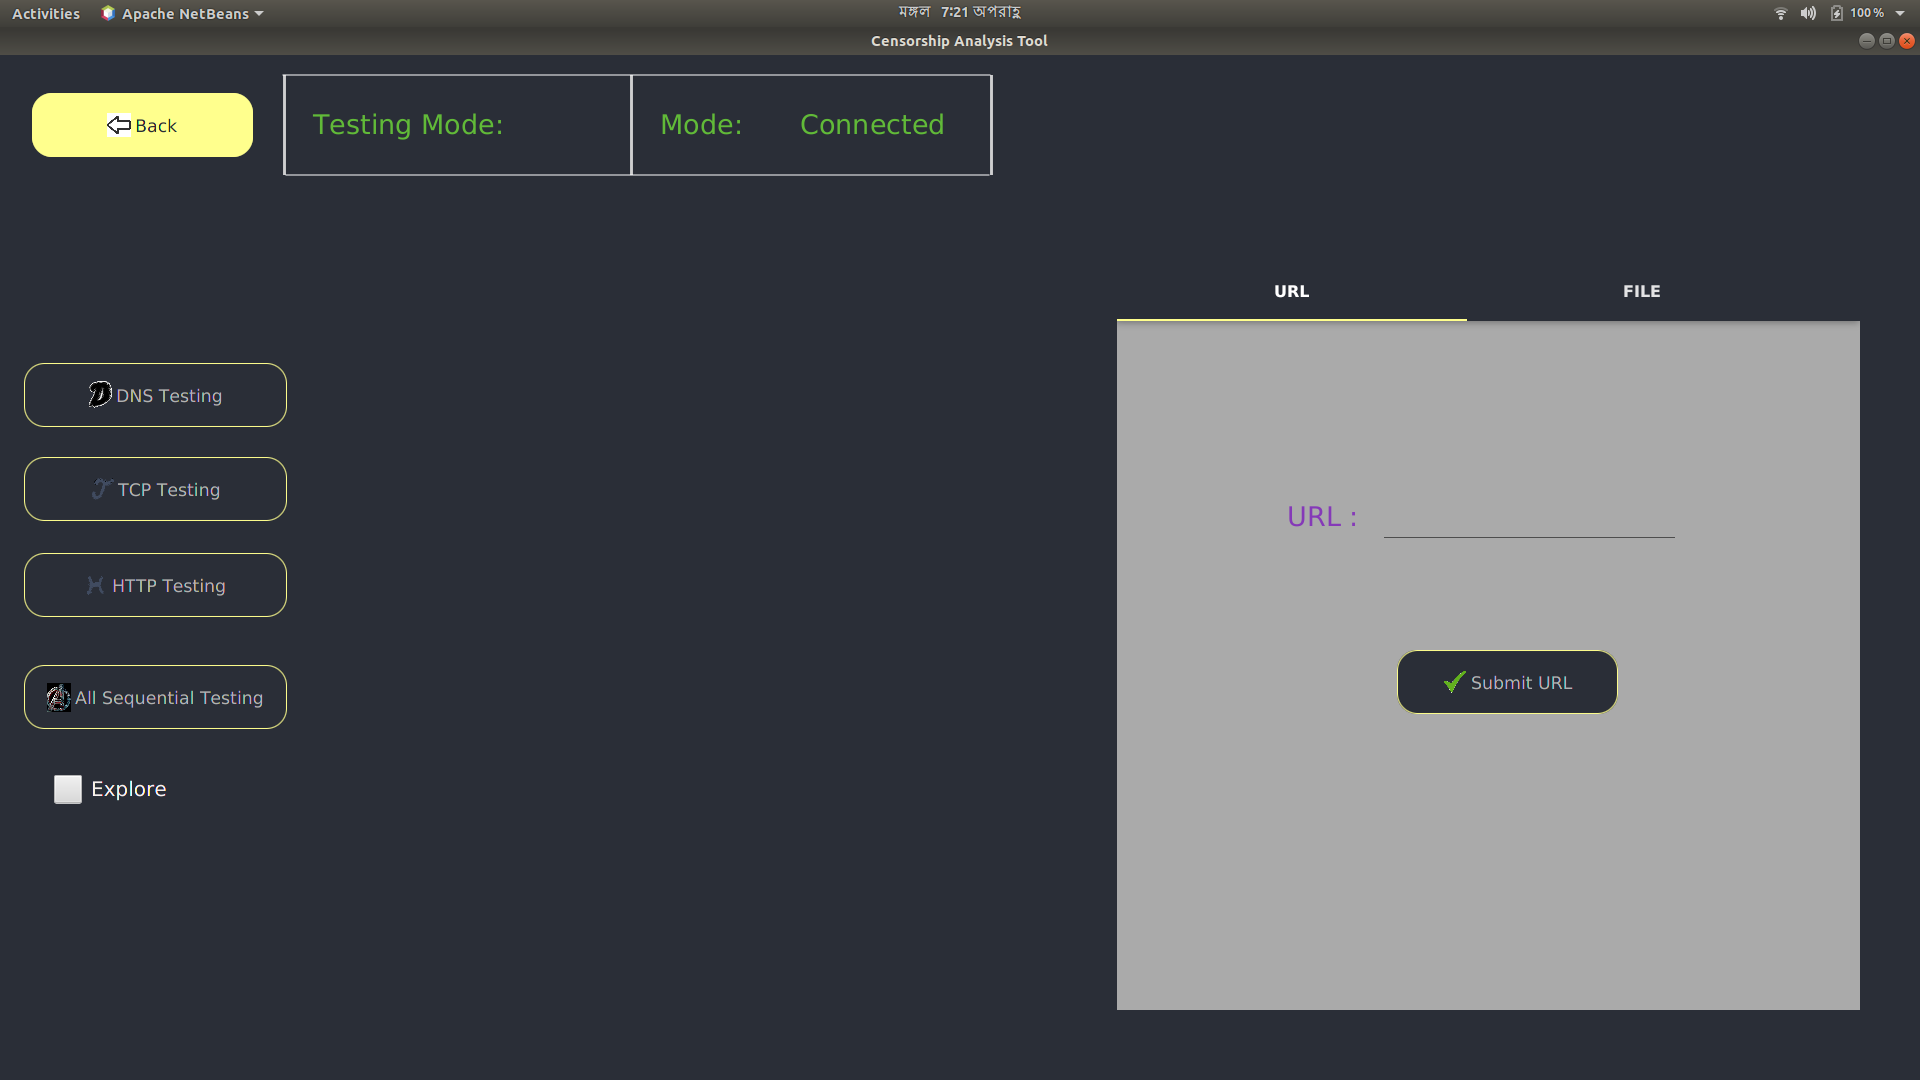
\includegraphics[width=\textwidth]{usersite/9dnstest.png}
    \caption{A sample testing window}
    \label{fig:user9}
\end{figure}

\begin{figure}[h]
    \centering
    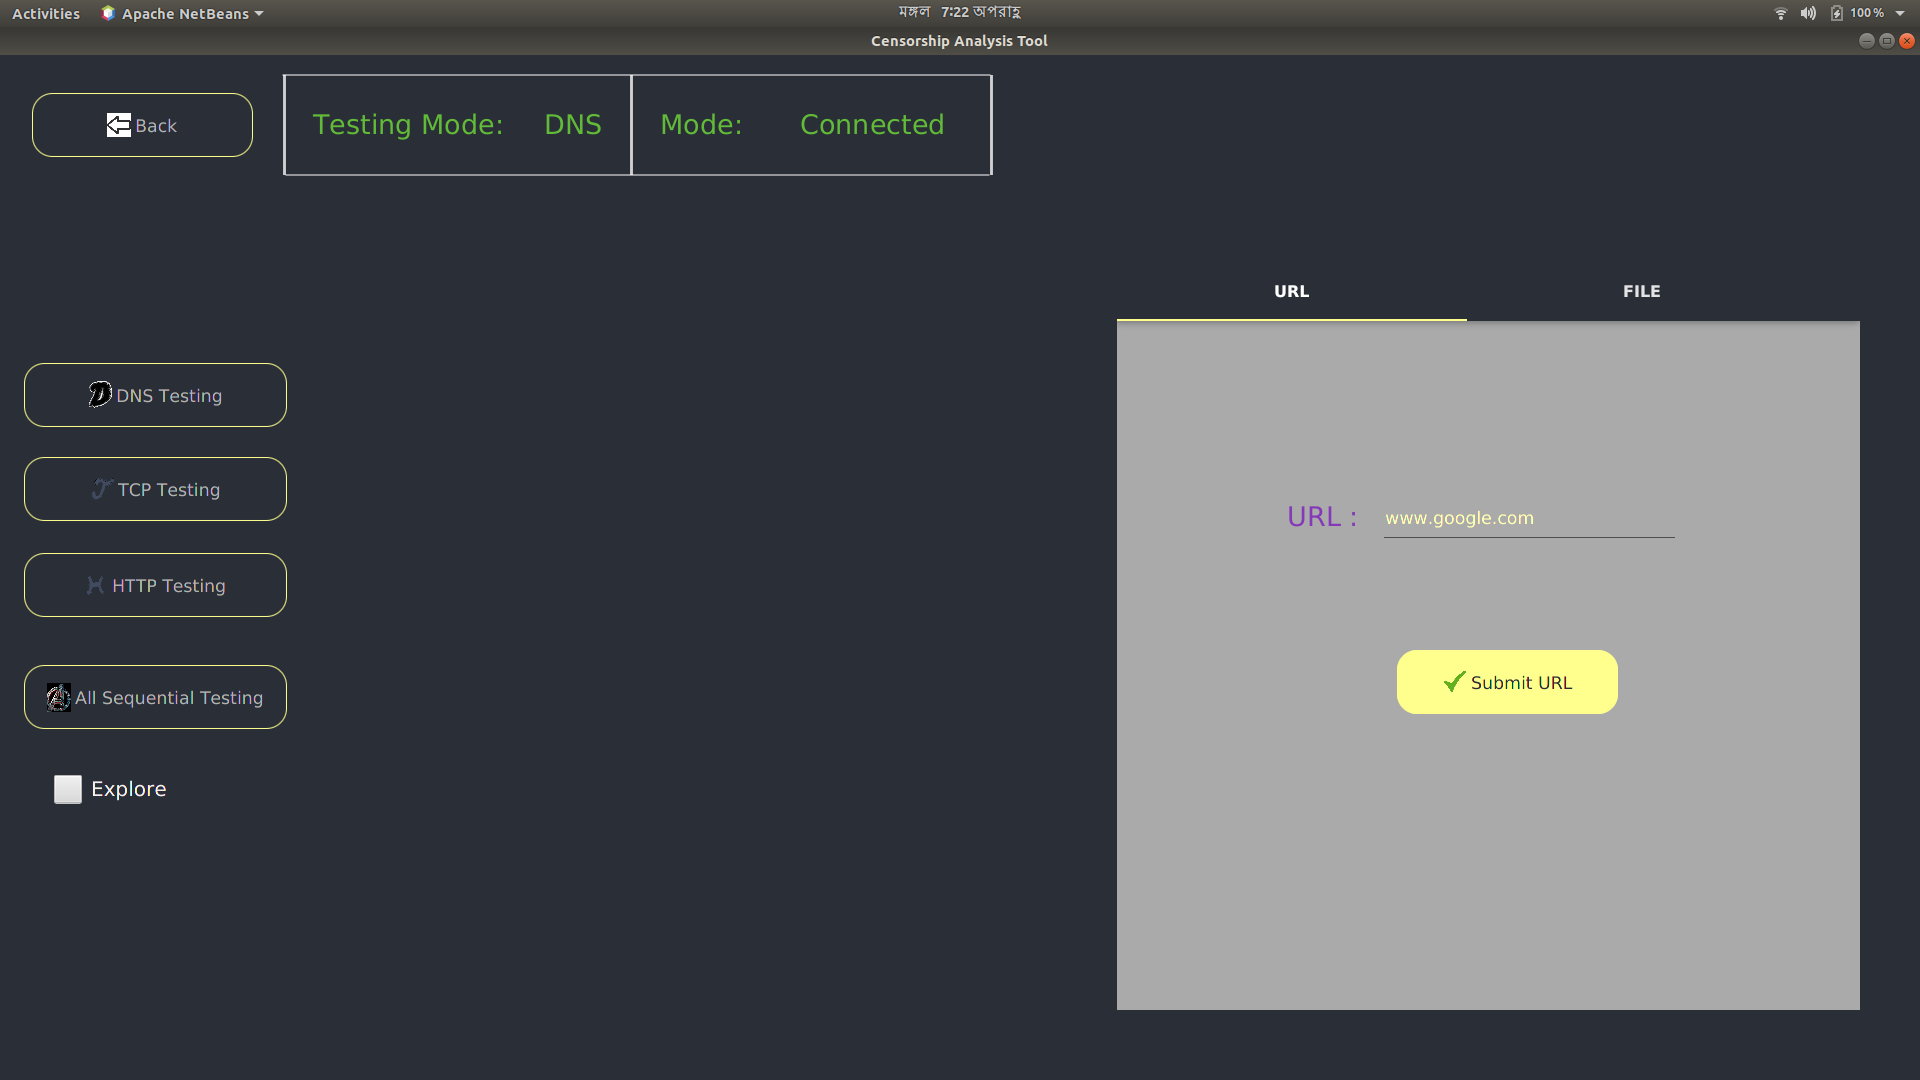
\includegraphics[width=\textwidth]{usersite/10input.png}
    \caption{Another dns test input}
    \label{fig:user10}
\end{figure}


\begin{figure}[h]
    \centering
    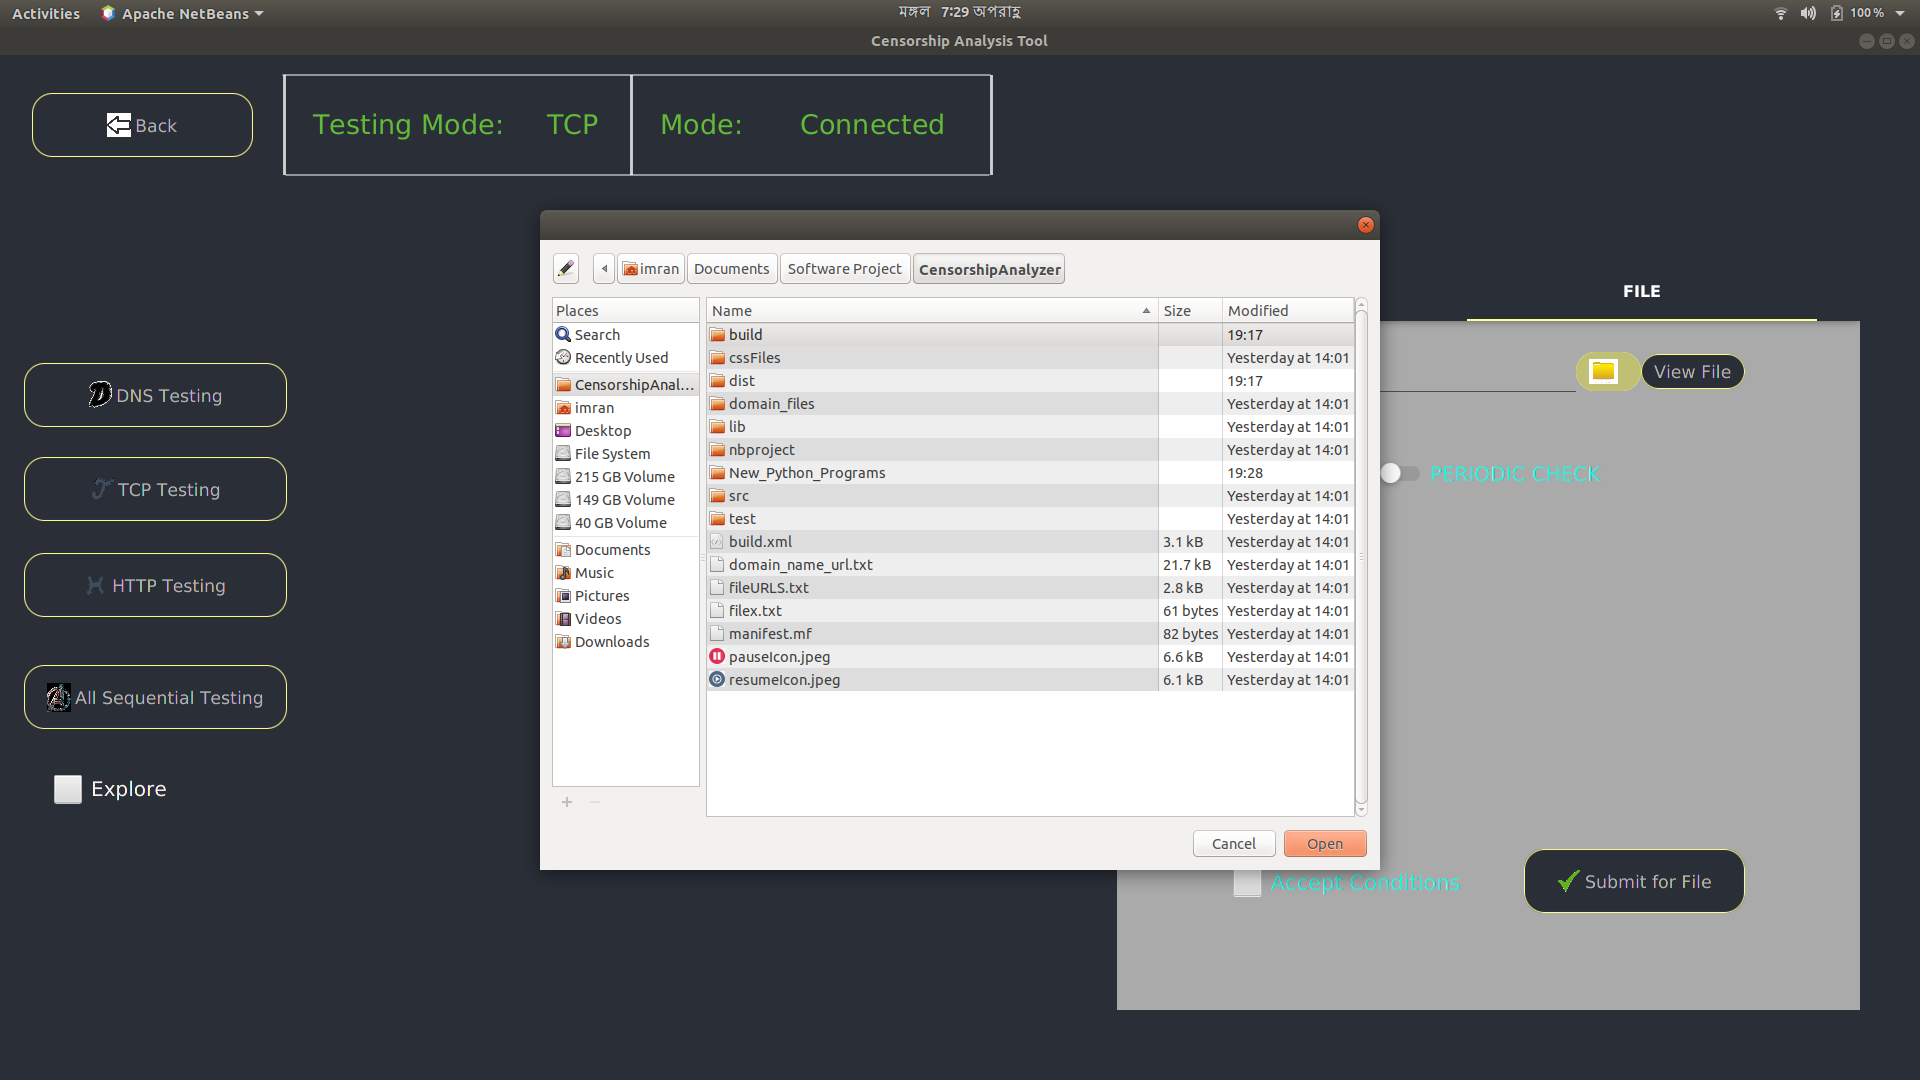
\includegraphics[width=\textwidth]{usersite/26selectfiles.png}
    \caption{File with urls can be selected to test}
    \label{fig:user25}
\end{figure}


\begin{figure}[h]
    \centering
    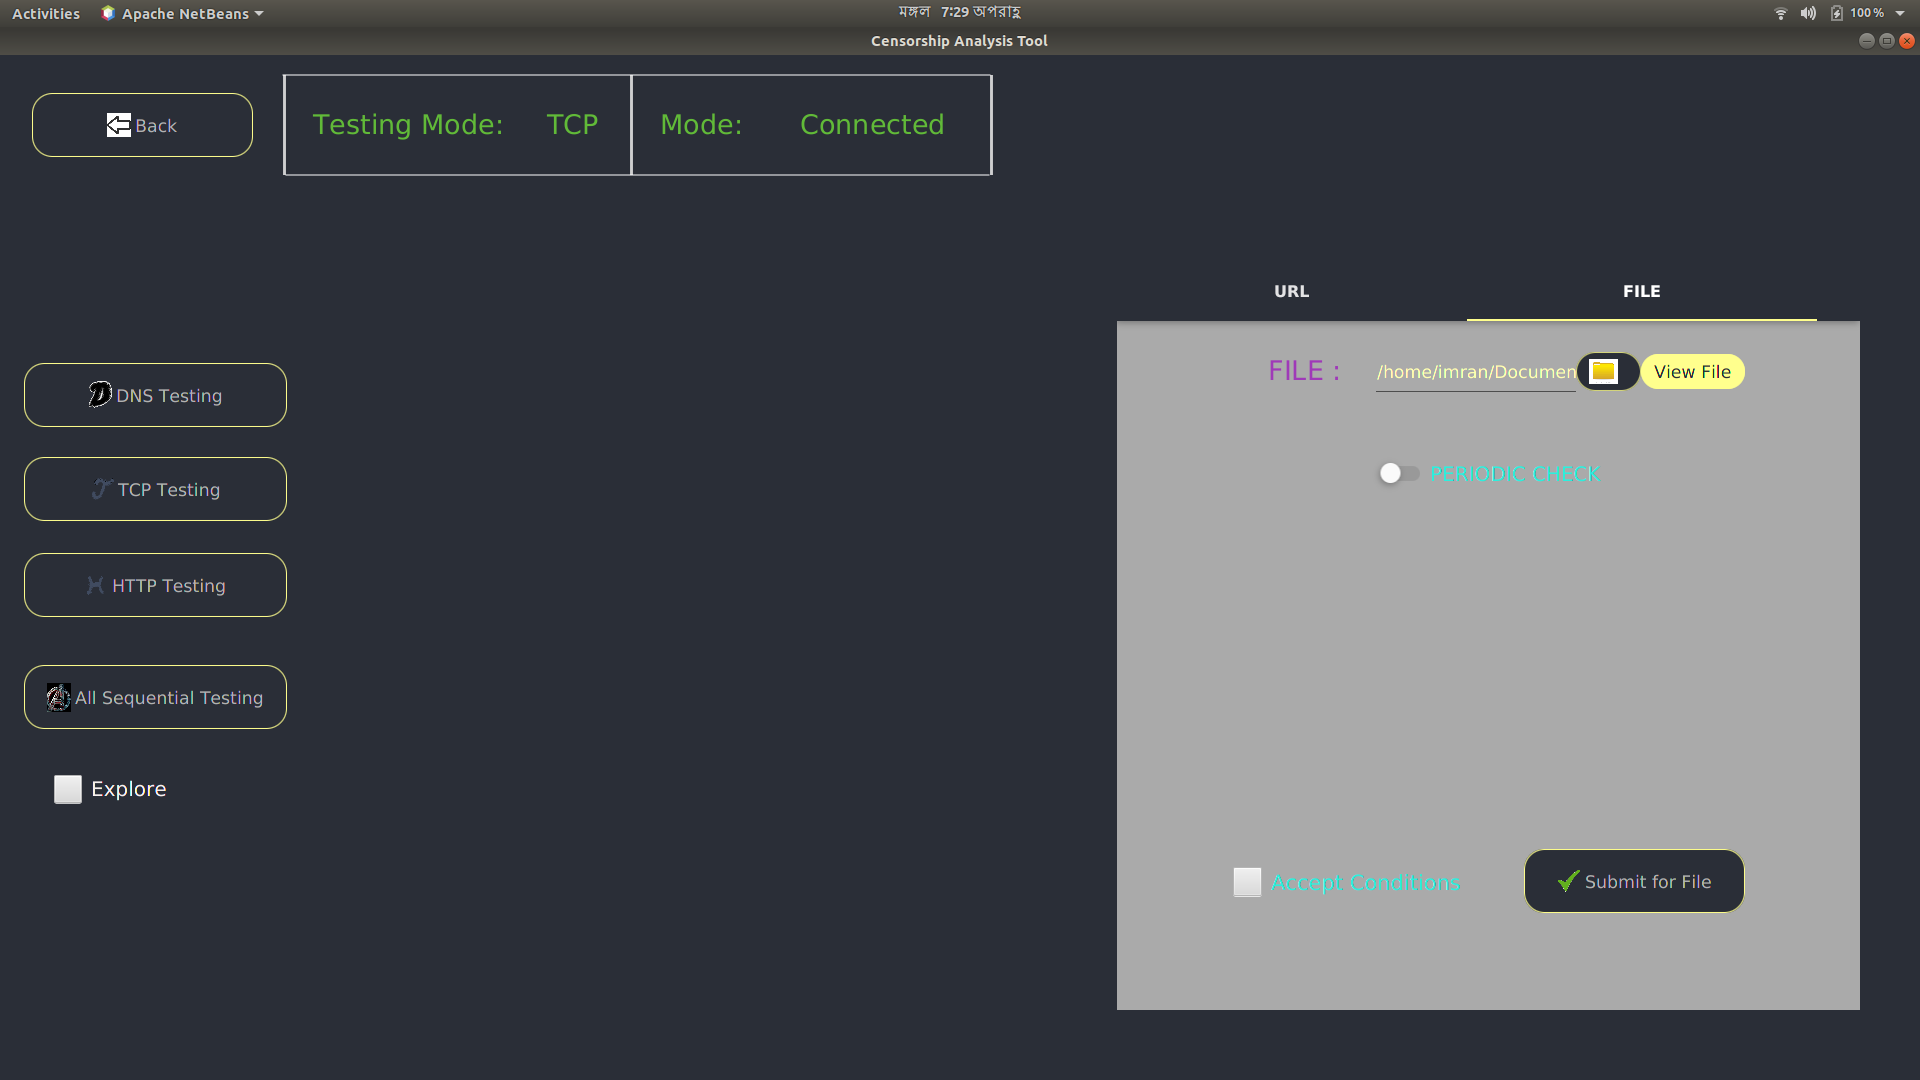
\includegraphics[width=\textwidth]{usersite/27inputfile2.png}
    \caption{Selected file url is seen}
    \label{fig:user26}
\end{figure}

\begin{figure}[h]
    \centering
    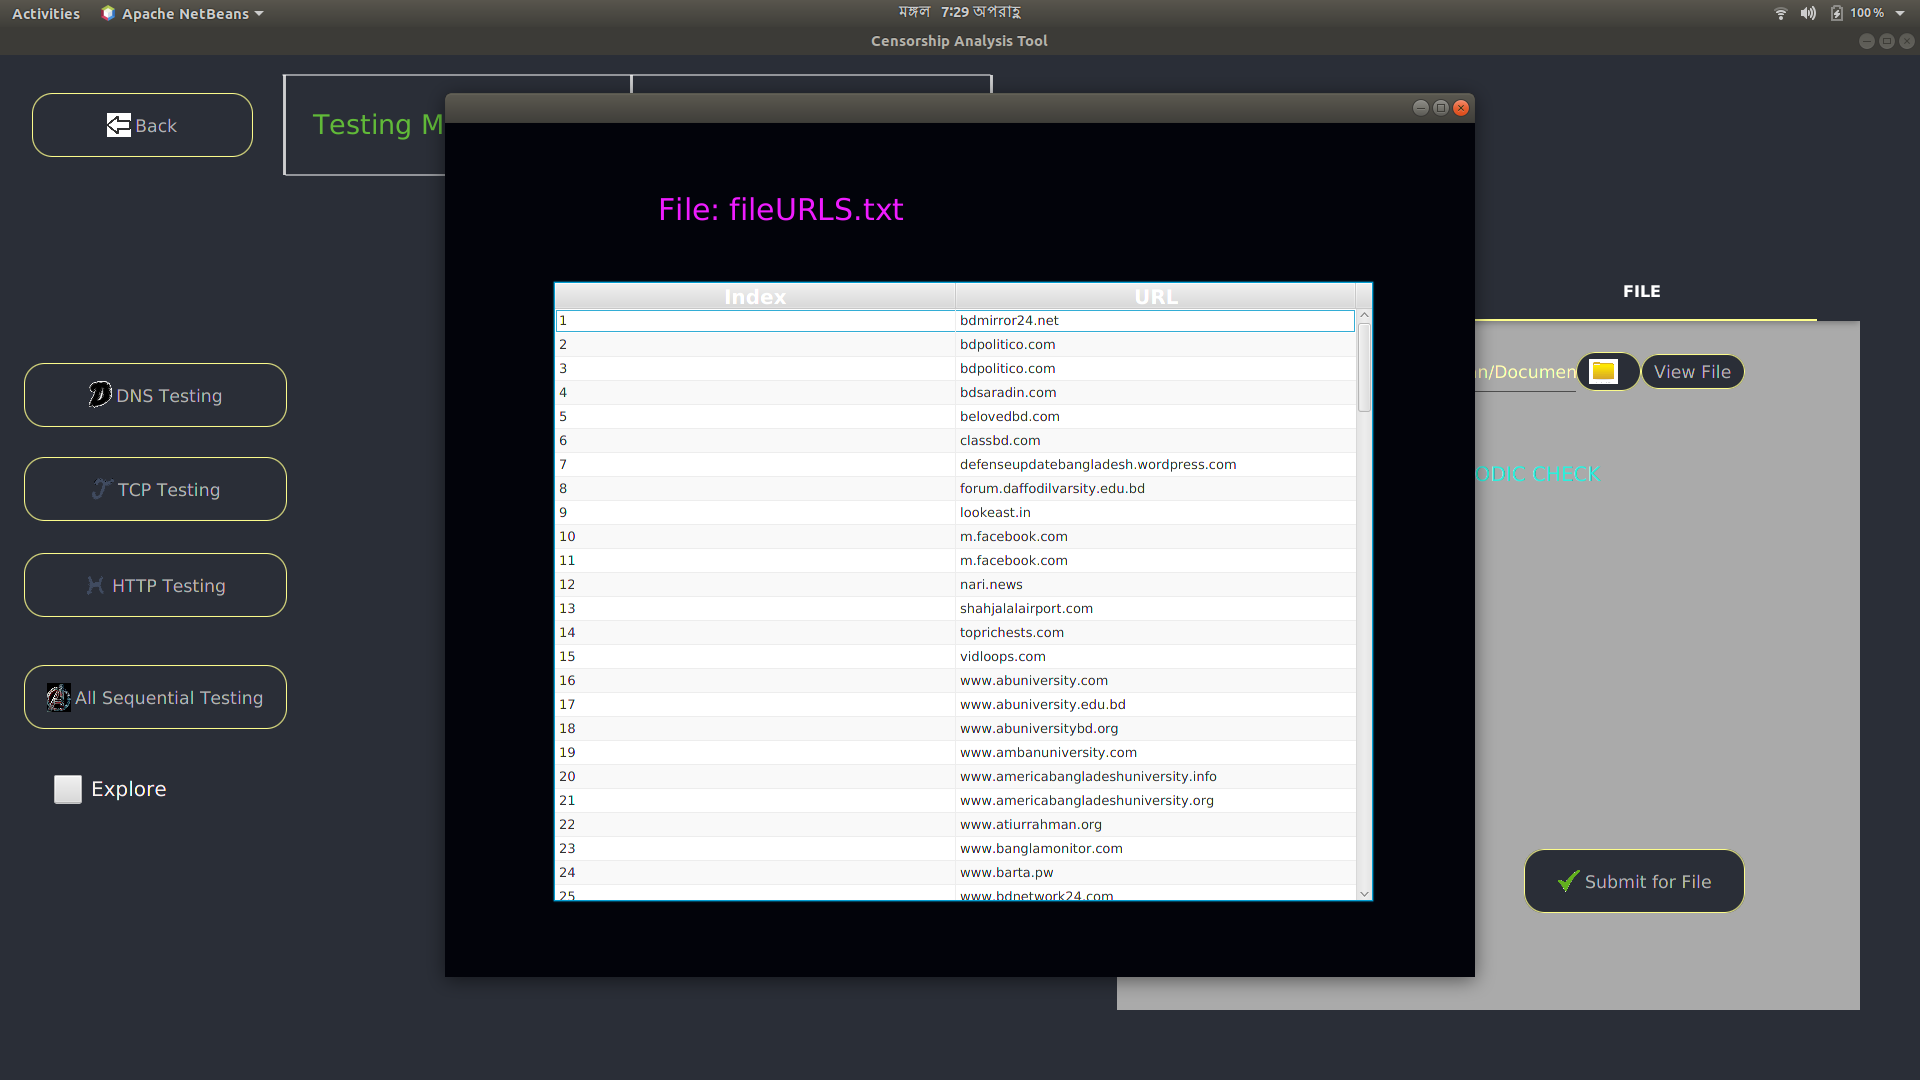
\includegraphics[width=\textwidth]{usersite/28fileread.png}
    \caption{File's url can be seen}
    \label{fig:user27}
\end{figure}



\begin{figure}[h]
    \centering
    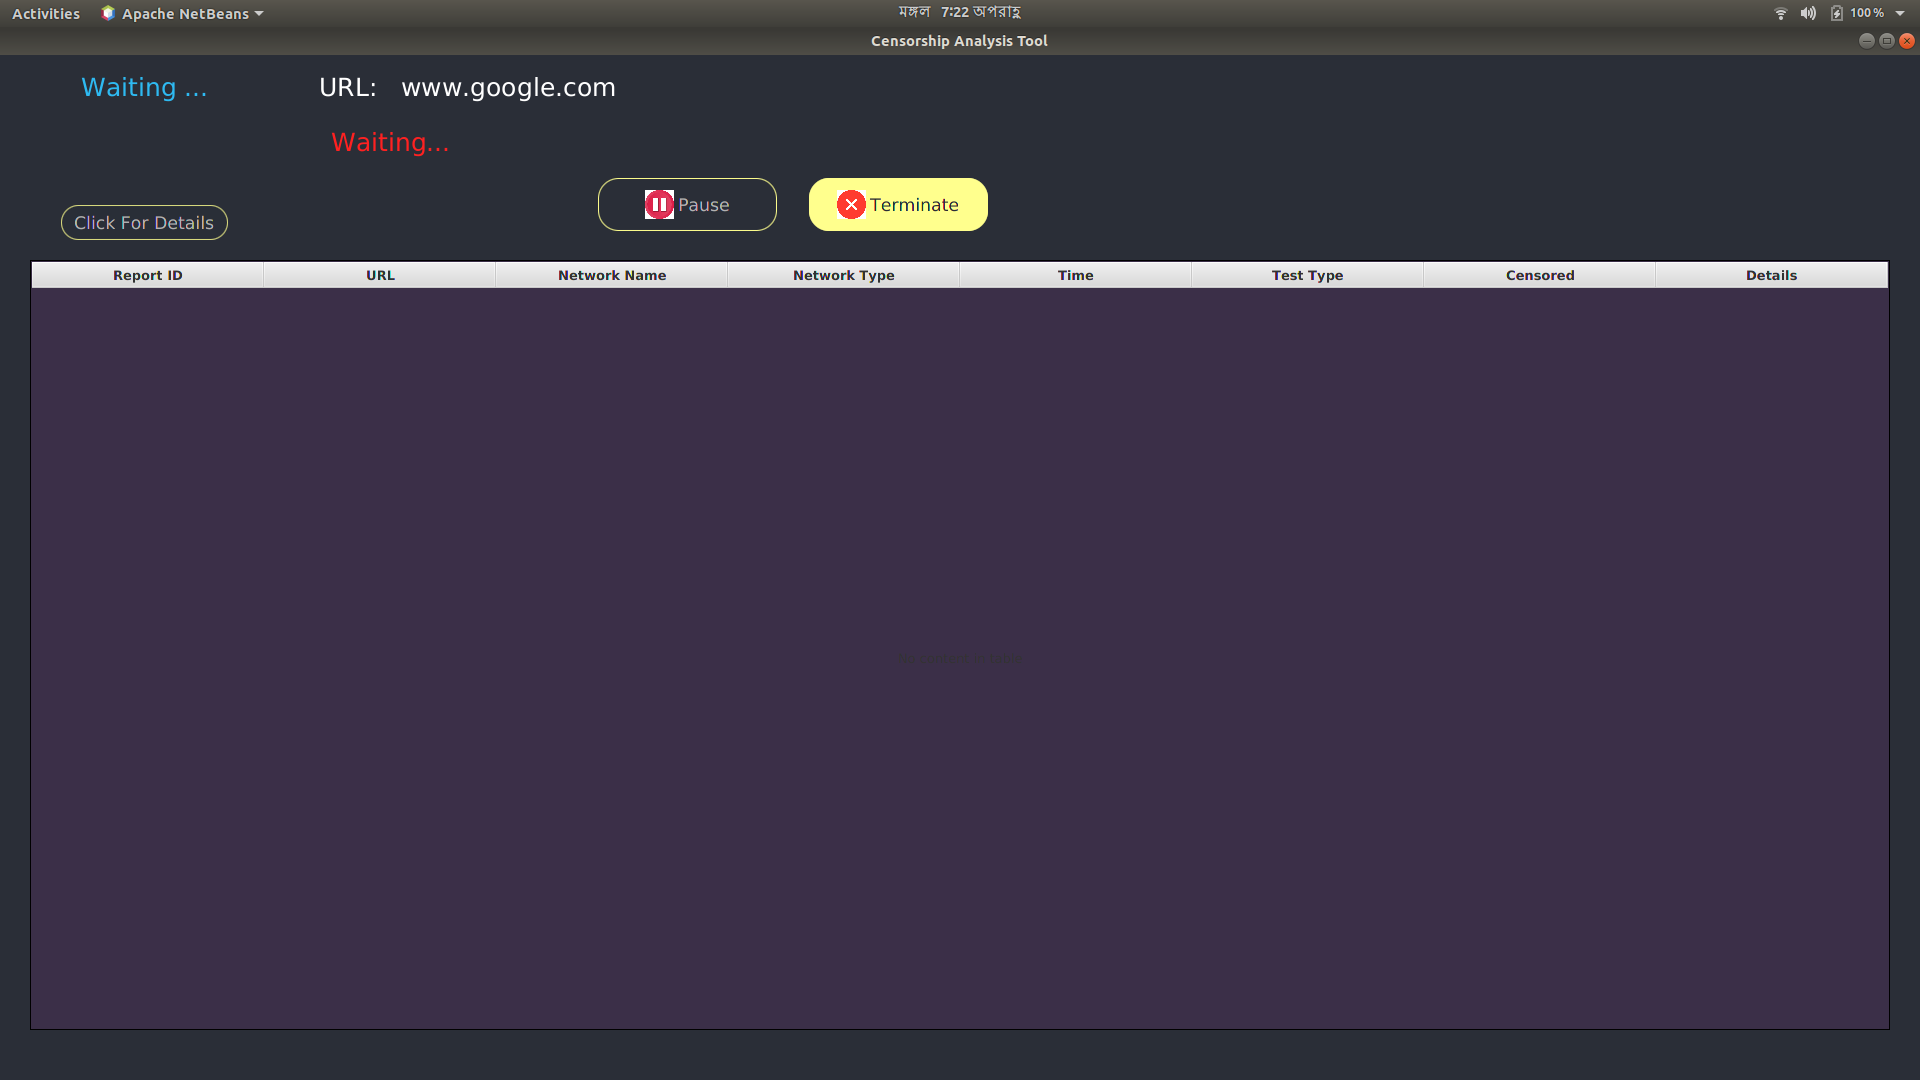
\includegraphics[width=\textwidth]{usersite/11waiting.png}
    \caption{After inserting input of testing new dynamic window appeared}
    \label{fig:user11}
\end{figure}

A user can terminate or pause the testing by clicking \emph{Terminate} and \emph{Pause} button respectively.
\begin{figure}[h]
    \centering
    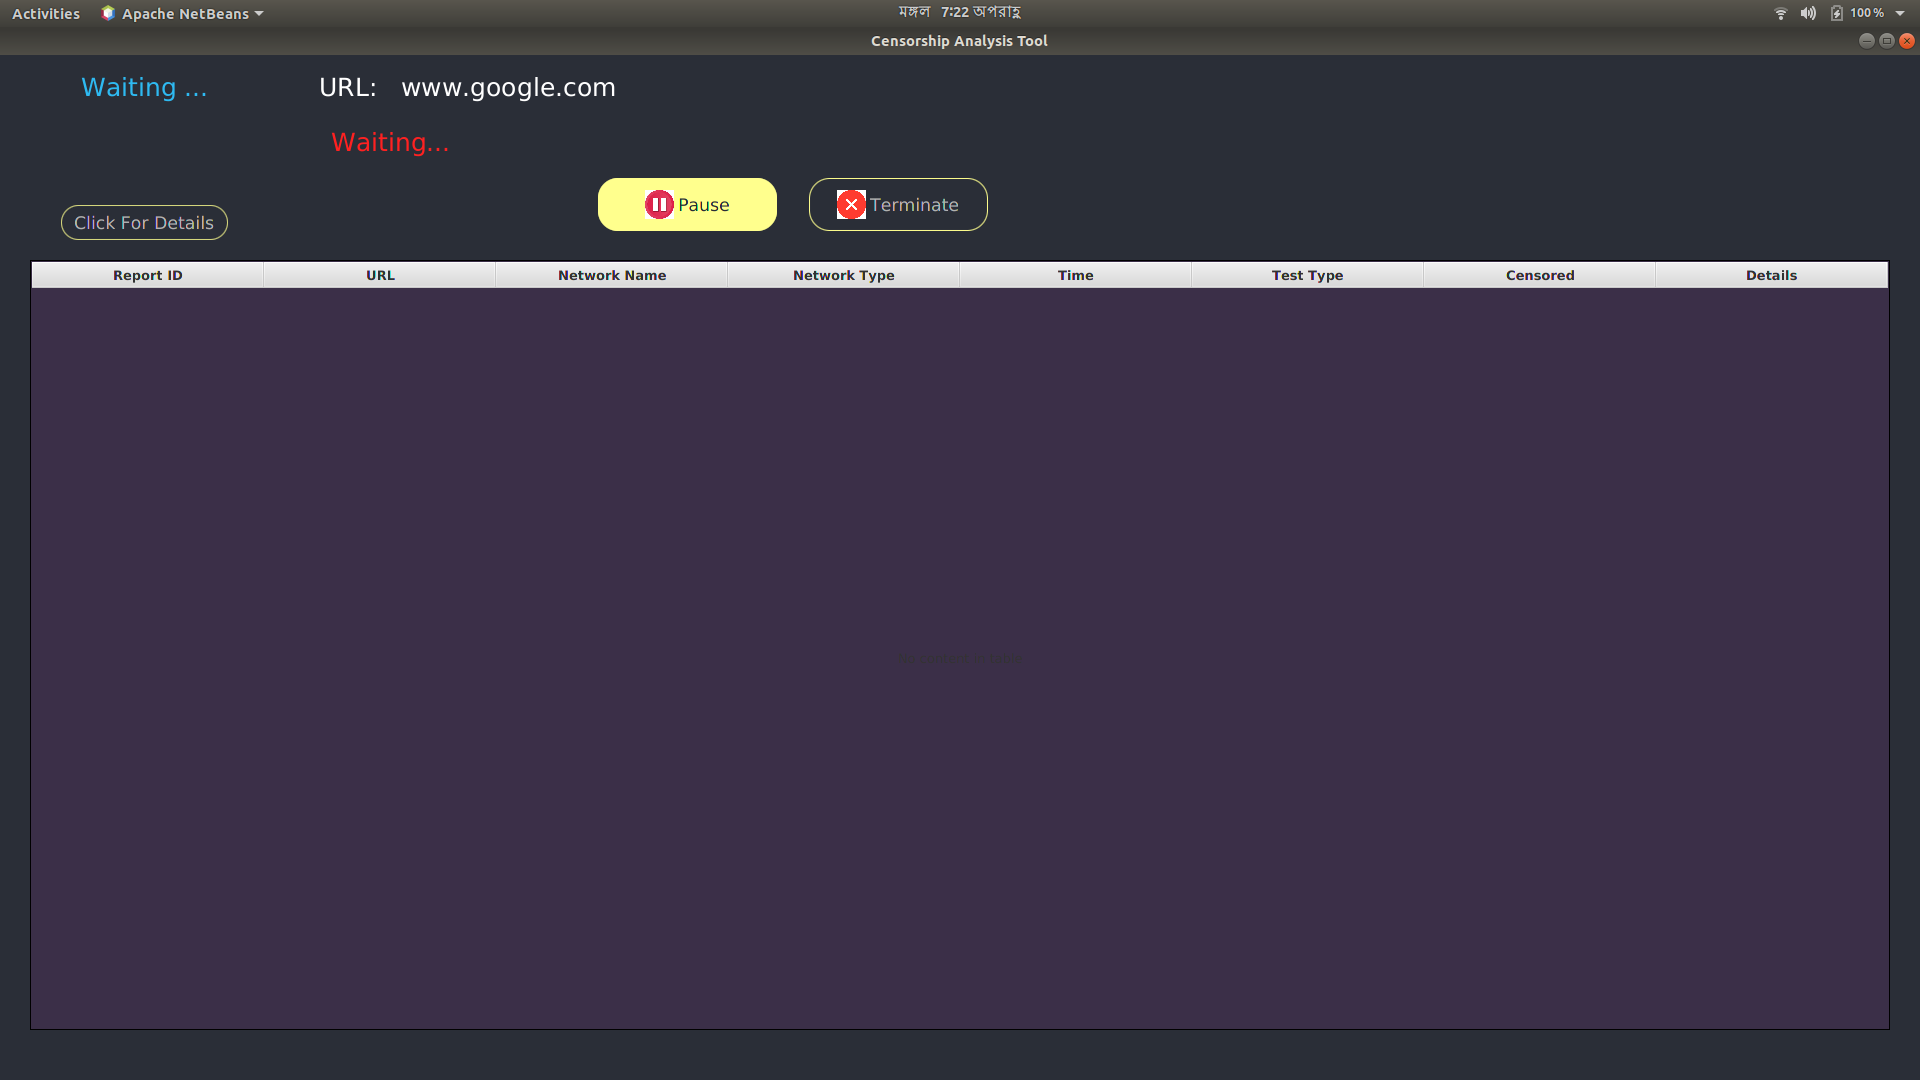
\includegraphics[width=\textwidth]{usersite/12pause.png}
    \caption{After clicking pause button}
    \label{fig:user12}
\end{figure}

\begin{figure}[h]
    \centering
    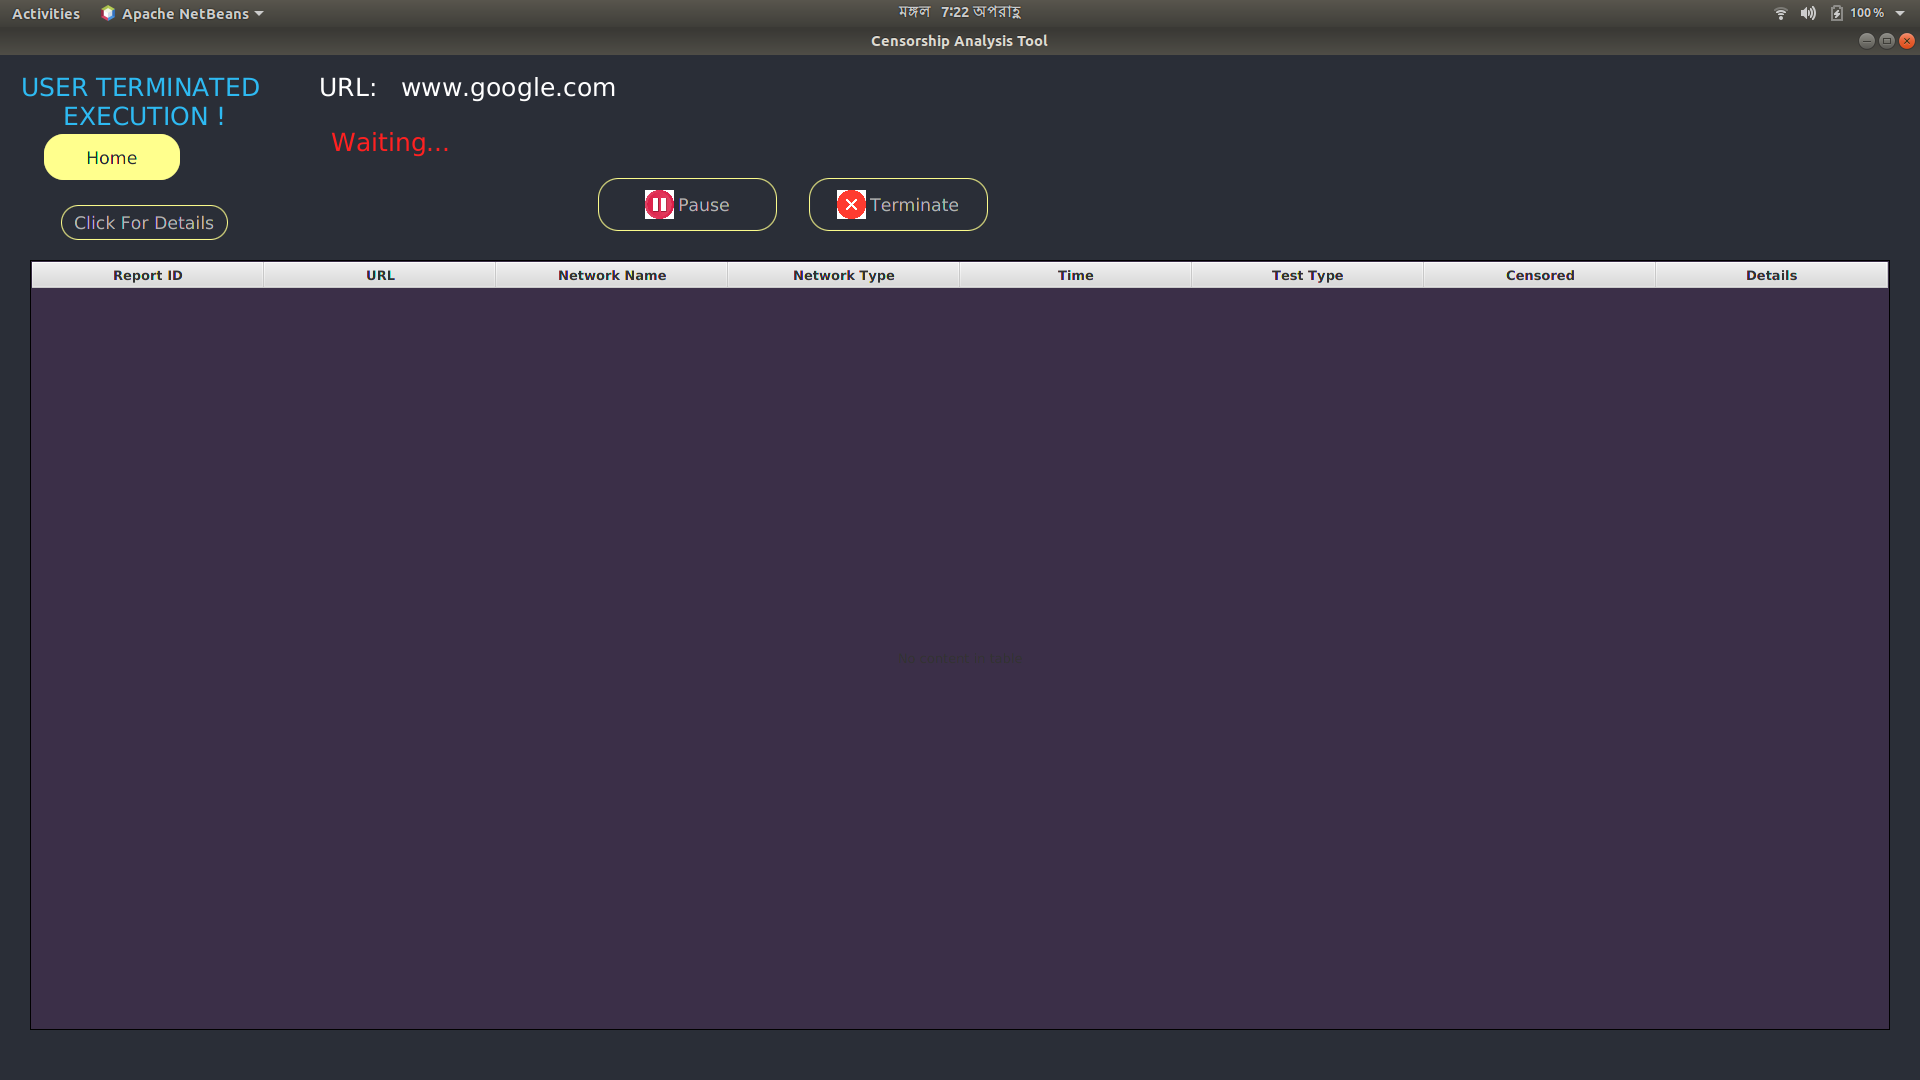
\includegraphics[width=\textwidth]{usersite/13paused.png}
    \caption{After clicking terminate button}
    \label{fig:user13}
\end{figure}

\begin{figure}[h]
    \centering
    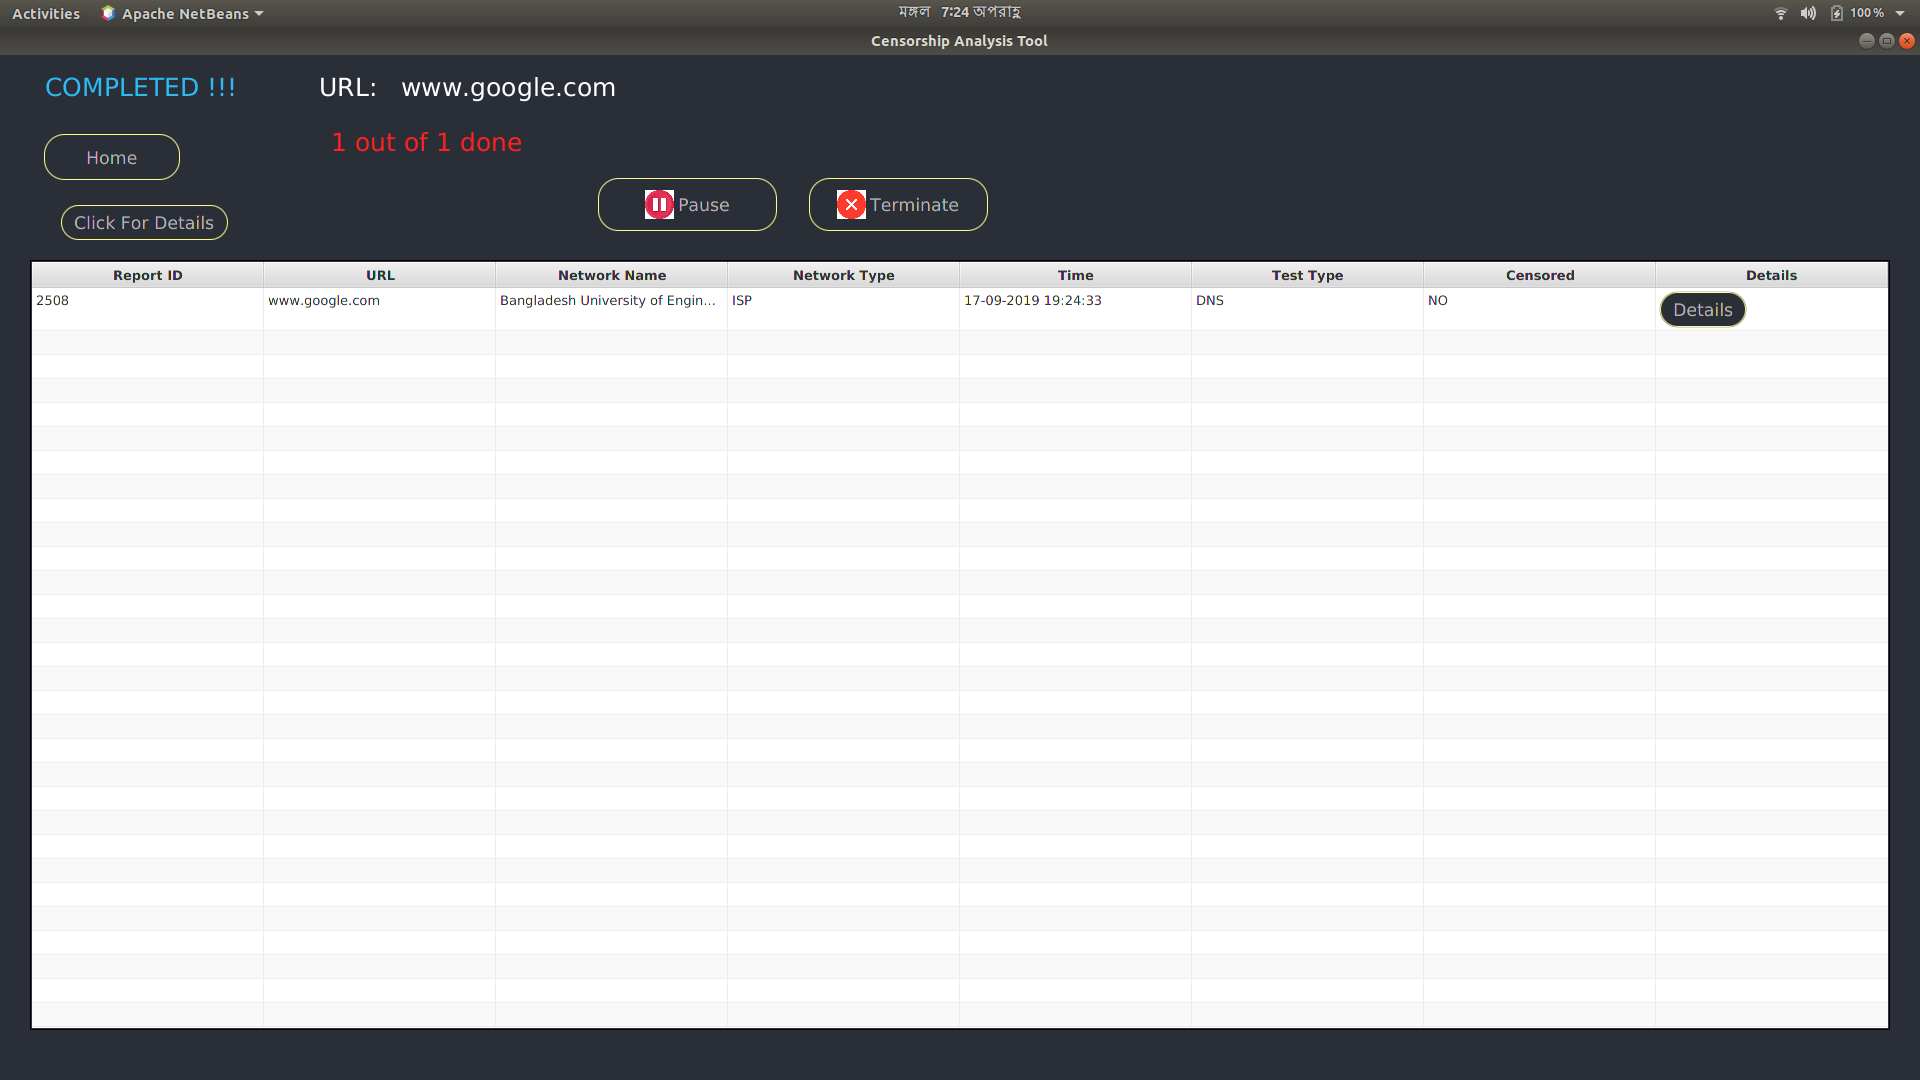
\includegraphics[width=\textwidth]{usersite/14completed.png}
    \caption{After completion of 1 test}
    \label{fig:user14}
\end{figure}

\begin{figure}[h]
    \centering
    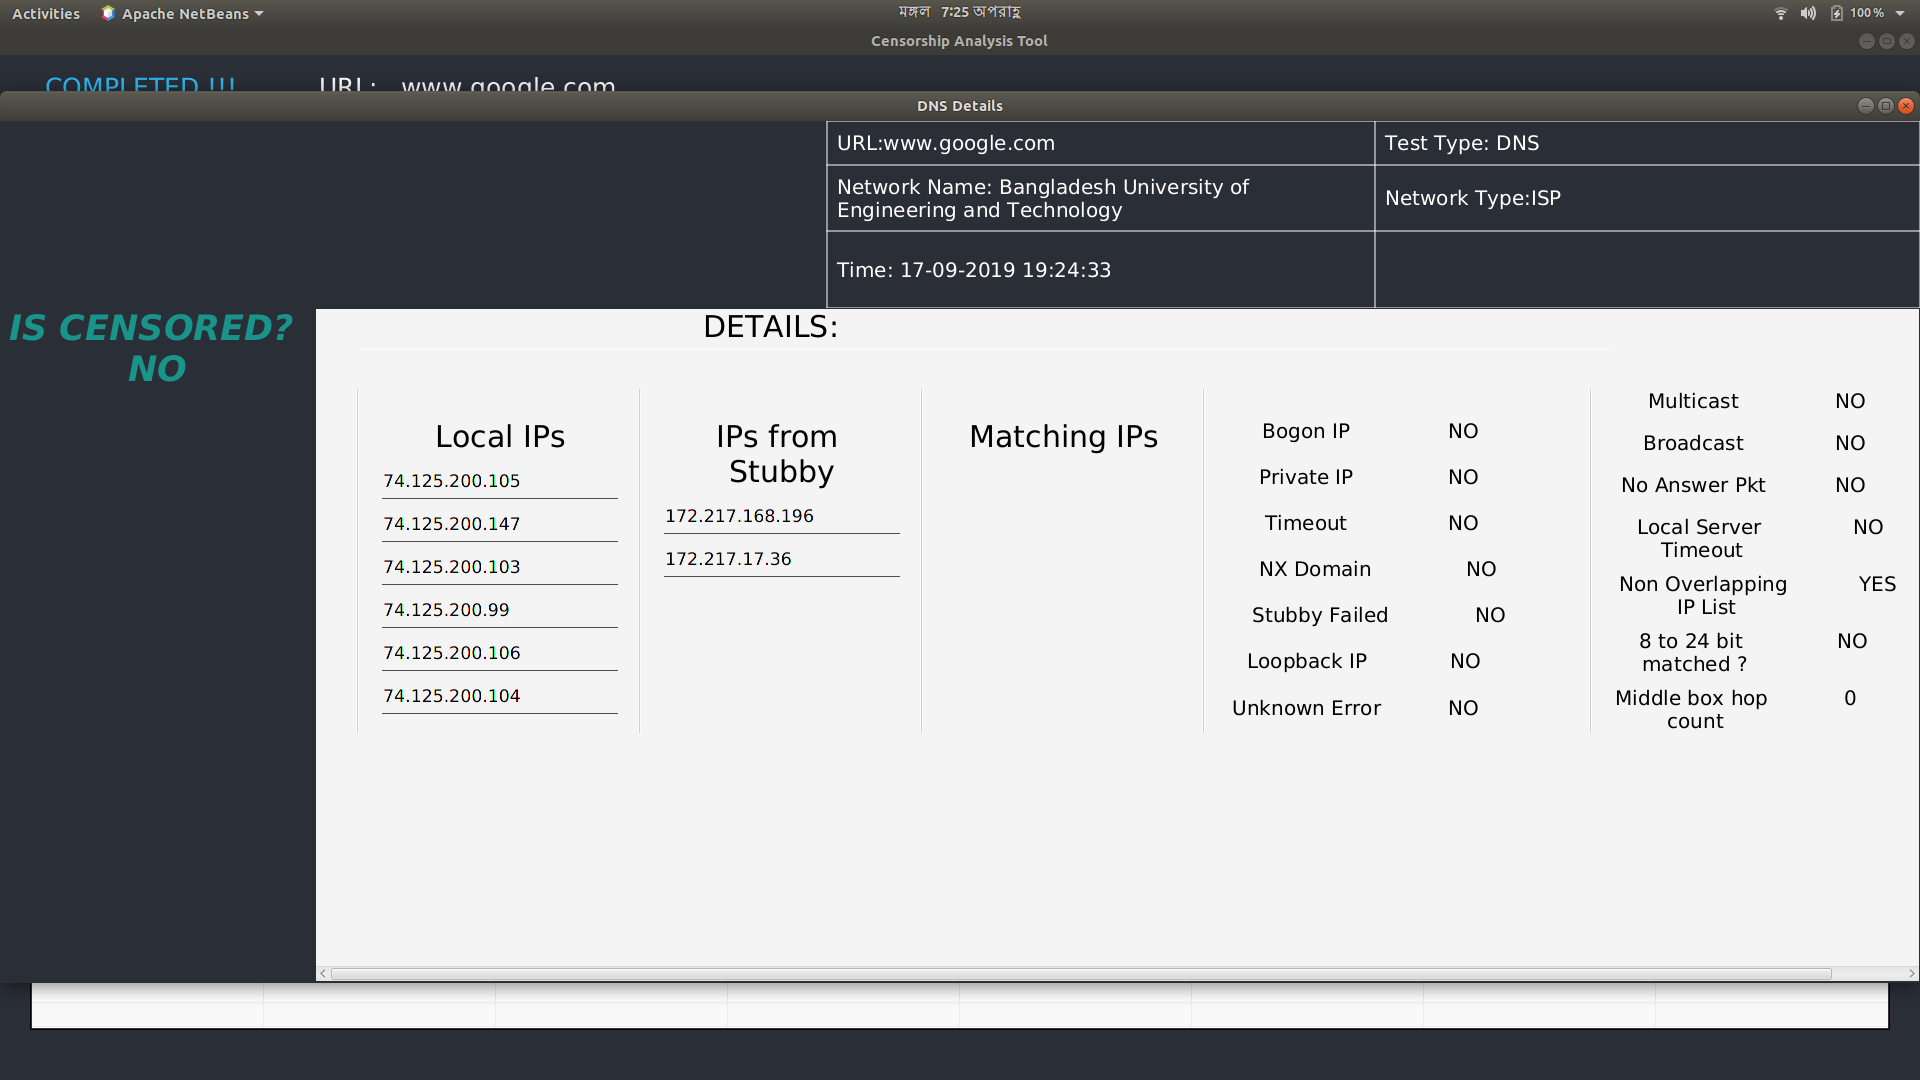
\includegraphics[width=\textwidth]{usersite/15details.png}
    \caption{After clicking details button}
    \label{fig:user15}
\end{figure}

\begin{figure}[h]
    \centering
    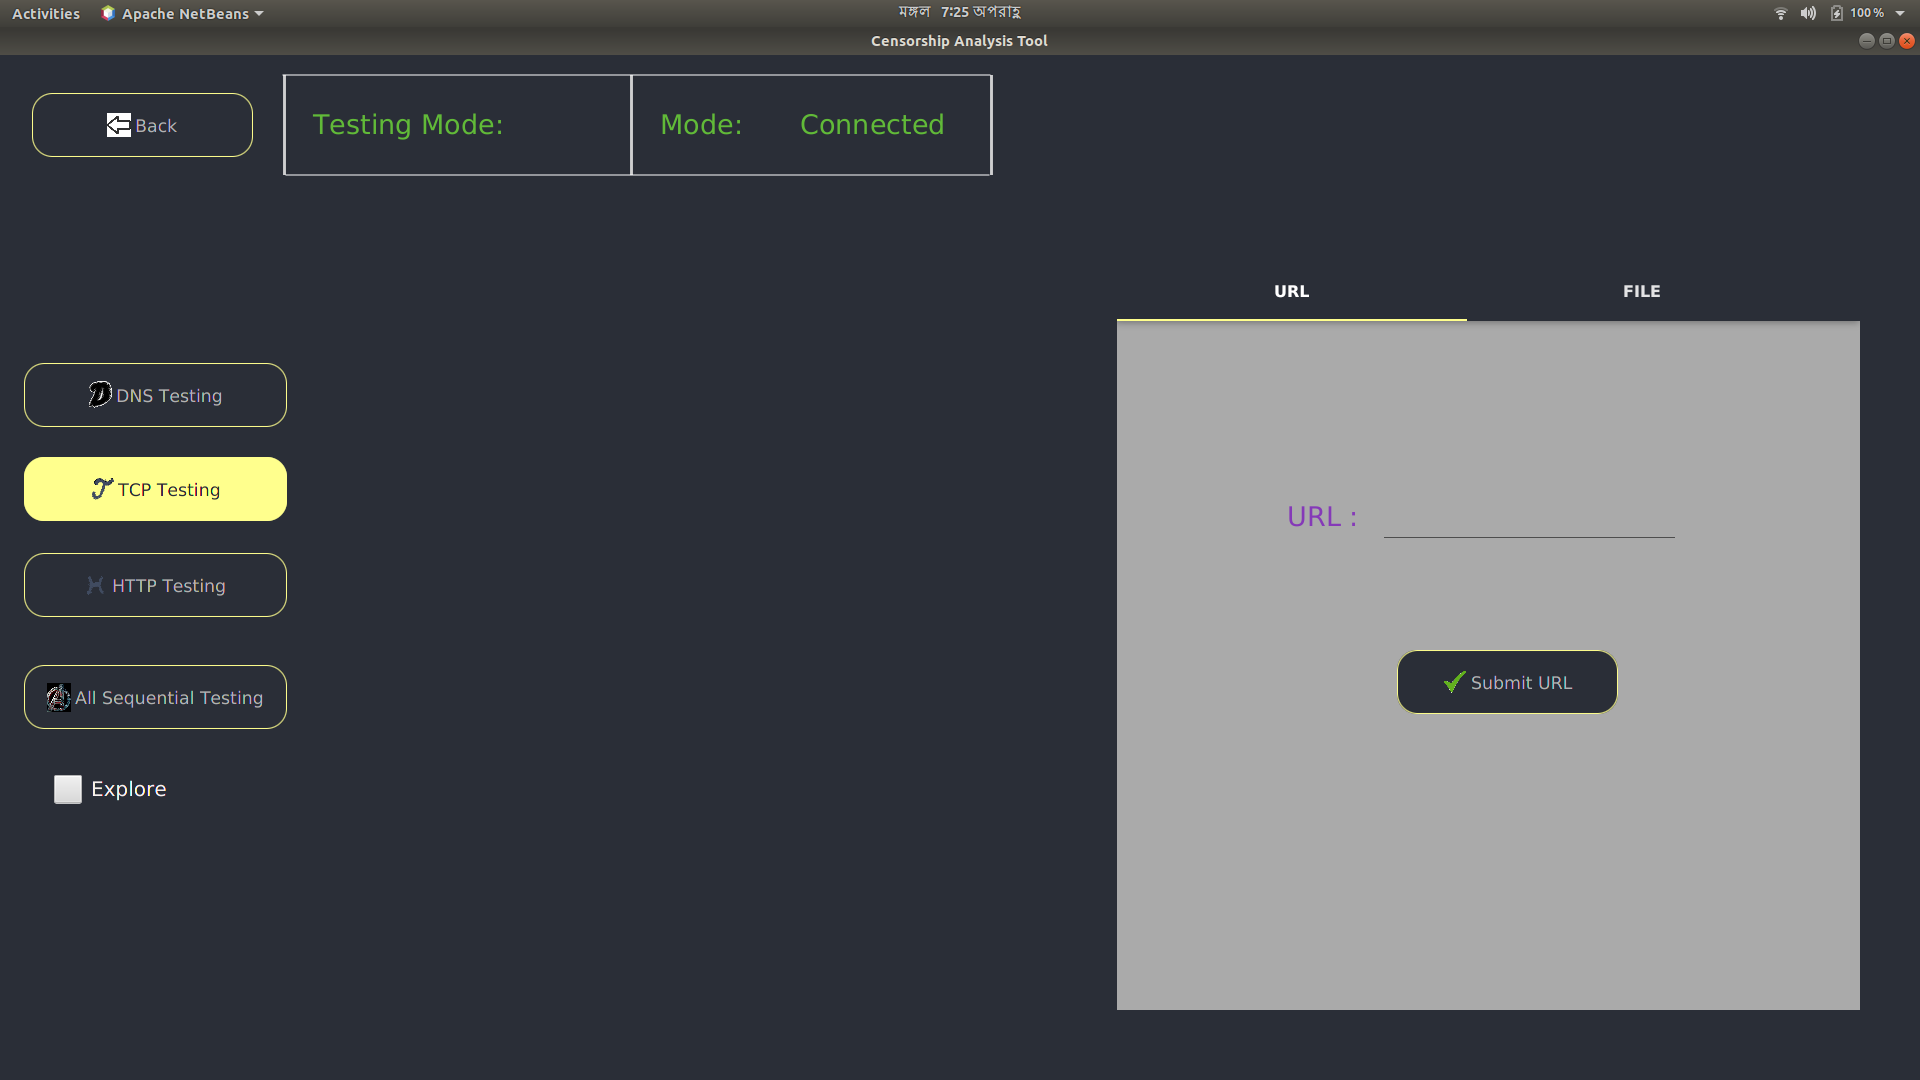
\includegraphics[width=\textwidth]{usersite/17tcptest.png}
    \caption{TCP Testing button is selected}
    \label{fig:user16}
\end{figure}

\begin{figure}[h]
    \centering
    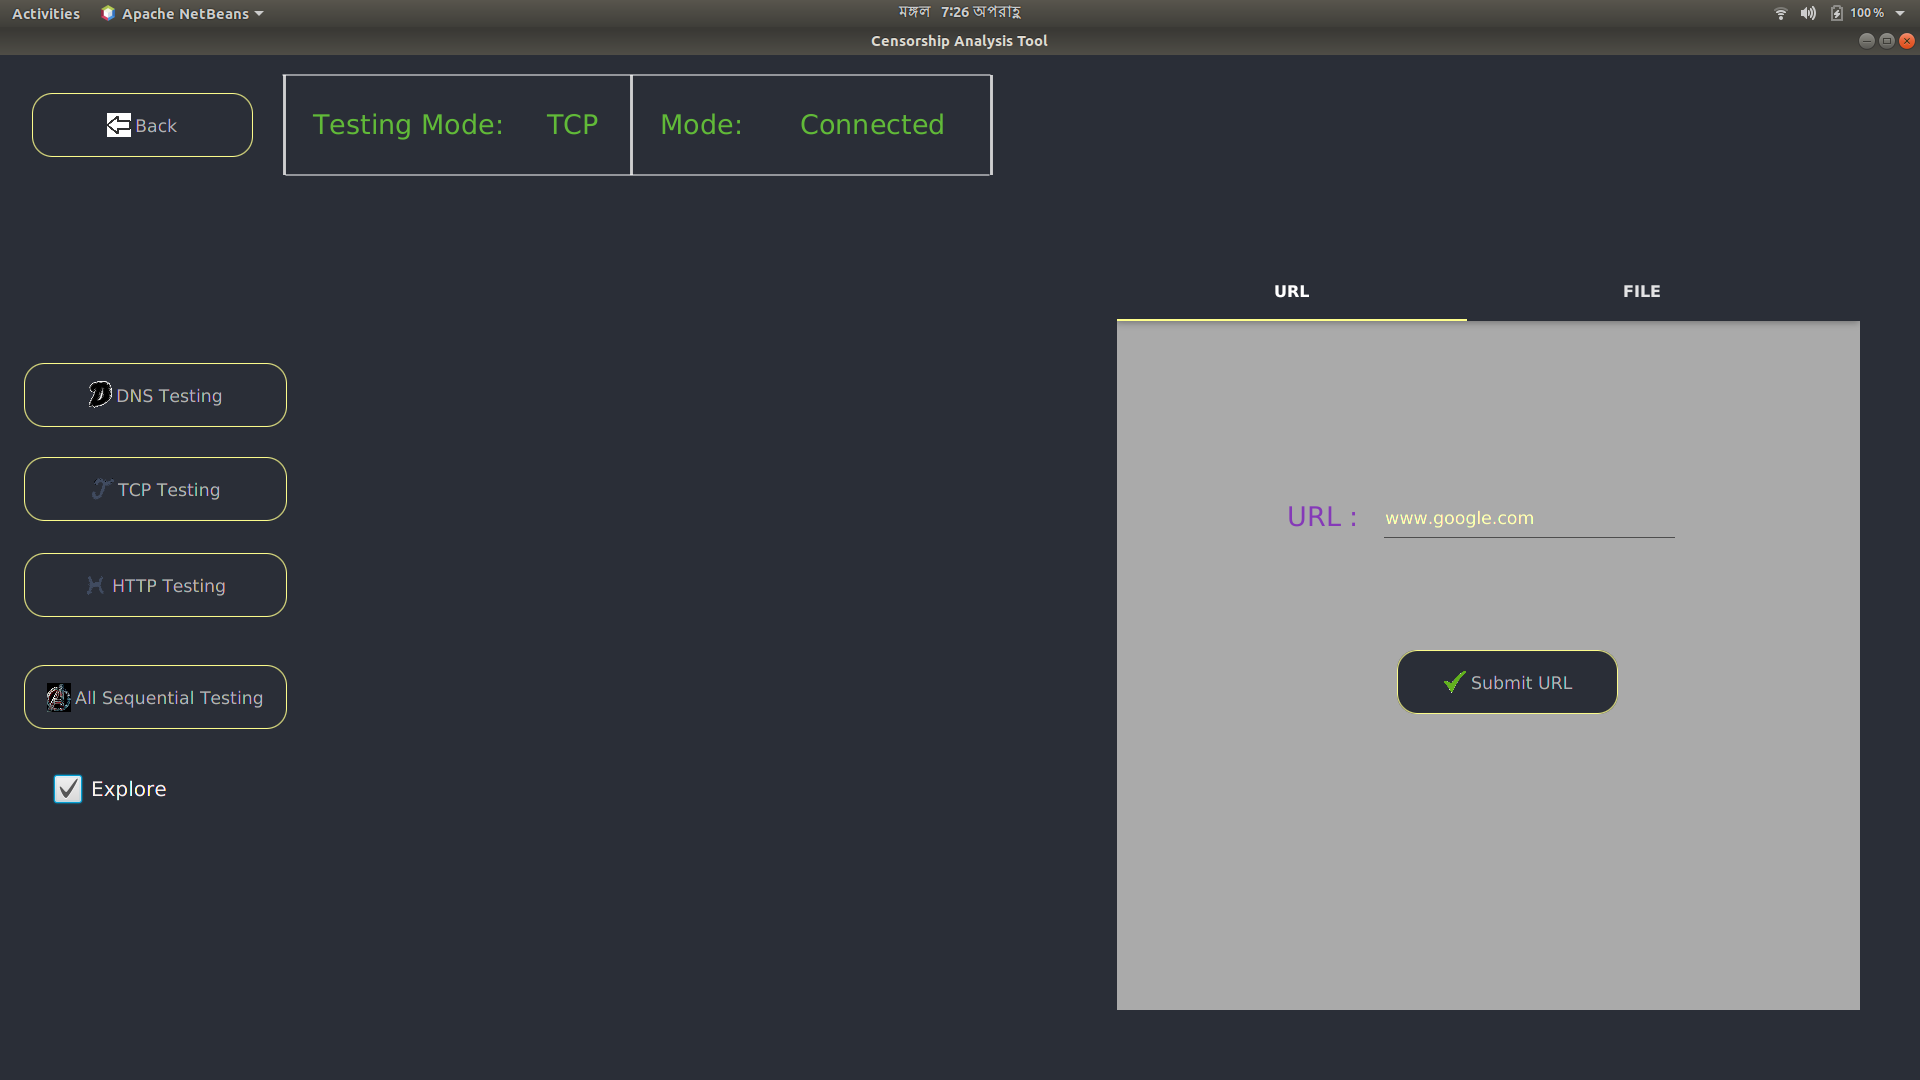
\includegraphics[width=\textwidth]{usersite/18tcptest2.png}
    \caption{TCP Testing input are given}
    \label{fig:user17}
\end{figure}

Real time underlying operation are given when a user click on \emph{Click for Details} button.

\begin{figure}[h]
    \centering
    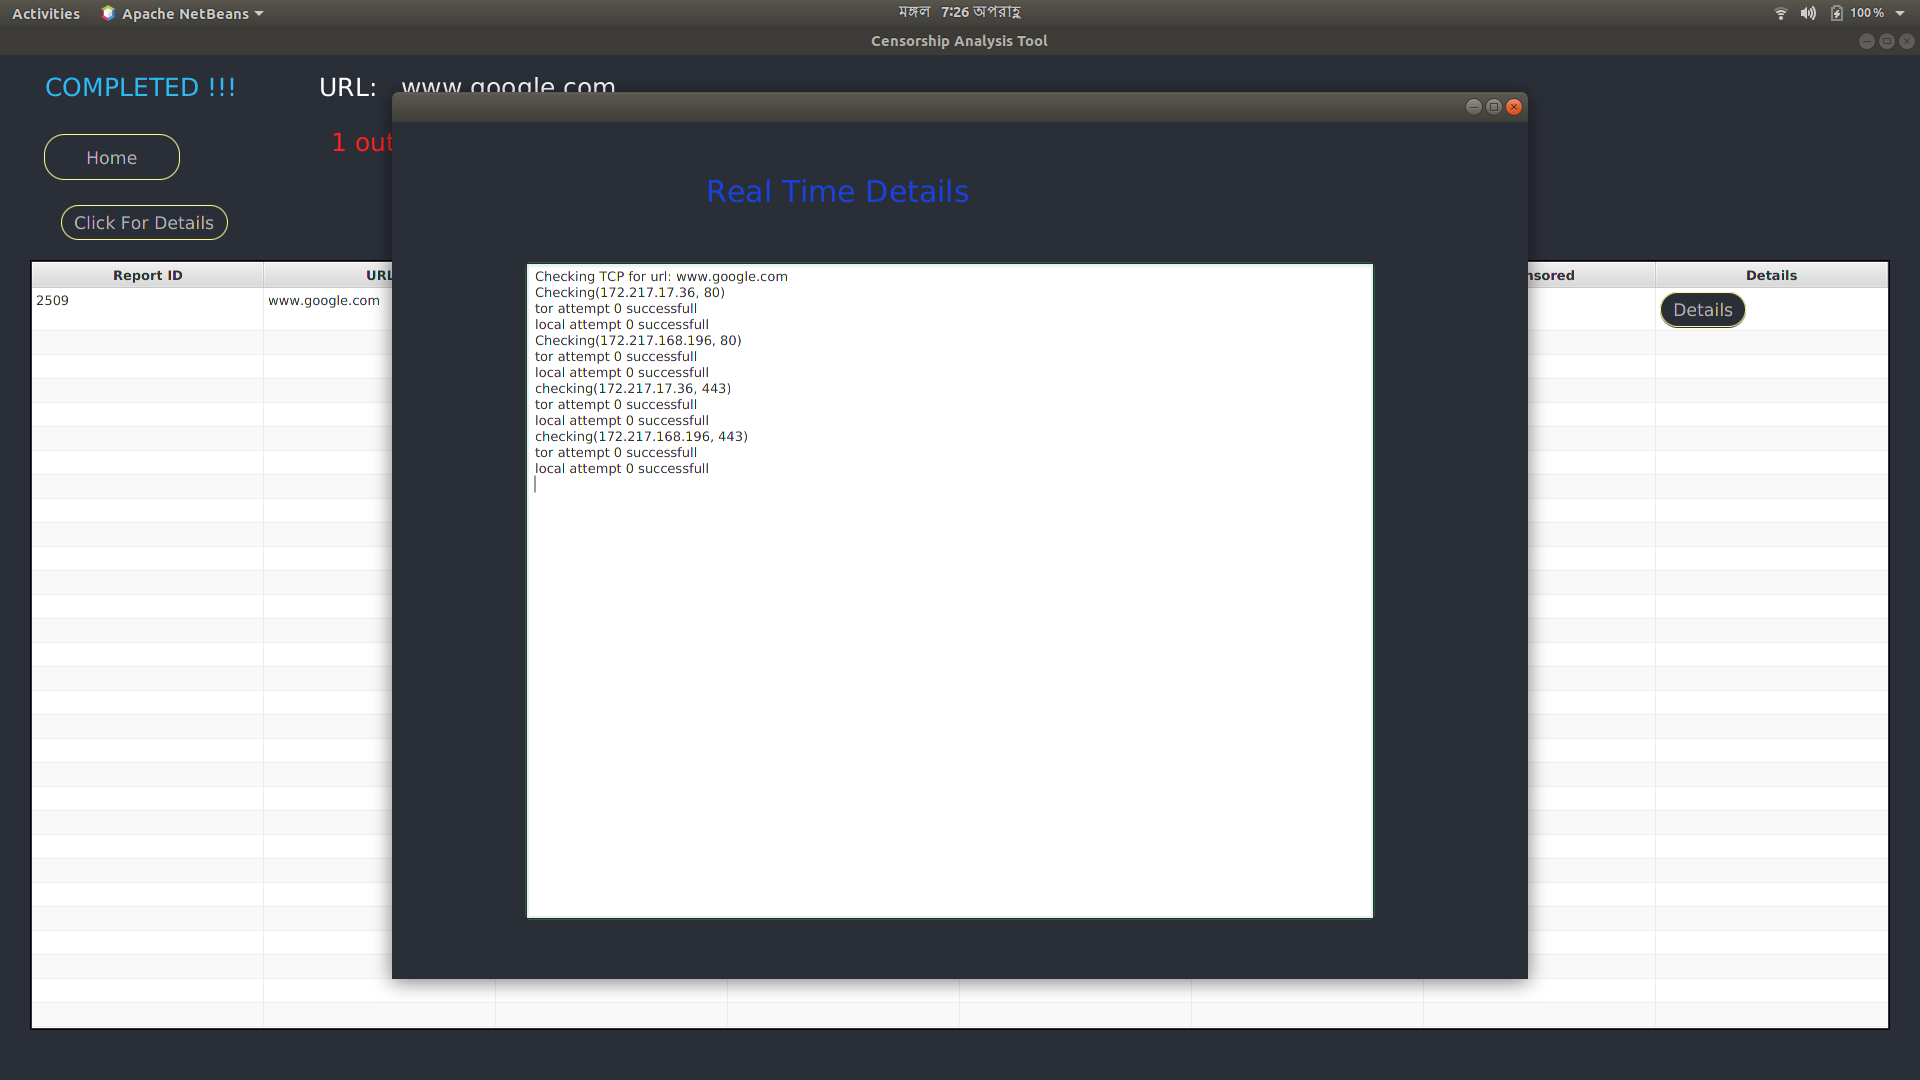
\includegraphics[width=\textwidth]{usersite/19realtime.png}
    \caption{After Click for Details button clicking real time data are shown }
    \label{fig:user18}
\end{figure}

\begin{figure}[h]
    \centering
    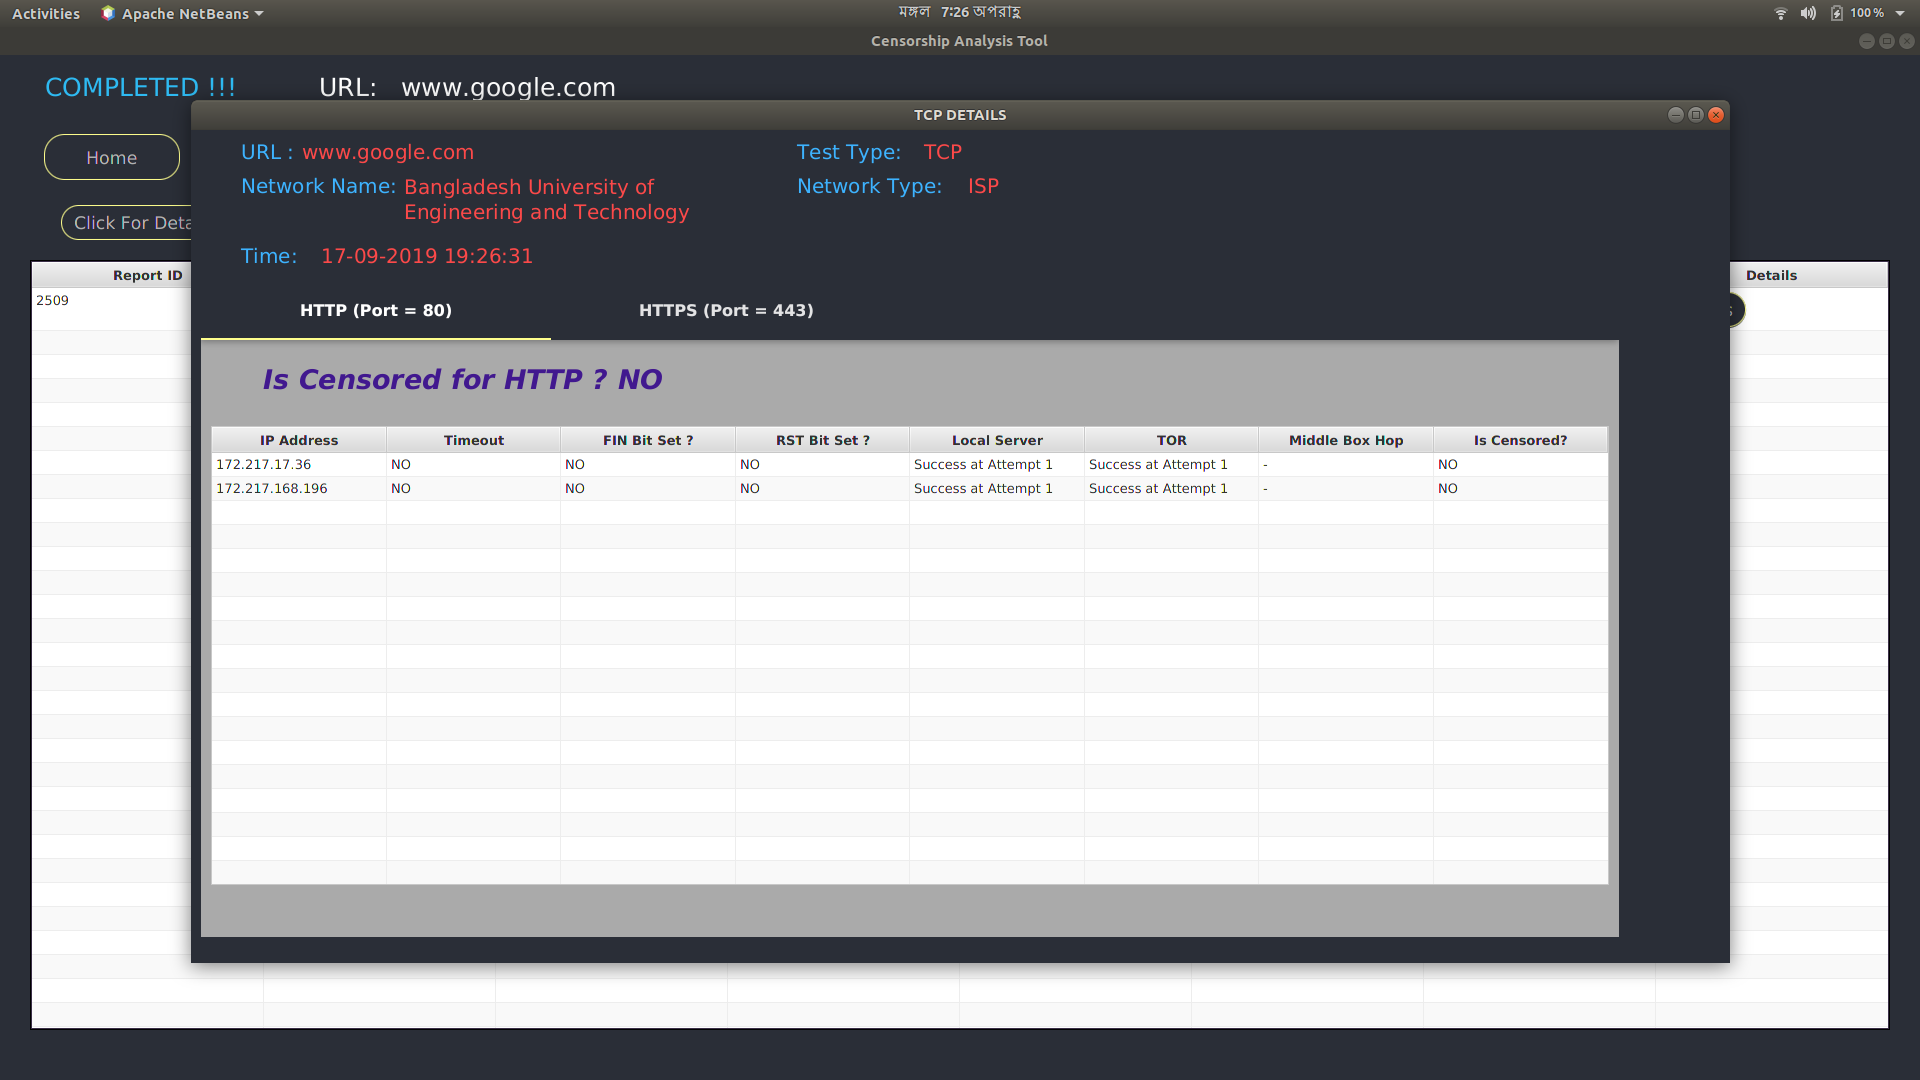
\includegraphics[width=\textwidth]{usersite/20tcpdetailshttp.png}
    \caption{HTTP port 80 details}
    \label{fig:user19}
\end{figure}

\begin{figure}[h]
    \centering
    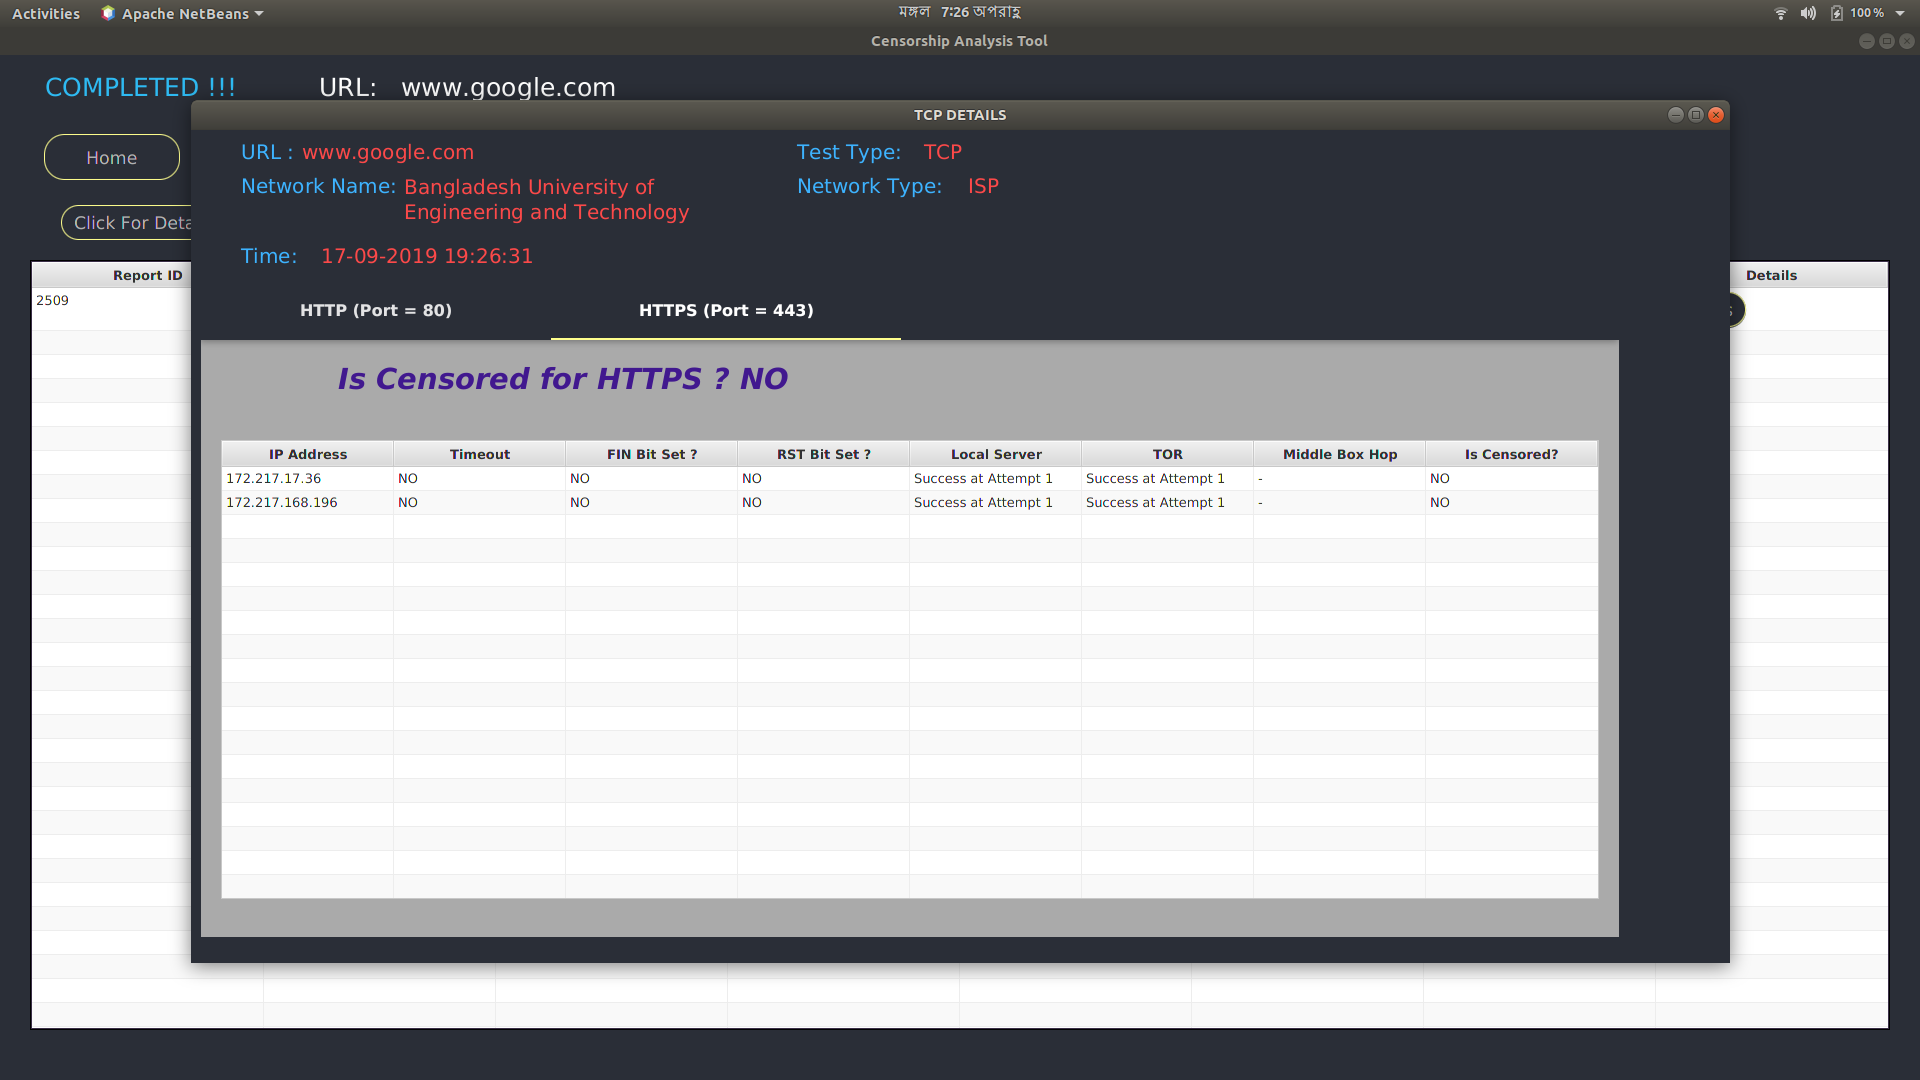
\includegraphics[width=\textwidth]{usersite/21tcpdetailshttps.png}
    \caption{HTTPS port 435 details}
    \label{fig:user20}
\end{figure}

\begin{figure}[h]
    \centering
    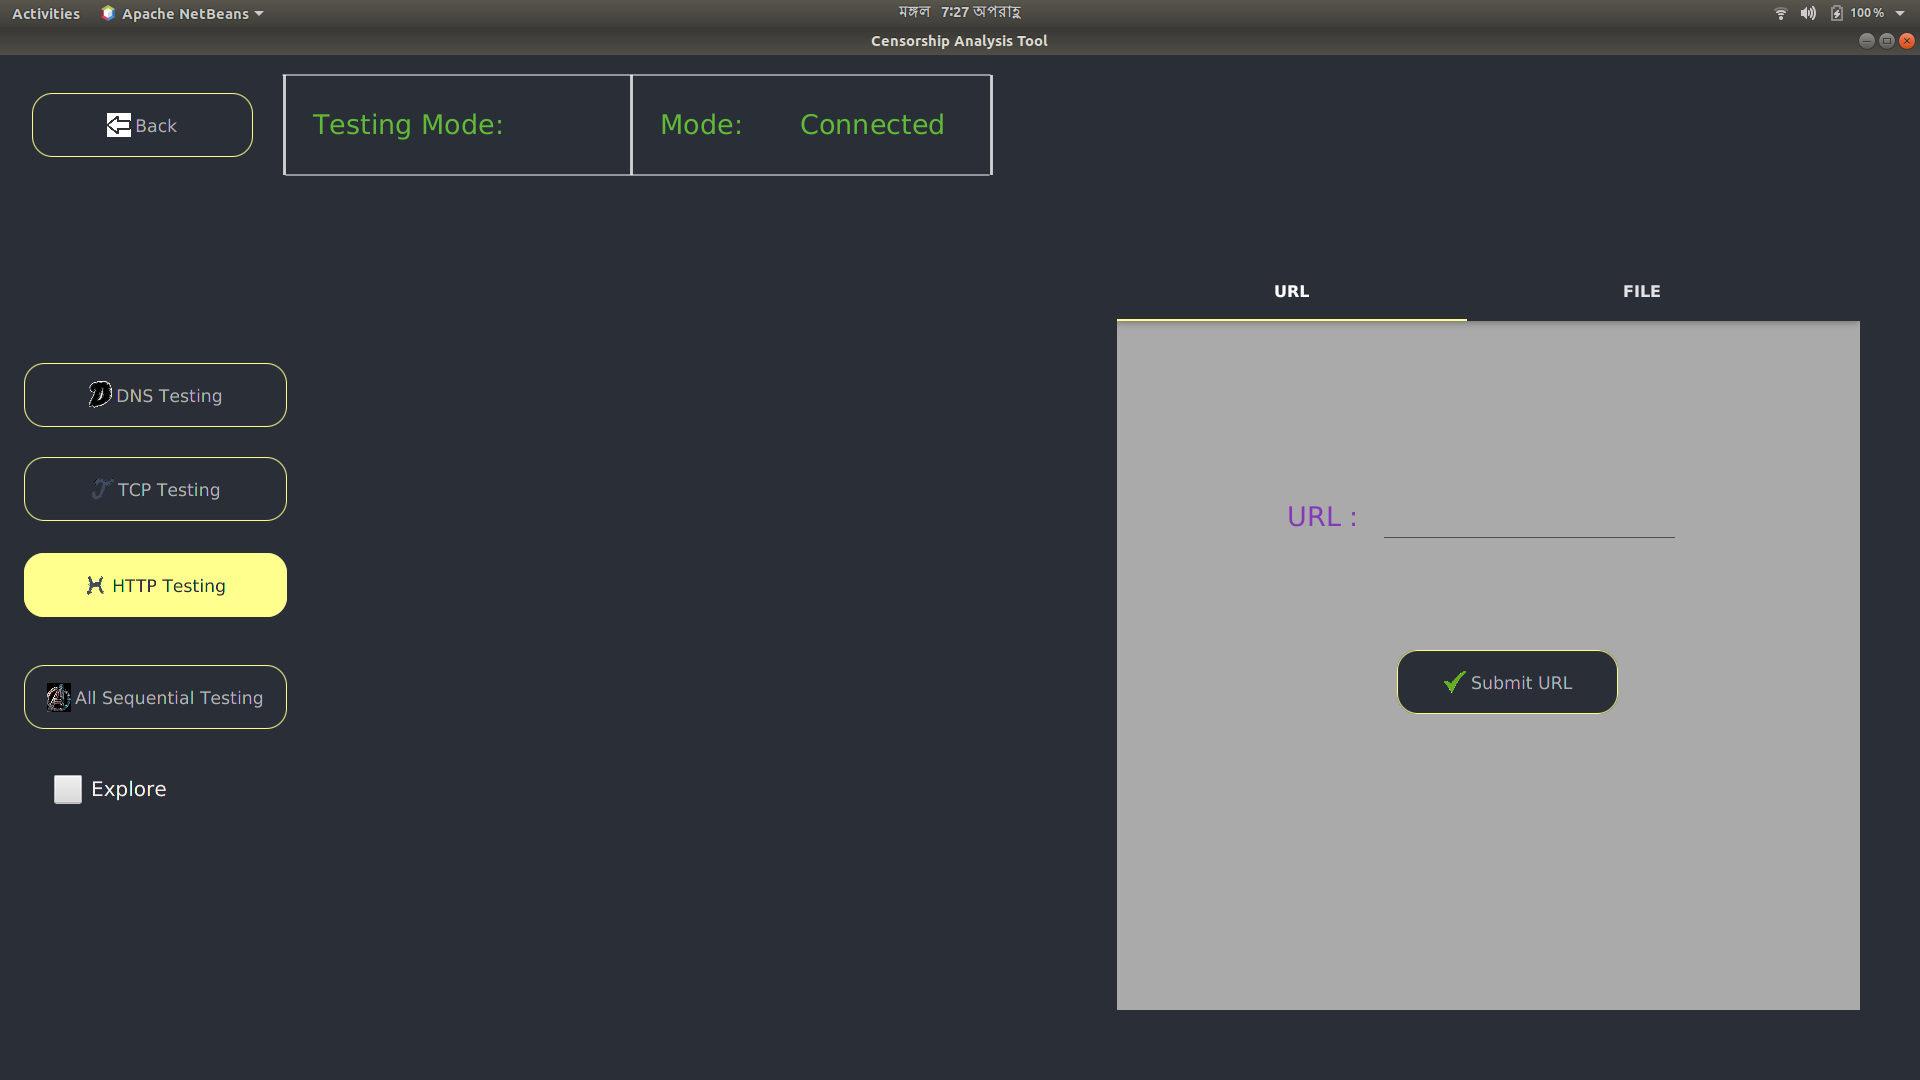
\includegraphics[width=\textwidth]{usersite/22httptest.png}
    \caption{HTTP Test button is clicked}
    \label{fig:user21}
\end{figure}

\begin{figure}[h]
    \centering
    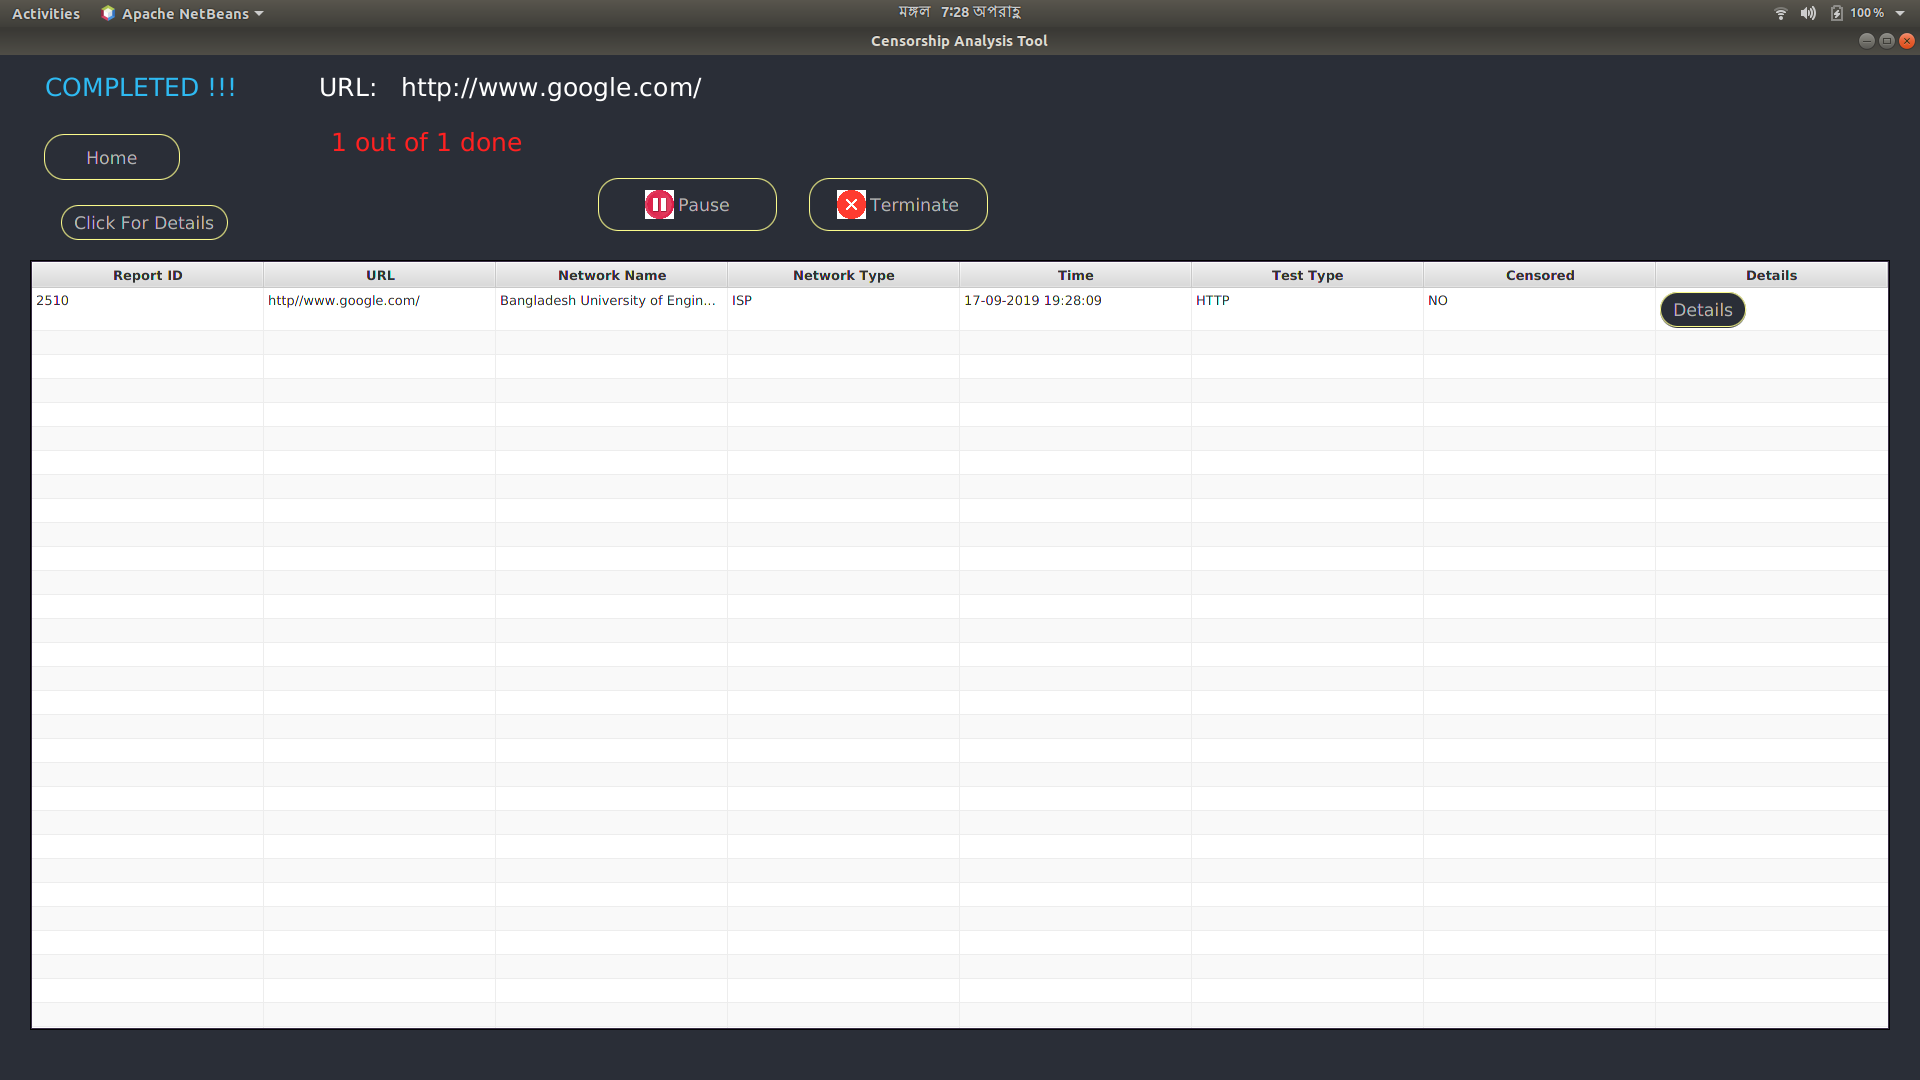
\includegraphics[width=\textwidth]{usersite/23httptestdone.png}
    \caption{HTTP Test done for 1 url}
    \label{fig:user22}
\end{figure}

\begin{figure}[h]
    \centering
    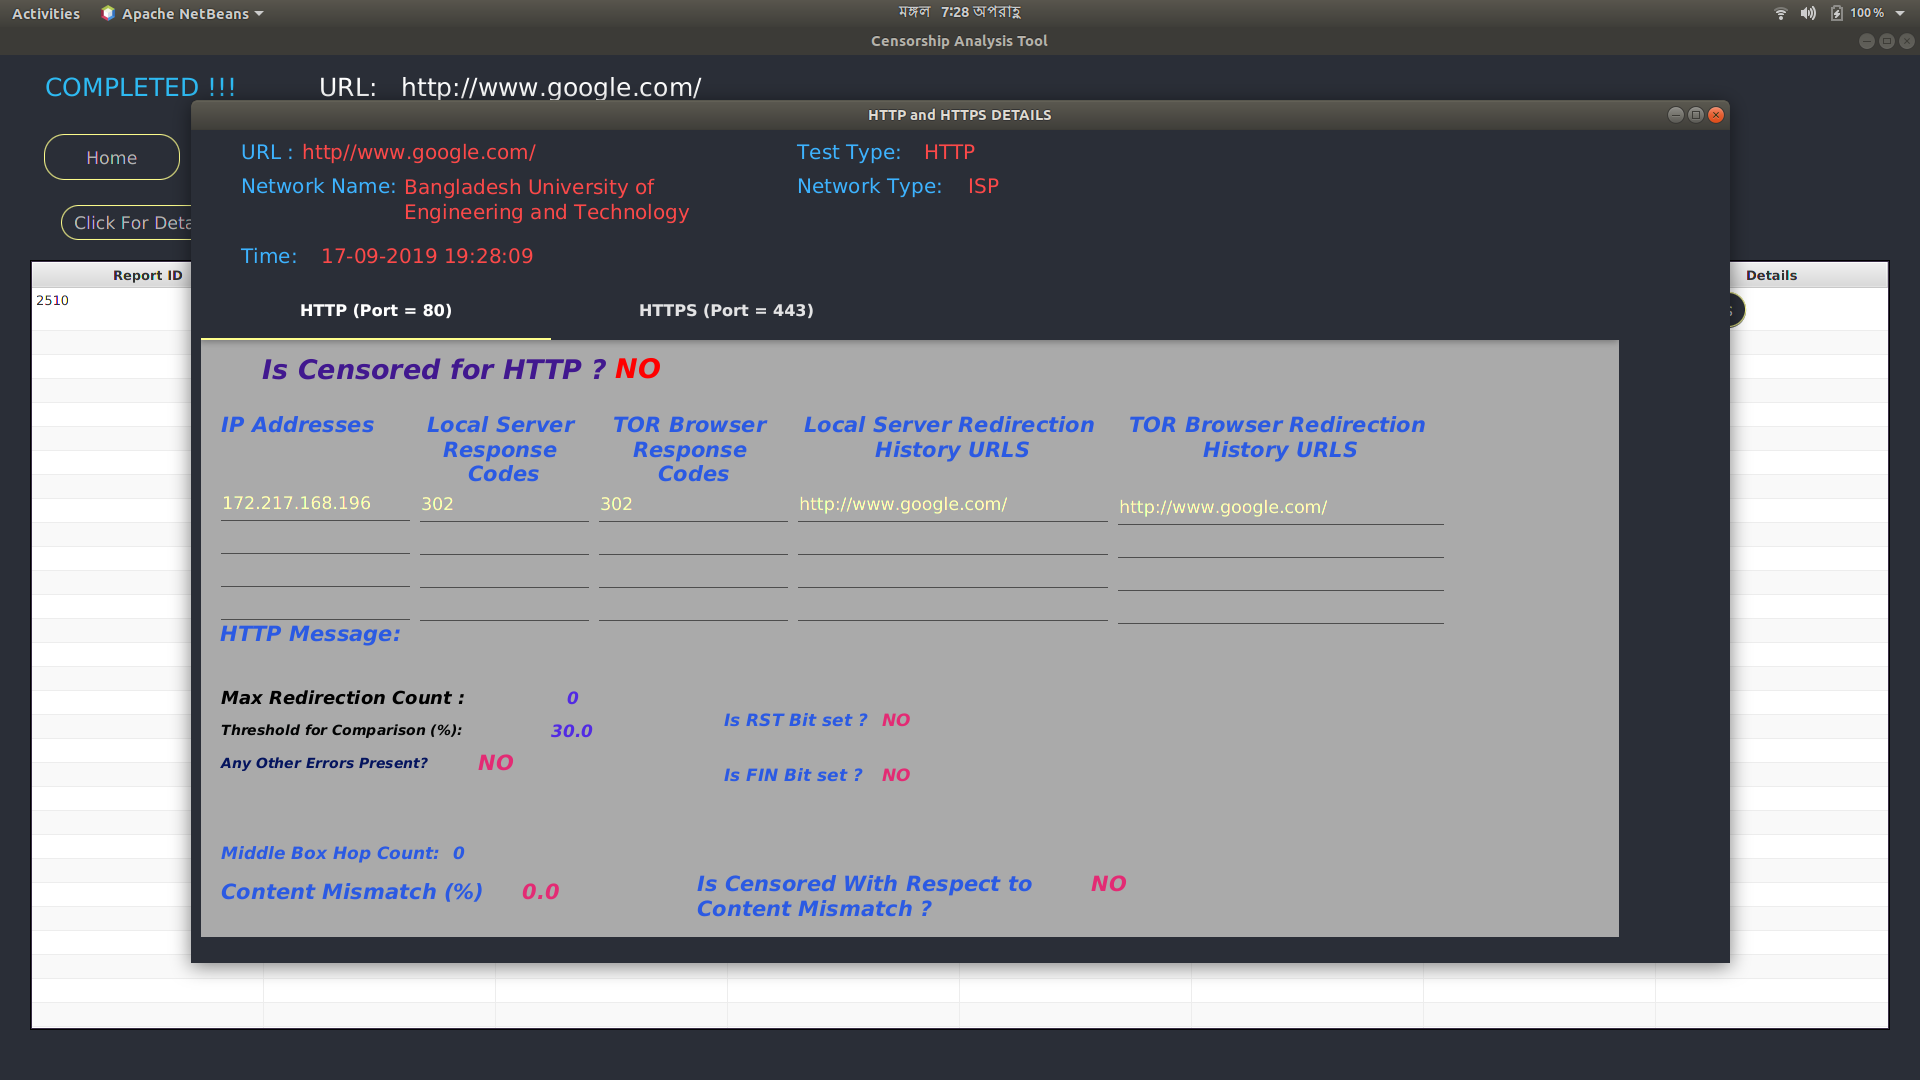
\includegraphics[width=\textwidth]{usersite/24httpdetails.png}
    \caption{HTTP port 80 details for HTTP test}
    \label{fig:user23}
\end{figure}

\begin{figure}[h]
    \centering
    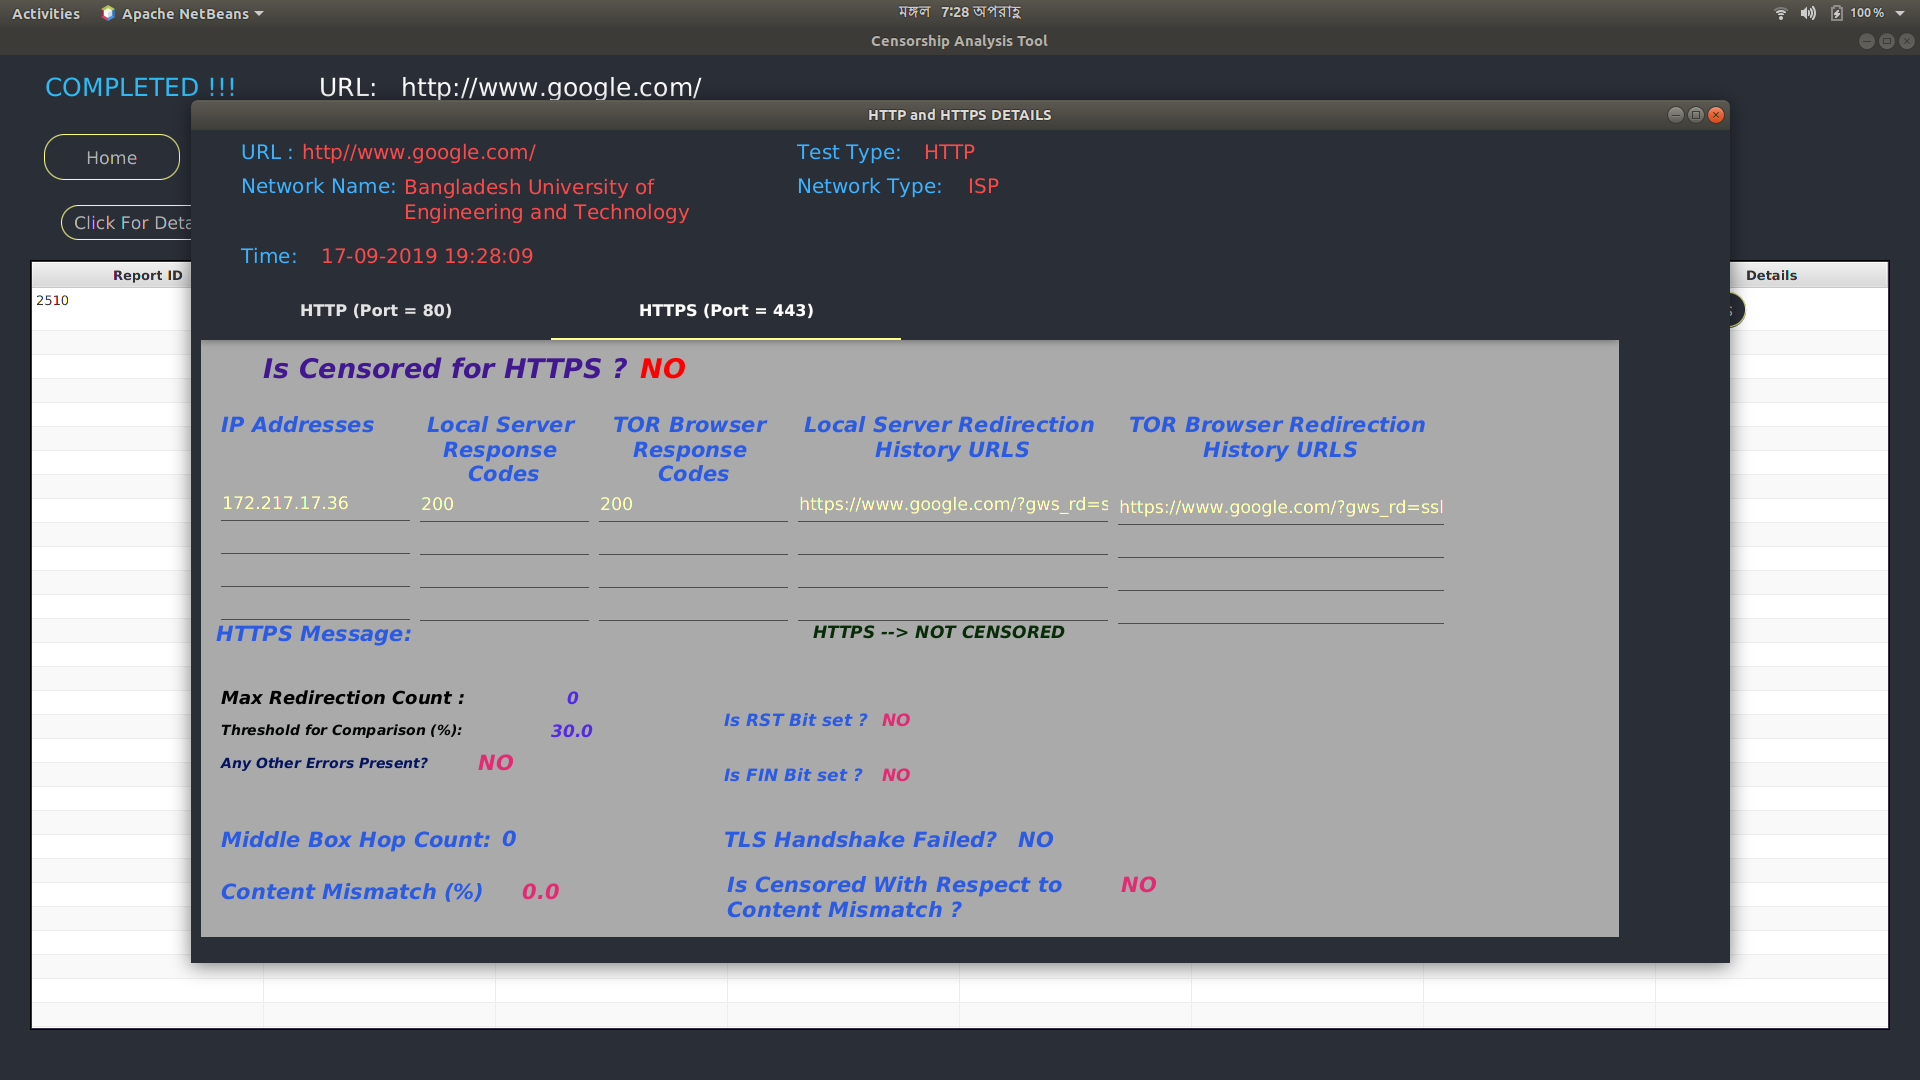
\includegraphics[width=\textwidth]{usersite/25httpsdetails.png}
    \caption{HTTPS port 435 details for HTTP test}
    \label{fig:user24}
\end{figure}

\begin{figure}[h]
    \centering
    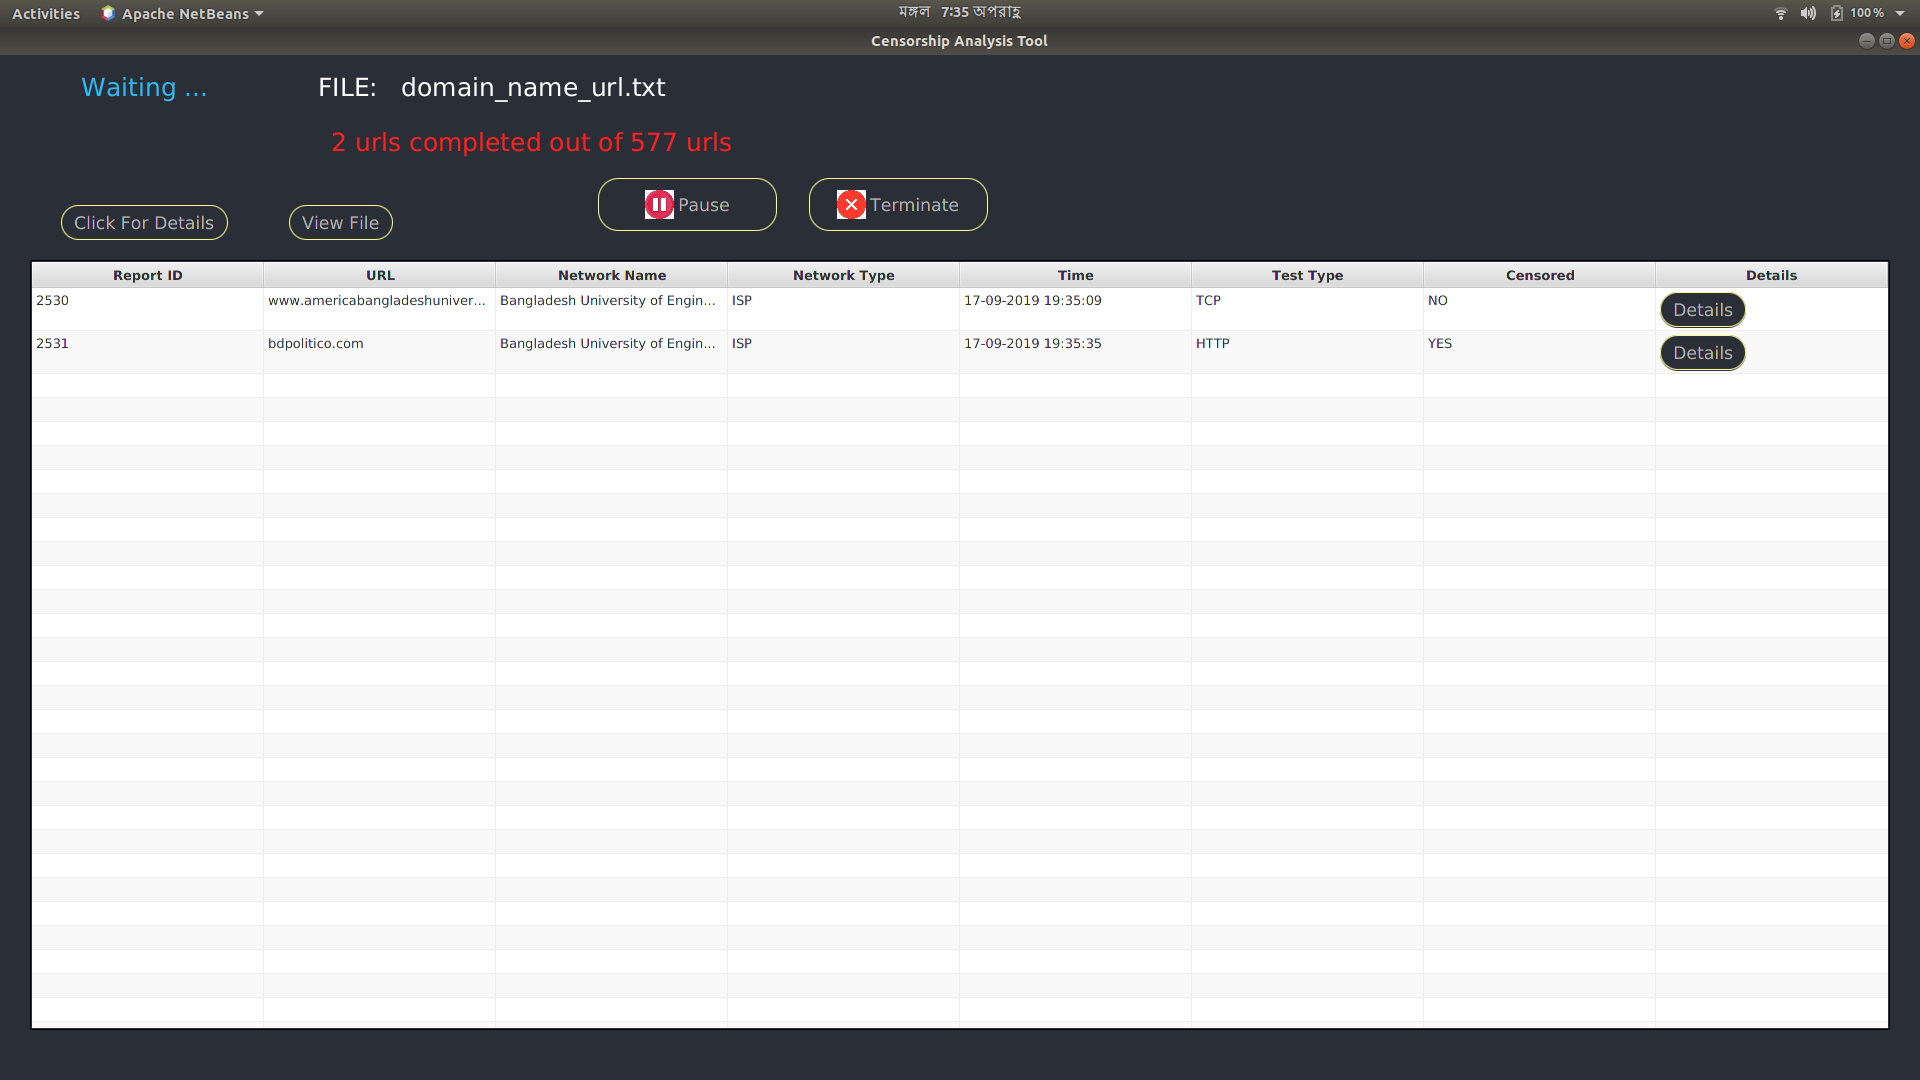
\includegraphics[width=\textwidth]{usersite/29filerunnin.png}
    \caption{A testing of file with urls started}
    \label{fig:user28}
\end{figure}


\begin{figure}[h]
    \centering
    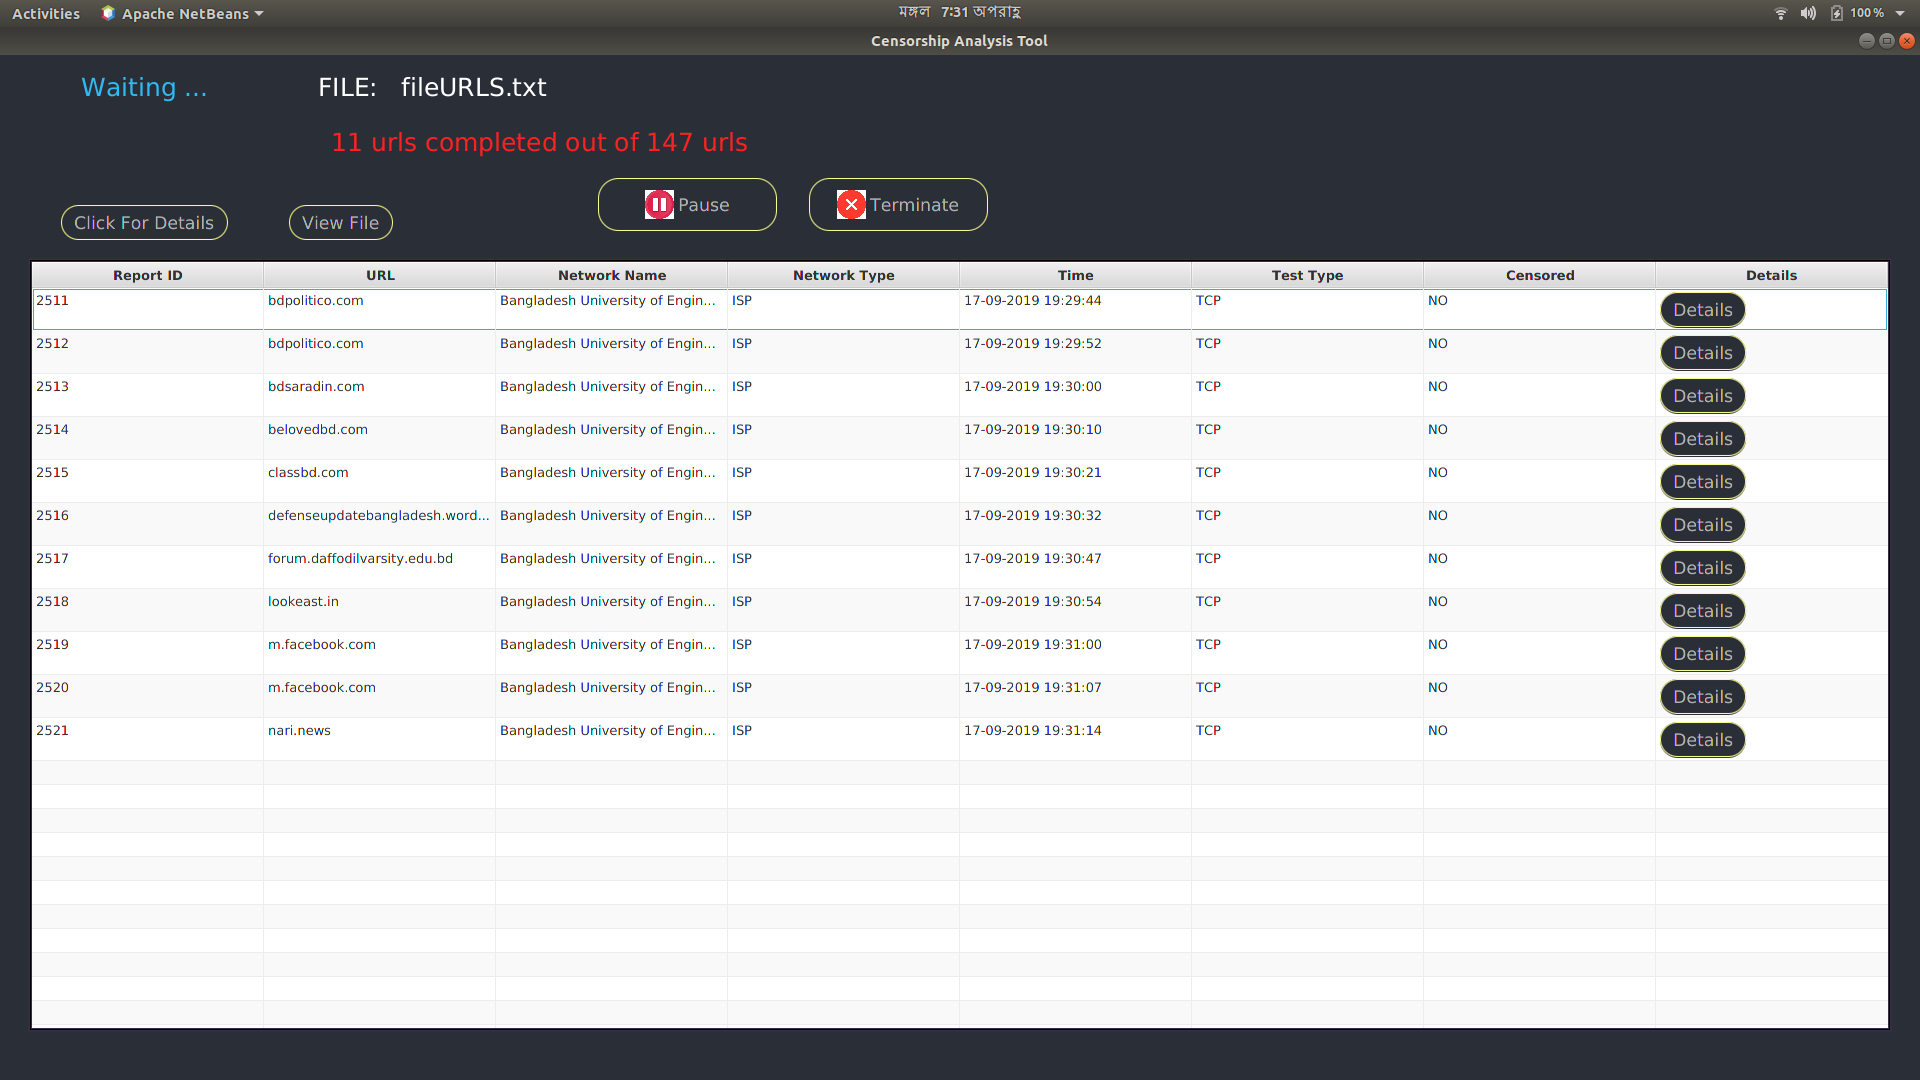
\includegraphics[width=\textwidth]{usersite/29filerunning.png}
    \caption{The testing of file with urls is going on}
    \label{fig:user29}
\end{figure}

\begin{figure}[h]
    \centering
    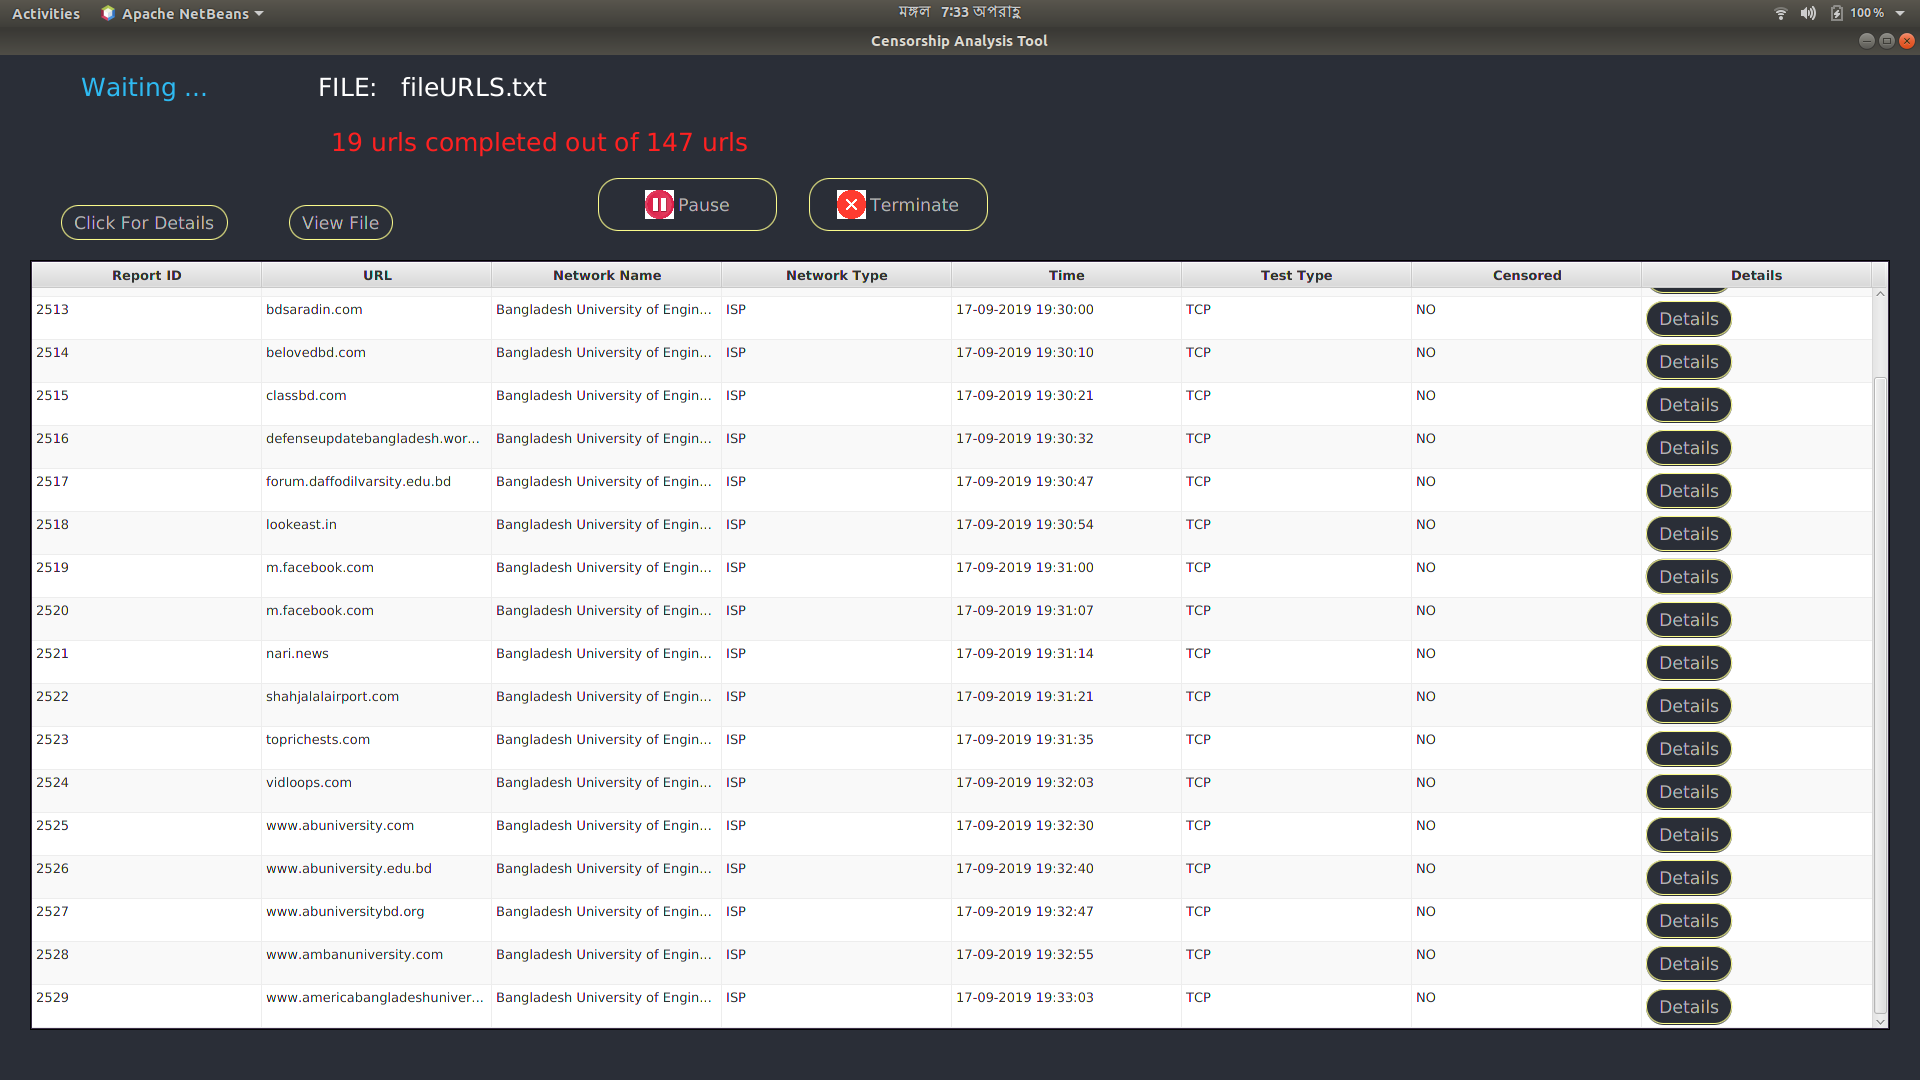
\includegraphics[width=\textwidth]{usersite/30filewaiting.png}
    \caption{The testing is going on}
    \label{fig:user30}
\end{figure}

\begin{figure}[h]
    \centering
    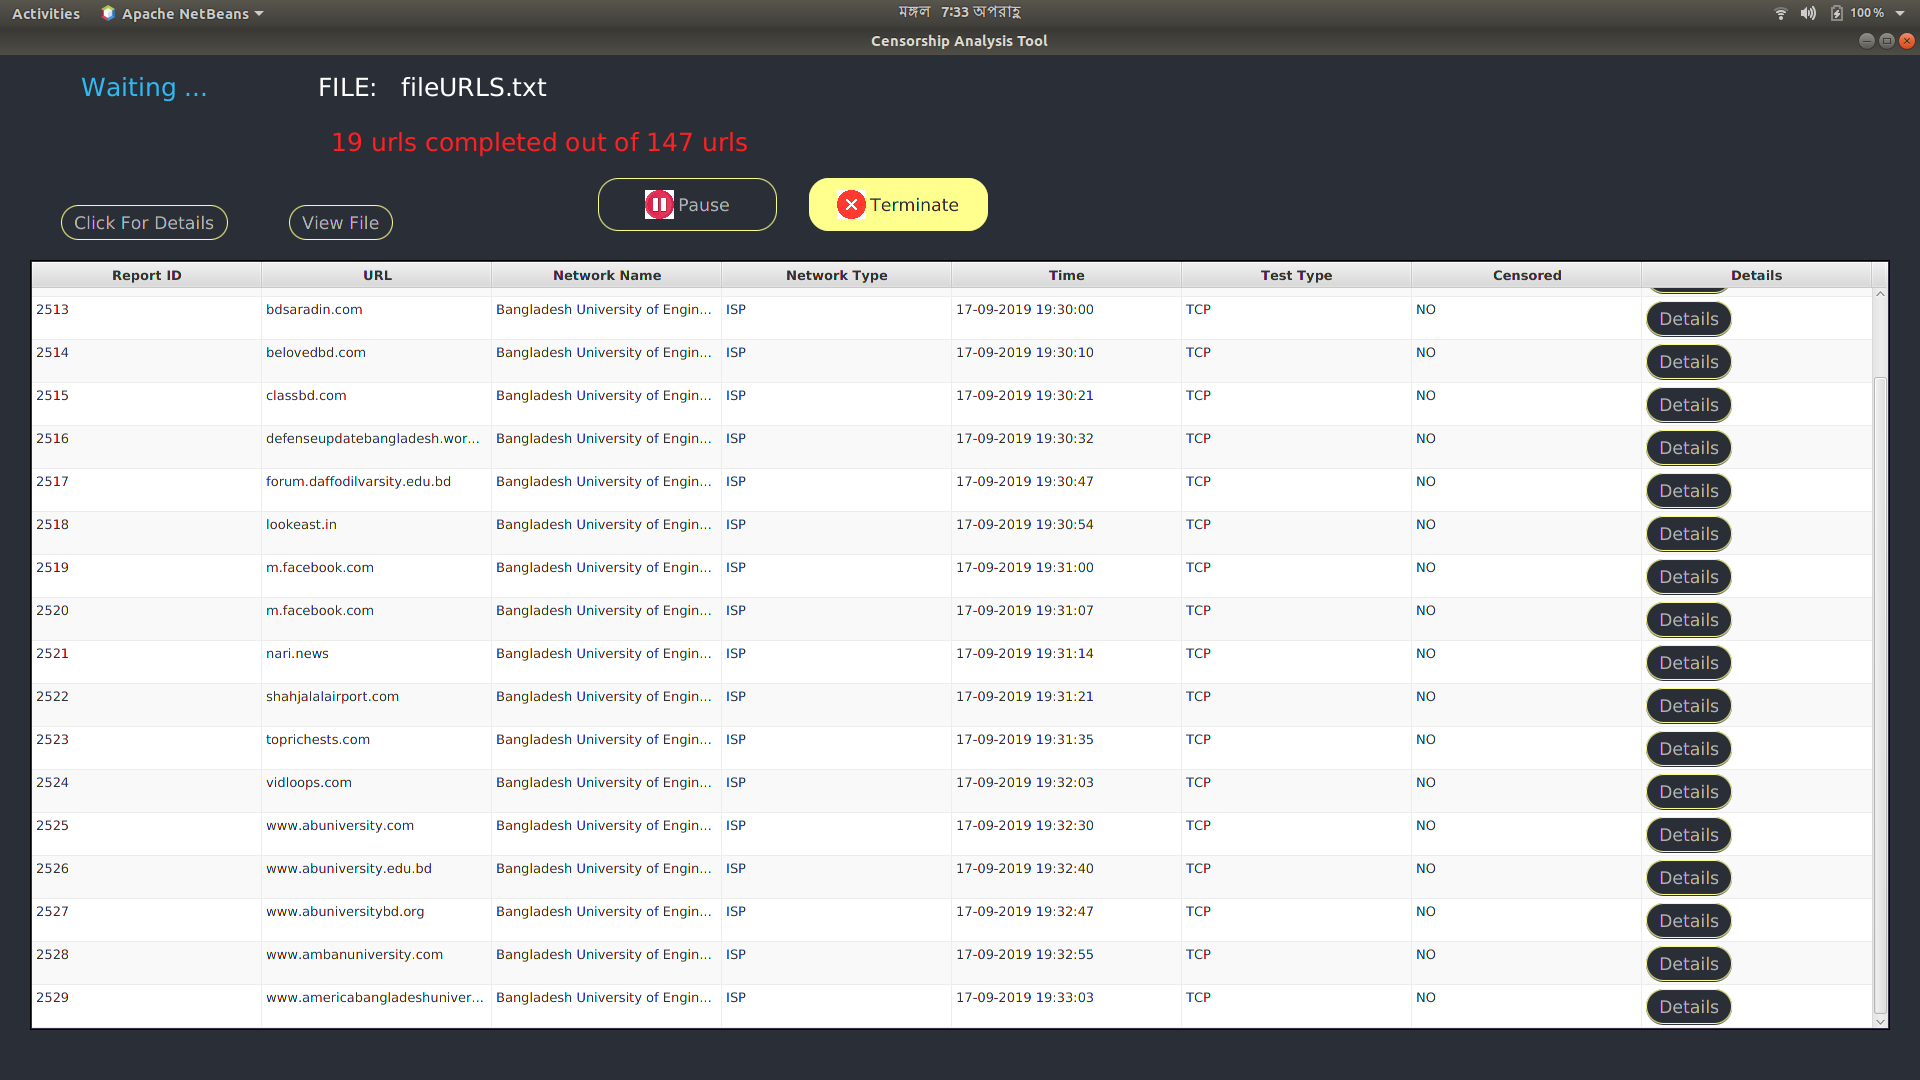
\includegraphics[width=\textwidth]{usersite/31filewaiting2.png}
    \caption{Terminating the test}
    \label{fig:user31}
\end{figure}

\begin{figure}[h]
    \centering
    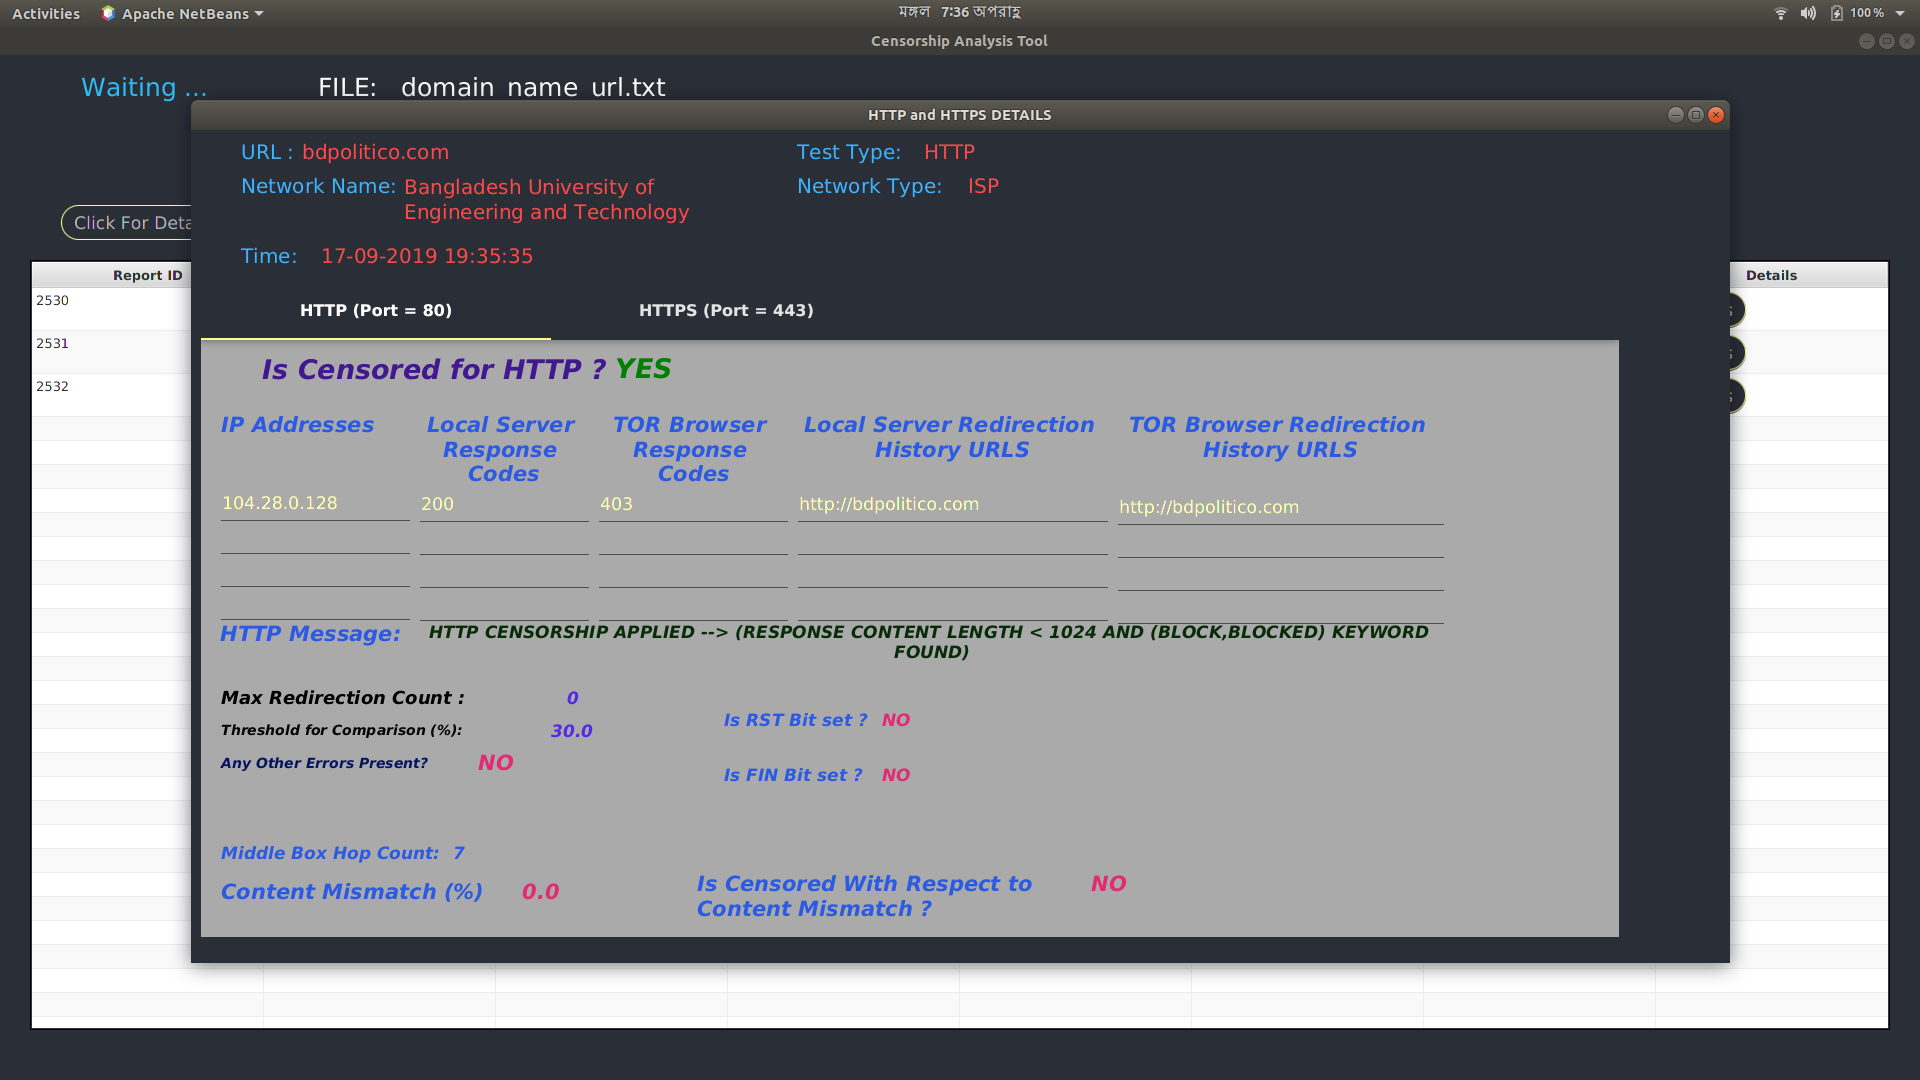
\includegraphics[width=\textwidth]{usersite/32httpdetails.png}
    \caption{HTTP port 80 data are seen}
    \label{fig:user32}
\end{figure}



\begin{figure}[h]
    \centering
    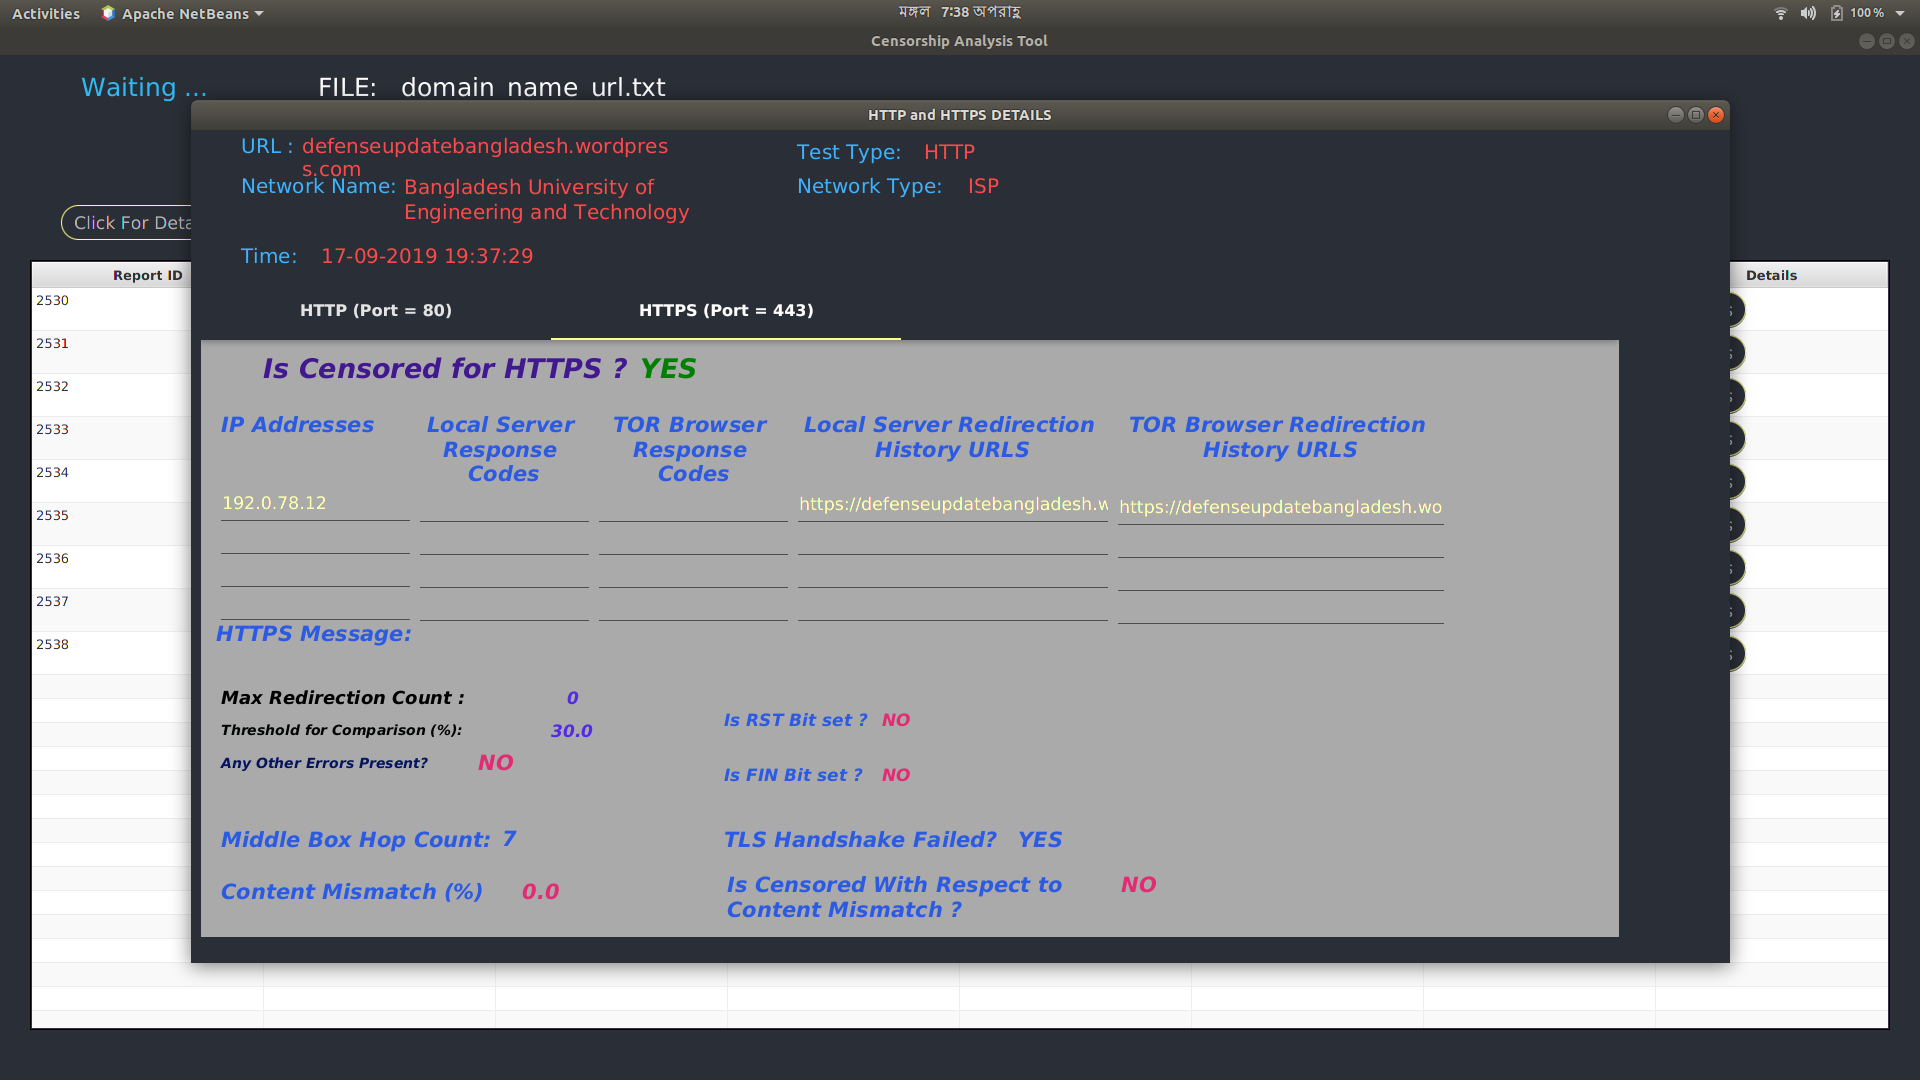
\includegraphics[width=\textwidth]{usersite/34httpsrealtime.png}
    \caption{HTTPS port 435 data are seen}
    \label{fig:user34}
\end{figure}

\begin{figure}[h]
    \centering
    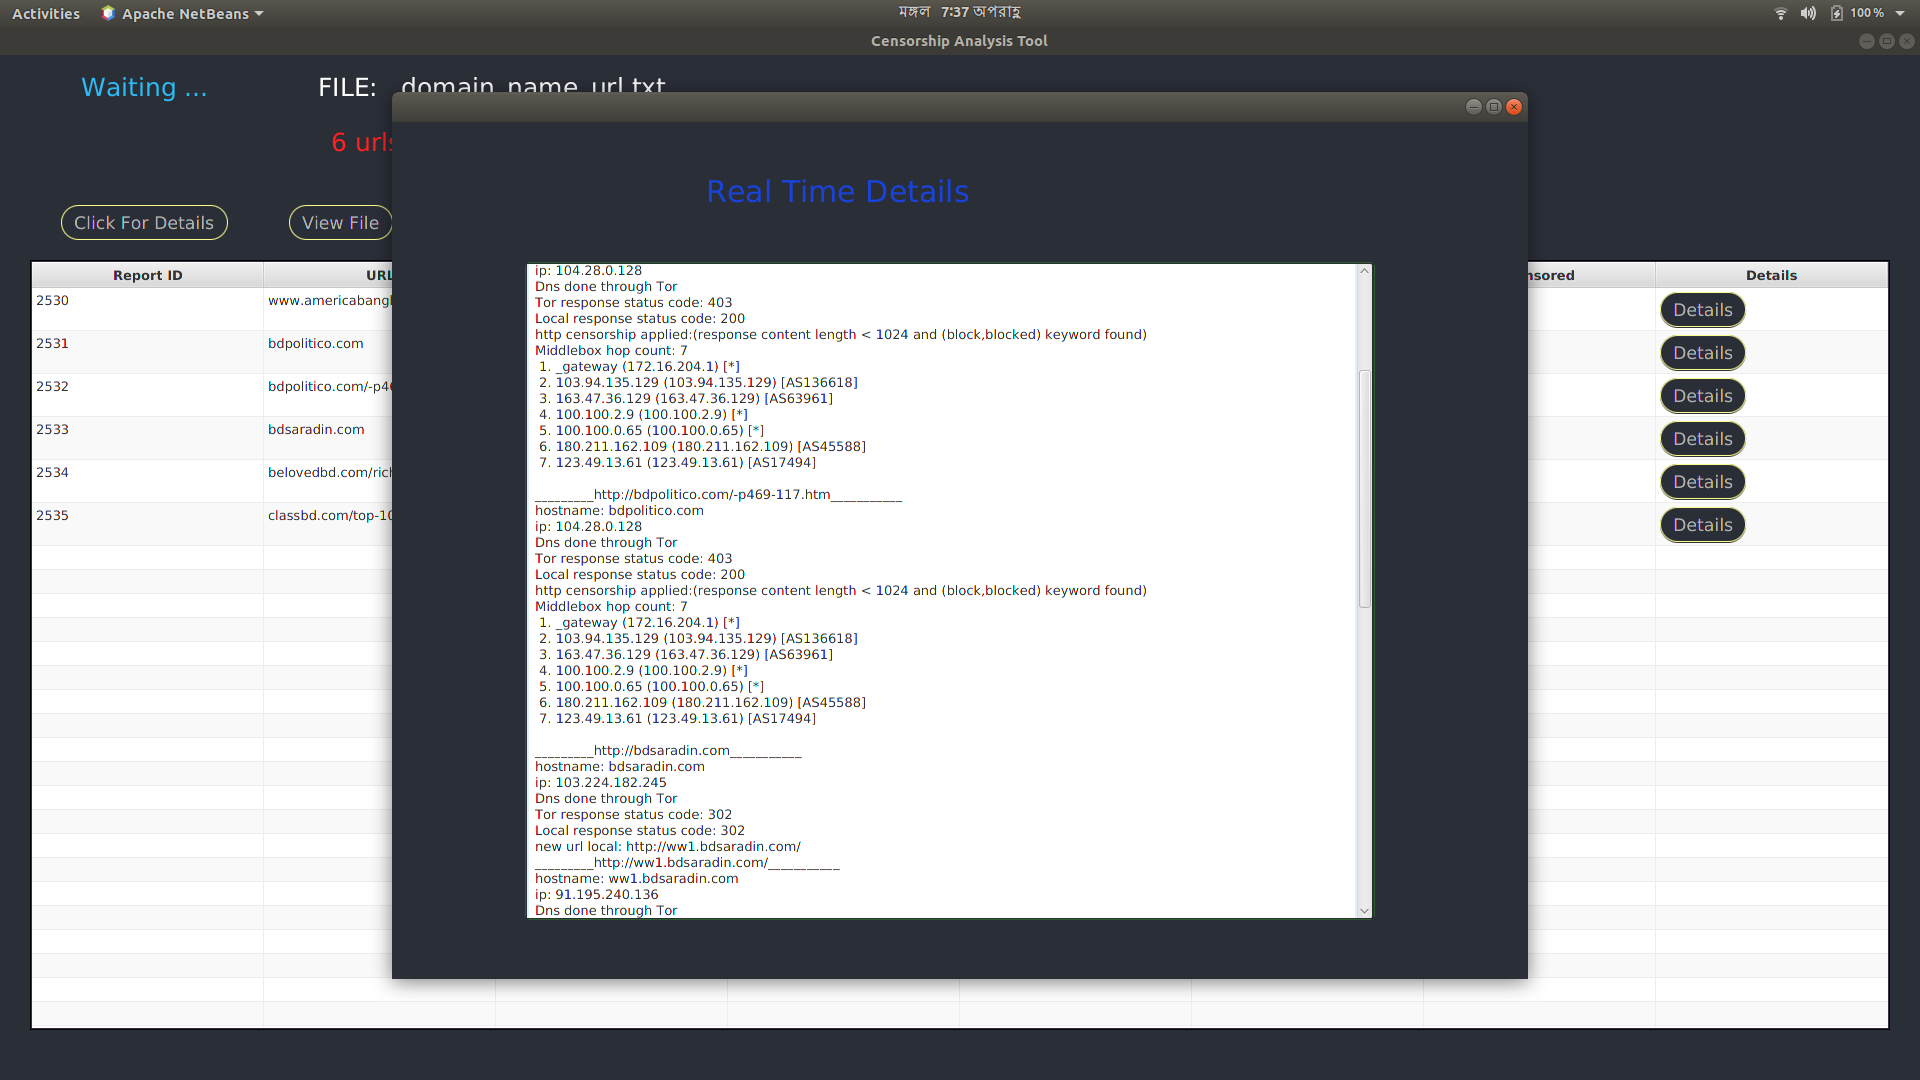
\includegraphics[width=\textwidth]{usersite/33httprealtime.png}
    \caption{HTTP real time operations}
    \label{fig:user33}
\end{figure}

\begin{figure}[h]
    \centering
    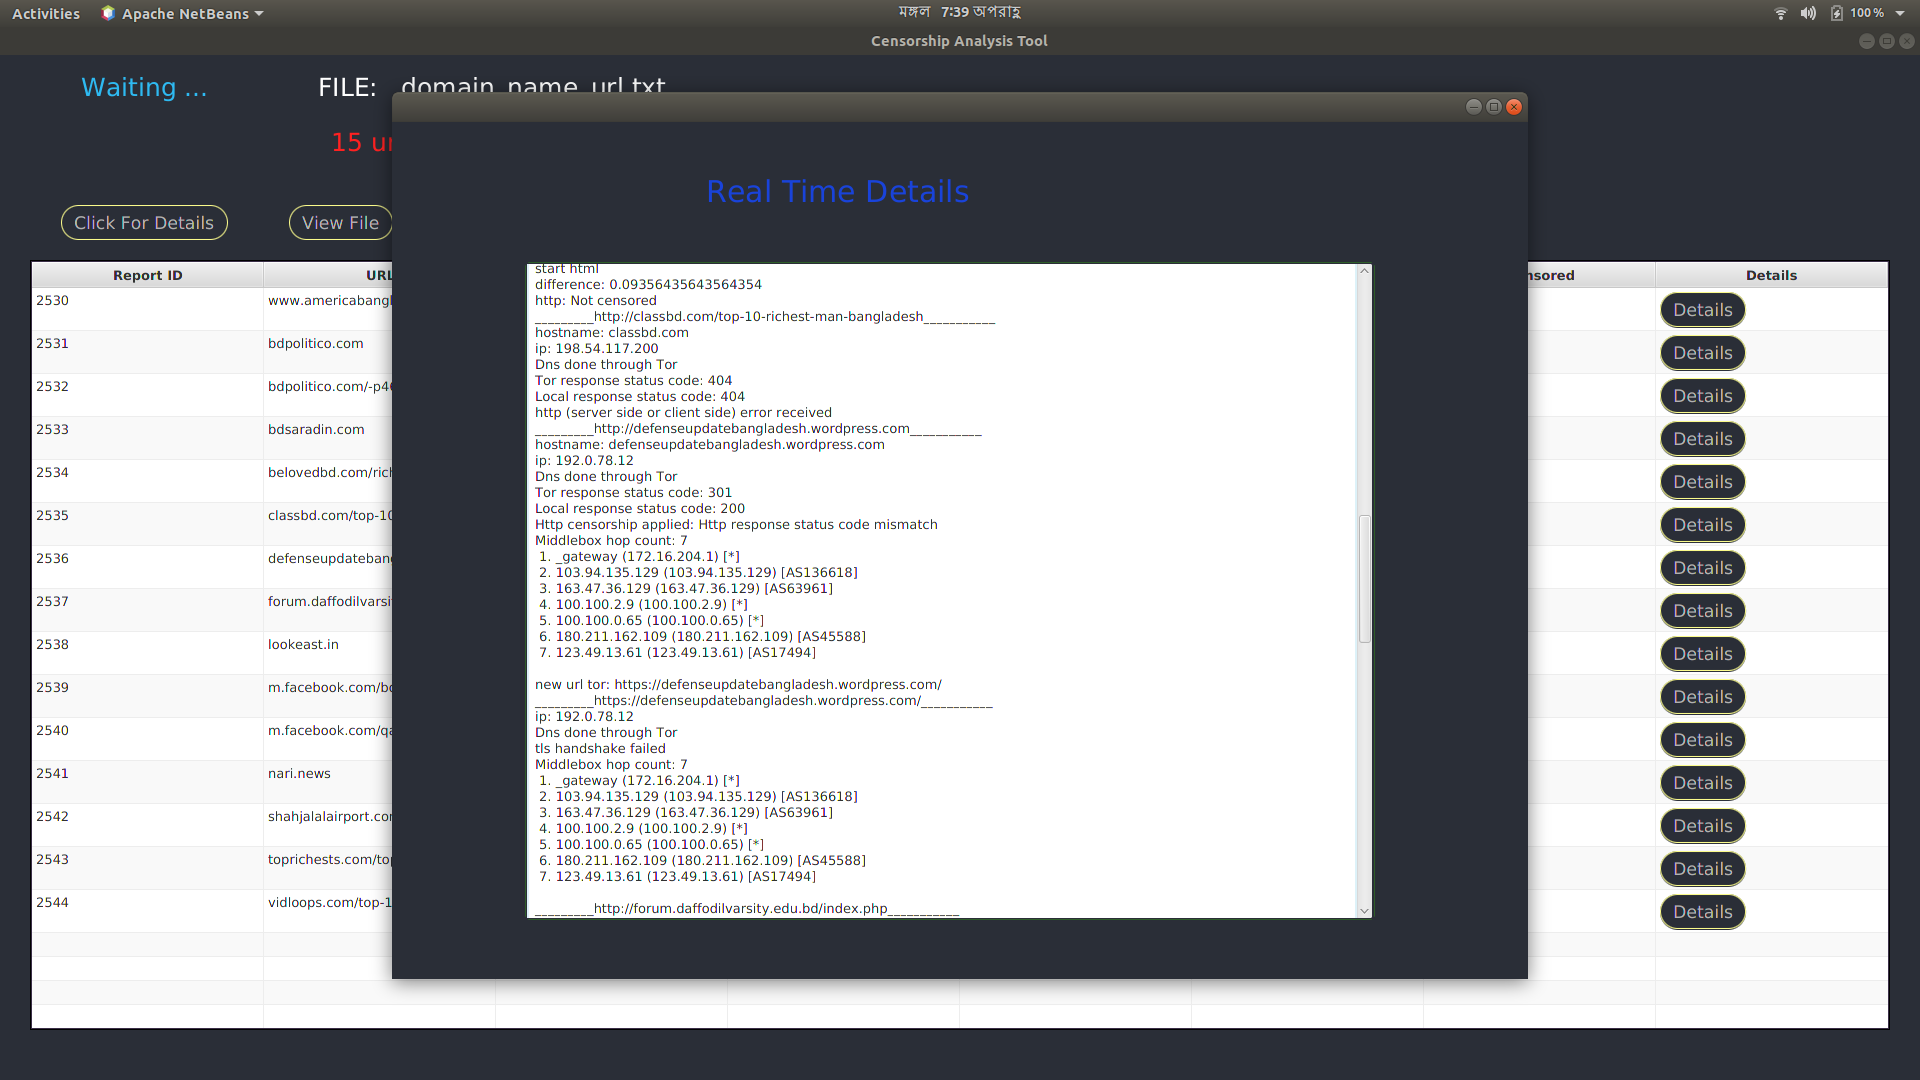
\includegraphics[width=\textwidth]{usersite/35realtimedetails.png}
    \caption{HTTP real time operations are going on}
    \label{fig:user35}
\end{figure}

\begin{figure}[h]
    \centering
    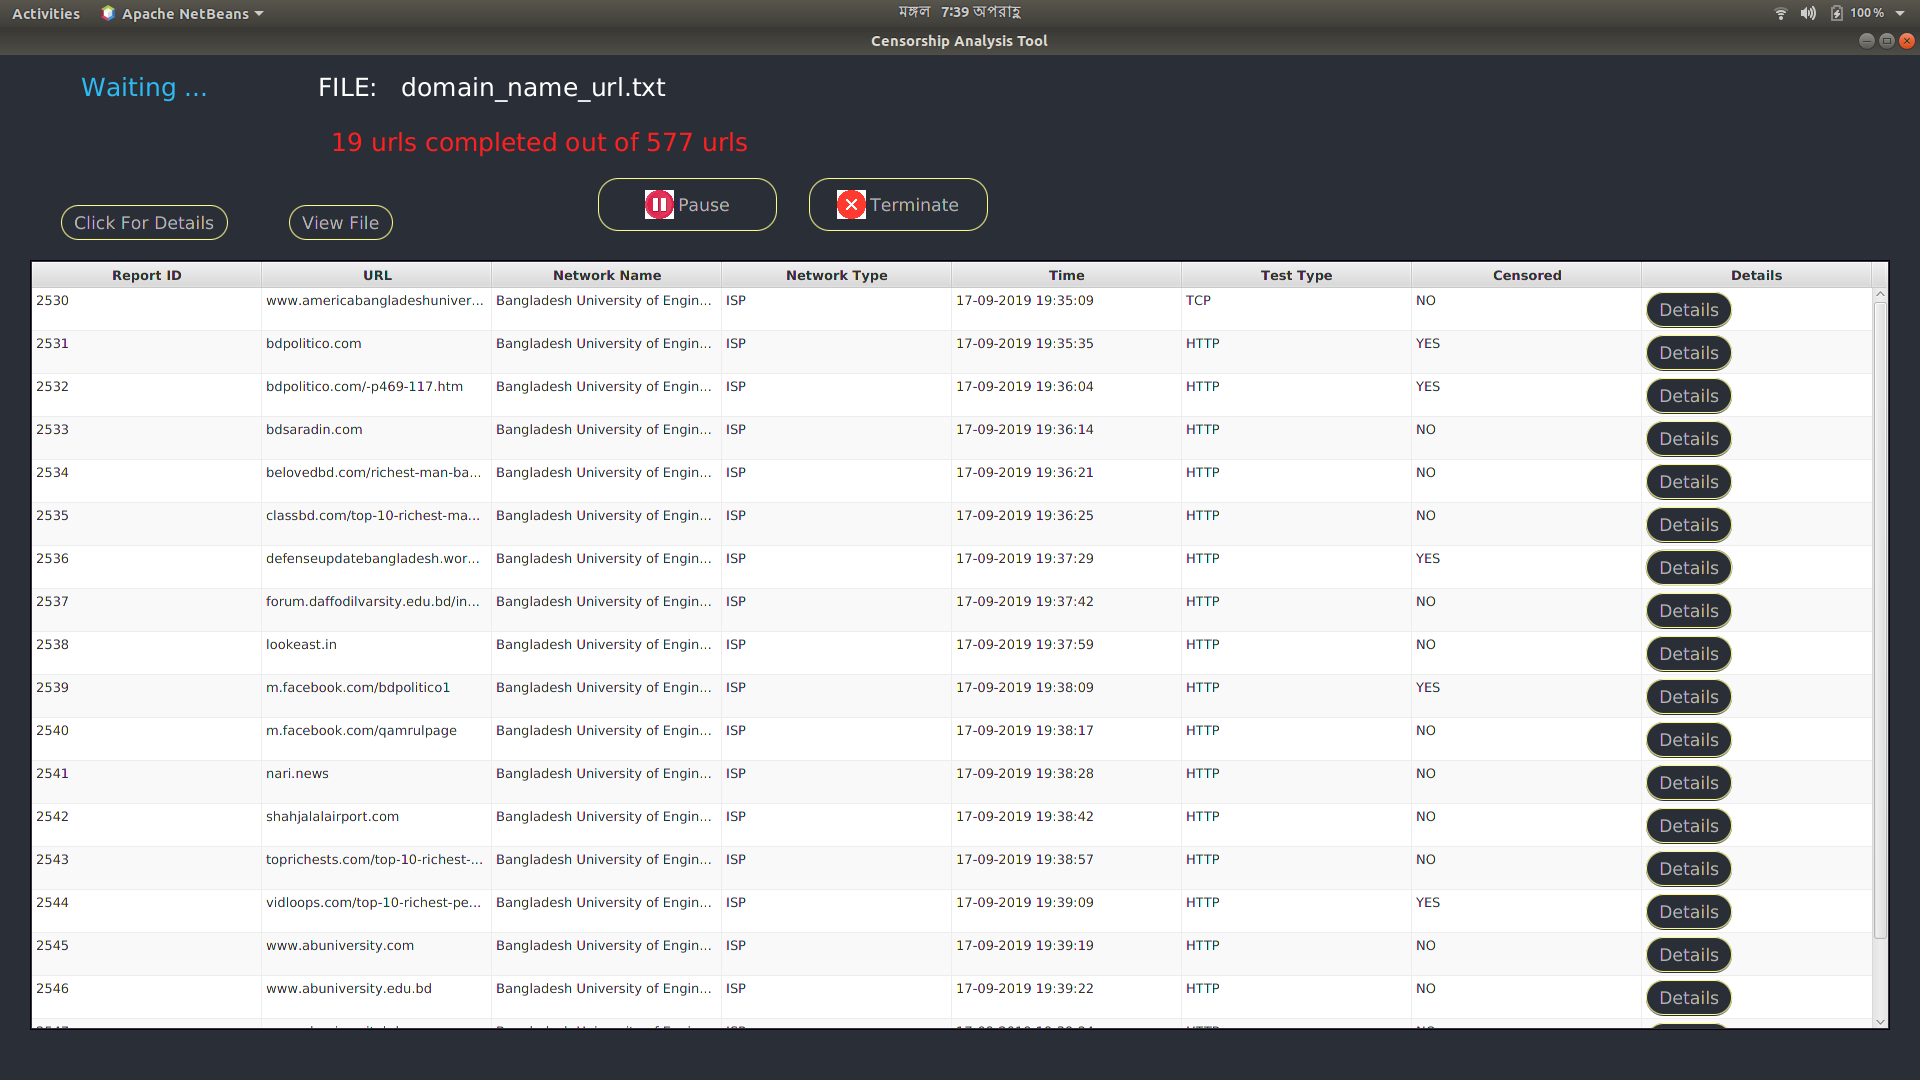
\includegraphics[width=\textwidth]{usersite/36completing.png}
    \caption{19 URLS completed out of 577}
    \label{fig:user36}
\end{figure}


\subsection{Fourth step: Checking statistics and downloading csv files}
If a user have enough input through desktop app, he can see his all history and statistics in graphical format. To see these information he should log in to the website. Here he should insert his username and password. If his credential is valid he will be redirected to his homepage. But if not error message will be shown. 
\begin{figure}[h]
    \centering
    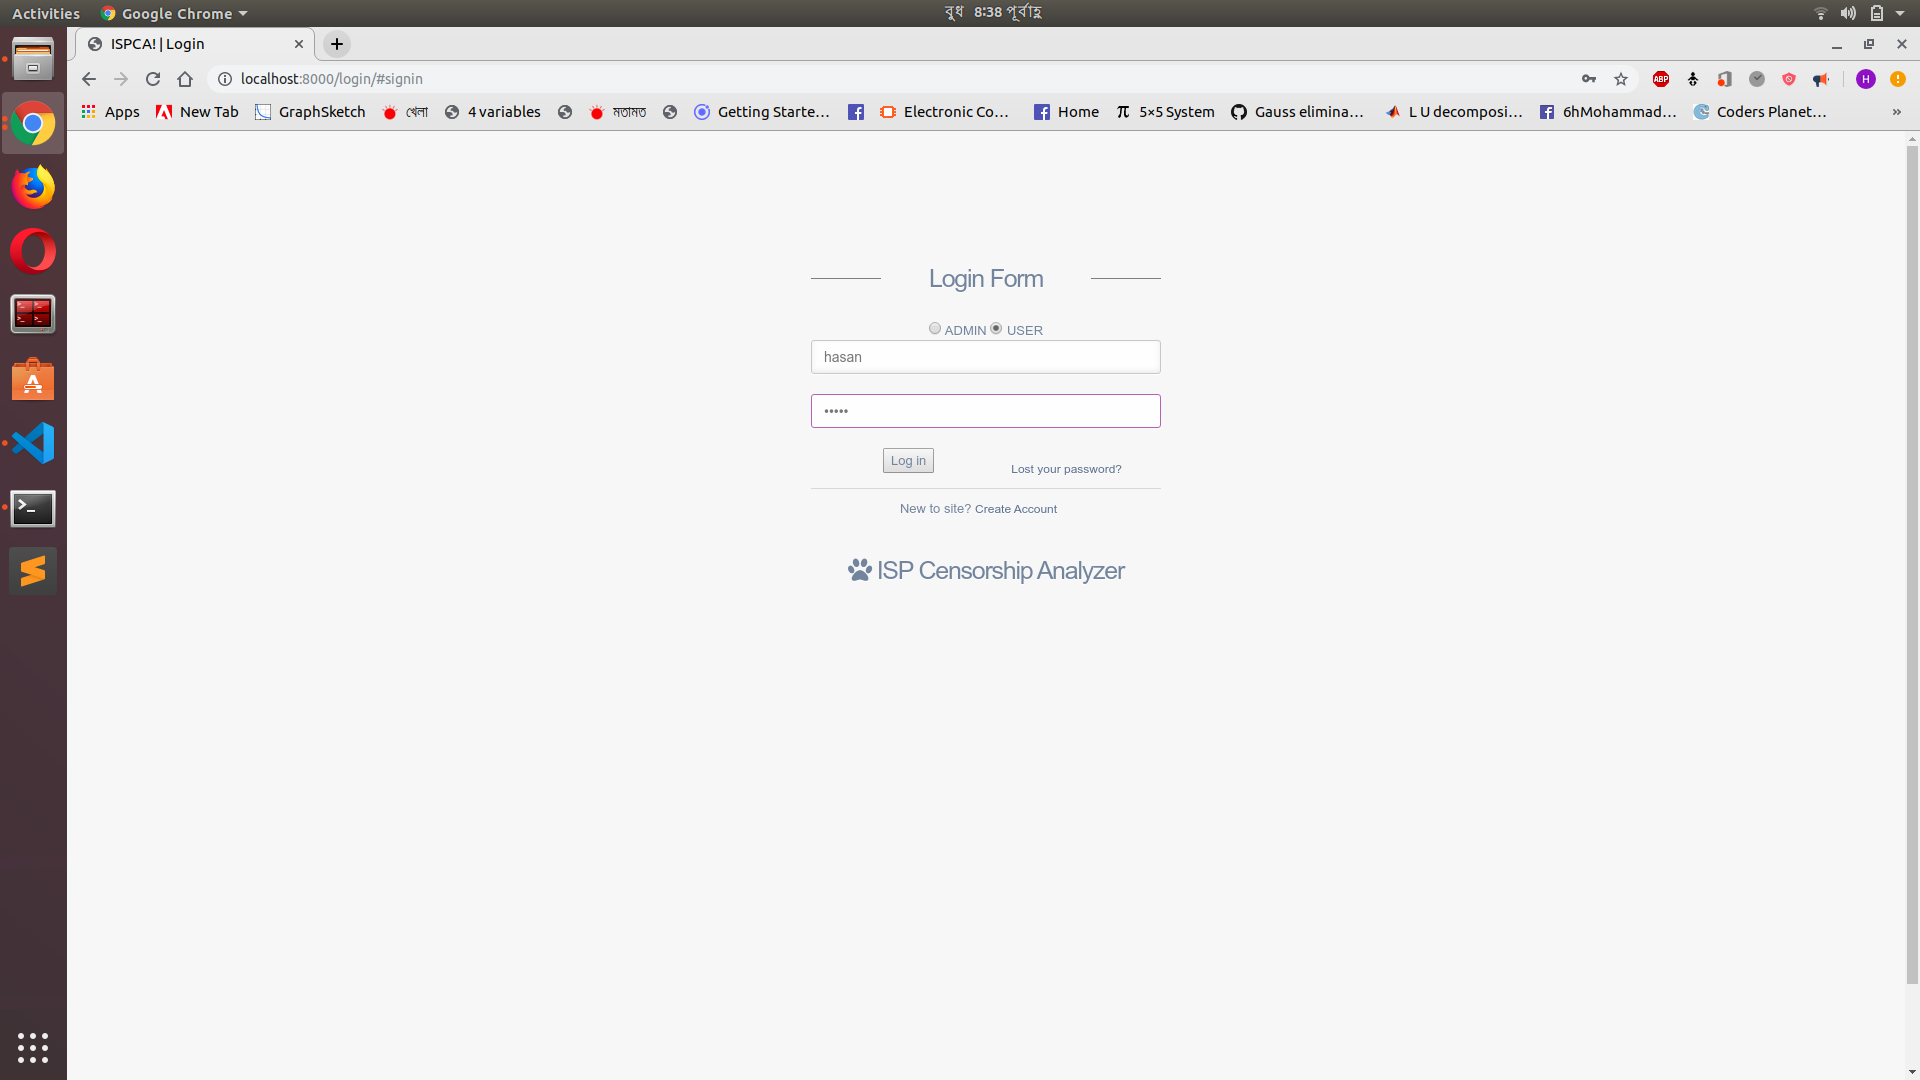
\includegraphics[width=\textwidth]{website/1login.png}
    \caption{Insert Compulsory field for login}
    \label{fig:web3}
\end{figure}

At homepage he will see all the sections and can navigate through the sections from side bar and can log out from the system. He can see total users of the system, his checked network, his total count tcp, dns, http censored website test. He will see the mostly checked ISP global IP and urls.

\begin{figure}[h]
    \centering
    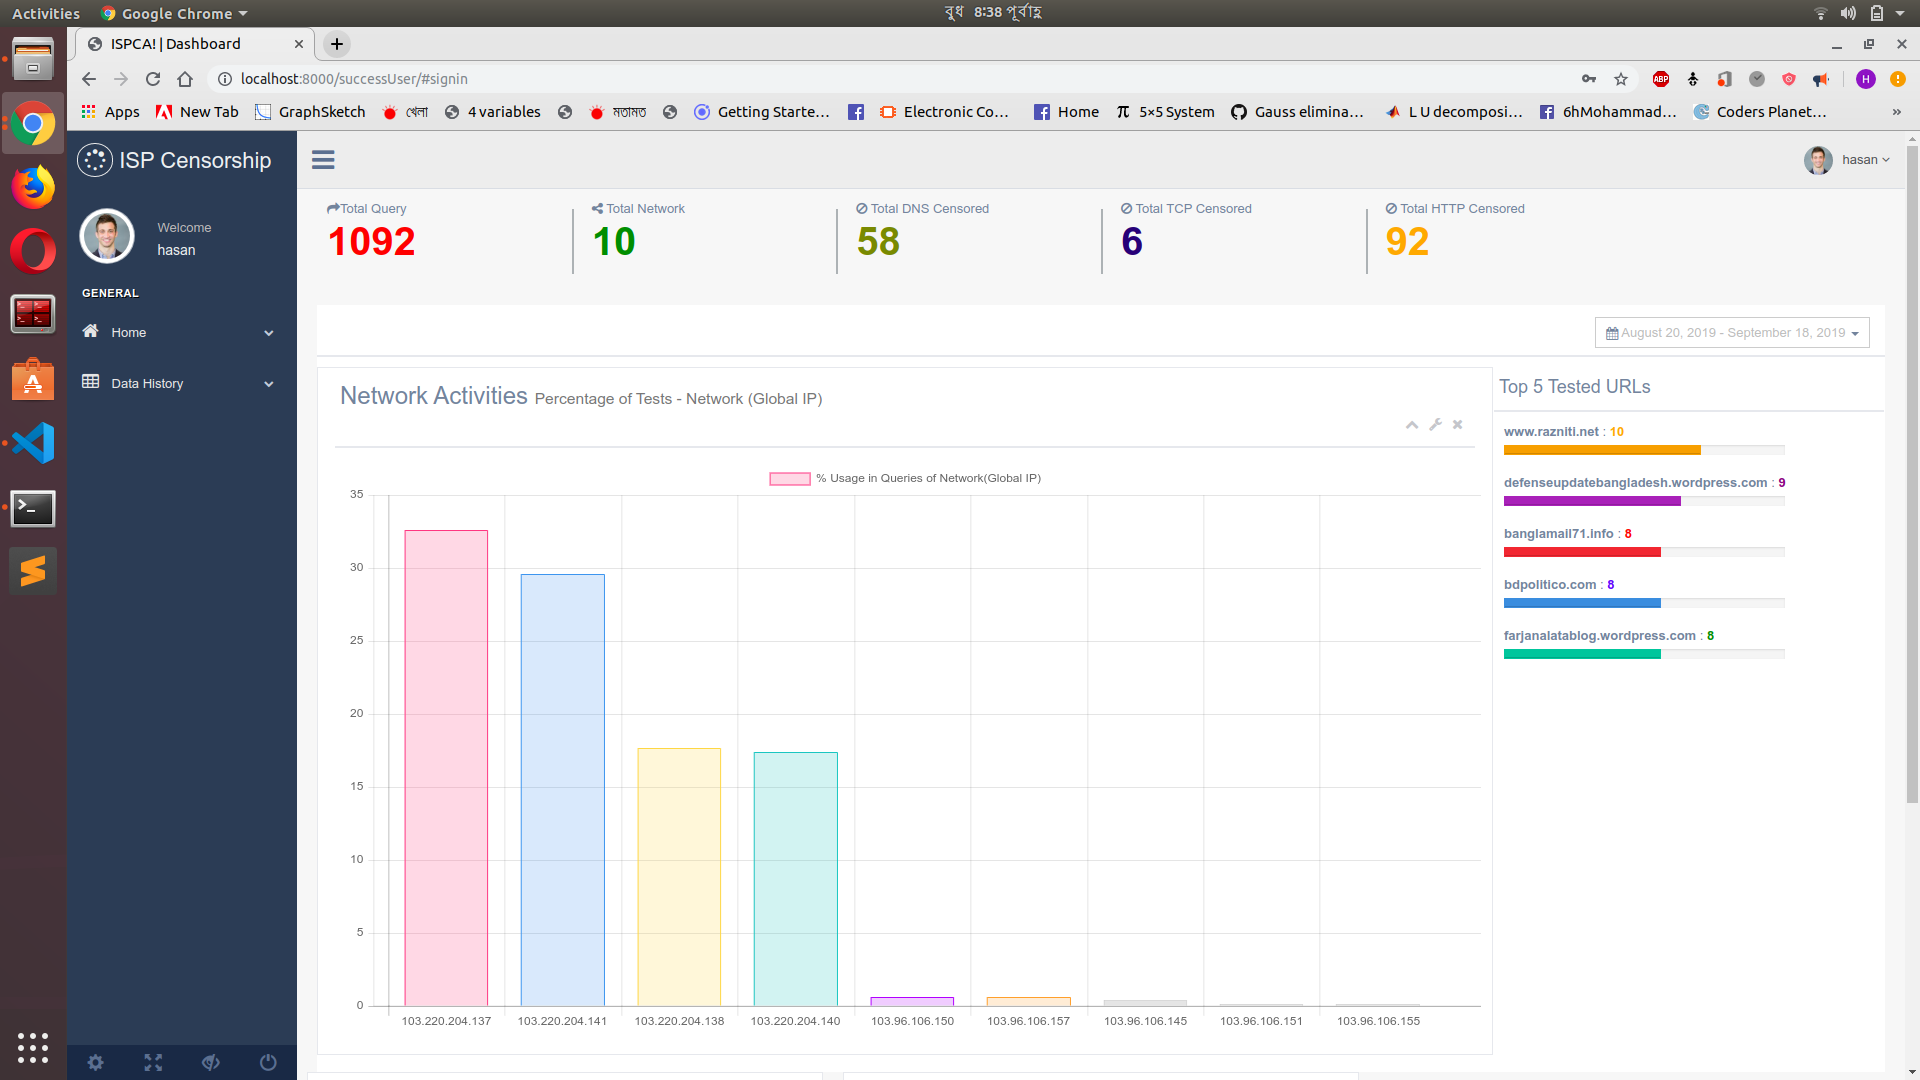
\includegraphics[width=\textwidth]{website/2userhome.png}
    \caption{Home page of user first part}
    \label{fig:web4}
\end{figure}
He can also see the percentage of censorship of his all visited url.

\begin{figure}[h]
    \centering
    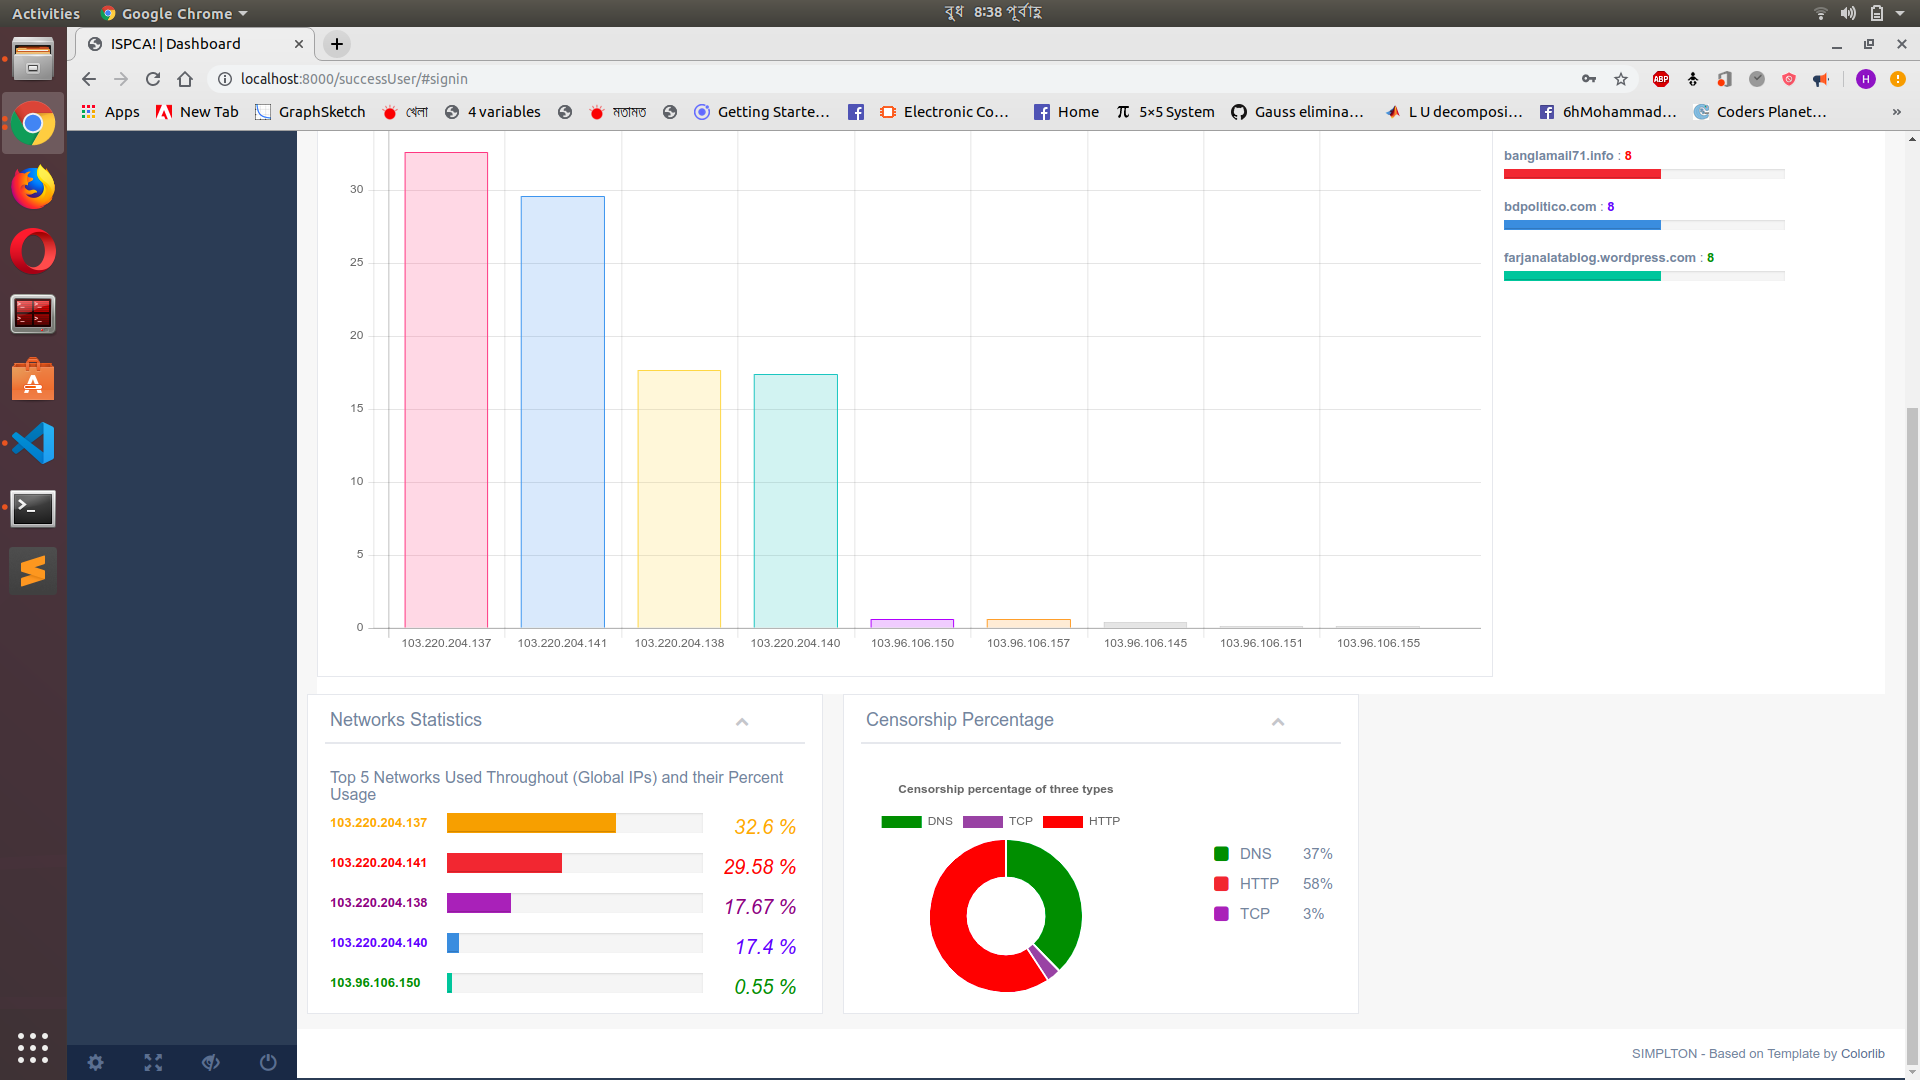
\includegraphics[width=\textwidth]{website/3userhome2.png}
    \caption{Insert Compulsory field for registration}
    \label{fig:web5}
\end{figure}

There are different kind of censorship analytics of a website. When a user go to \emph{Censorship Types} he can see the top 5 indicator of censorship of DNS, TCP and HTTP censorship in a pie chart.

\begin{figure}[h]
    \centering
    \includegraphics[width=\textwidth]{website/4cens.png}
    \caption{Showing top 5 all censorship type percentage of user}
    \label{fig:web6}
\end{figure}

\begin{figure}[h]
    \centering
    \includegraphics[width=\textwidth]{website/5dns.png}
    \caption{Showing top 5 DNS censorship type percentage of user}
    \label{fig:web7}
\end{figure}

\begin{figure}[h]
    \centering
    \includegraphics[width=\textwidth]{website/6tcp.png}
    \caption{Showing top 5 TCP censorship type percentage of user}
    \label{fig:web8}
\end{figure}



\begin{figure}[h]
    \centering
    \includegraphics[width=\textwidth]{website/7http.png}
    \caption{Showing top 5 HTTP censorship type percentage of user}
    \label{fig:web9}
\end{figure}

In \emph{Download CSV files} section a user can download his history in 4 file format DNS, TCP, HTTP and HTTPS format. He can analyze his data for further use. Here an example of DNS file is given below.

\begin{figure}[h]
    \centering
    \includegraphics[width=\textwidth]{website/8download.png}
    \caption{Downloading information as CSV file for all type censorship}
    \label{fig:web10}
\end{figure}

\begin{figure}[h]
    \centering
    \includegraphics[width=\textwidth]{website/8download2.png}
    \caption{Downloading information as CSV file for DNS type censorship}
    \label{fig:web11}
\end{figure}

\begin{figure}[h]
    \centering
    \includegraphics[width=\textwidth]{website/8download3.png}
    \caption{Downloaded DNS file as CSV format}
    \label{fig:web12}
\end{figure}

In \emph{Data} section a user can see all his data in tabular form. Here DNS, TCP, HTTP and HTTPS are given in photo format

\begin{figure}[h]
    \centering
    \includegraphics[width=\textwidth]{website/9dnsdetails.png}
    \caption{All data of DNS type censorship}
    \label{fig:web13}
\end{figure}

\begin{figure}[h]
    \centering
    \includegraphics[width=\textwidth]{website/10tcpdetails.png}
    \caption{All data of TCP type censorship}
    \label{fig:web14}
\end{figure}

\begin{figure}[h]
    \centering
    \includegraphics[width=\textwidth]{website/11httpdetails.png}
    \caption{All data of HTTP type censorship}
    \label{fig:web15}
\end{figure}

\begin{figure}[h]
    \centering
    \includegraphics[width=\textwidth]{website/12httpsdetails.png}
    \caption{All data of HTTPS type censorship}
    \label{fig:web16}
\end{figure}



\end{document}


